\documentclass[ngerman]{scrreprt}

\usepackage[utf8]{inputenc}
% T1 ist noetig, damit Woerter mit Umlauten und ss getrennt werden.
\usepackage[T1]{fontenc}
\usepackage{babel}
% hidelinks: ohne die Option zeichnet hyperref farbige Rahmen um jeden Verweis.
% Die sind Annotationen und werden mangels Print-Flag zwar nicht gedruckt, sind
% in jedem Betrachter aber sichtbar.
\usepackage[hidelinks]{hyperref}
\hypersetup{
  pdftitle={Analyse und Optimierung von MULTIFIT Algorithmen},
  pdfauthor={Fridjoff Hempel},
}

\usepackage[backend=biber,style=alphabetic]{biblatex}
\usepackage{csquotes}
% xurl bricht URLs an beliebiger Stelle -- ohne das laeuft der
% Williamson-Shmoys-Eintrag im Literaturverzeichnis 40,7 pt in den Rand.
\usepackage{xurl}

% Ein Titel mit langer, nicht umbrechbarer Formel (yue_kellerer_yu1988) erzwingt
% sonst ein Overfull \hbox; emergencystretch greift nur in genau solchen Zeilen.
\AtBeginBibliography{\emergencystretch=2em}
\usepackage{tikz}
\usepackage{graphicx}
\usepackage{float}
\usepackage{booktabs}
% Gleitobjekte duerfen keine \section-Grenze ueberschreiten; ohne diese Sperre
% wandern die Abbildungen und Tabellen aus Kapitel 5 in den jeweils folgenden
% Abschnitt. Kapitel 5 gliedert seine Versuchsreihen in Unterabschnitte, deshalb
% liegt dieselbe Sperre zusaetzlich vor jedem \subsection.
\usepackage[section]{placeins}
\let\ORGsubsection\subsection
\renewcommand{\subsection}{\FloatBarrier\ORGsubsection}
\usetikzlibrary{positioning,arrows.meta,fit}

% Mehr Gleitobjekte pro Seite zulassen, damit die Sperren oben keine
% halbleeren Seiten erzwingen.
\renewcommand{\topfraction}{0.9}
\renewcommand{\bottomfraction}{0.7}
\renewcommand{\textfraction}{0.1}
\renewcommand{\floatpagefraction}{0.75}
\setcounter{topnumber}{3}
\setcounter{bottomnumber}{2}
\setcounter{totalnumber}{4}

\usepackage{amsmath, amsfonts, amssymb, amsthm, cancel}
\usepackage{enumitem}

% Mit \def\OhneTodos{} von aussen (siehe unten) werden \todo und \listoftodos
% zu No-Ops -- fuer eine Abgabefassung ohne die offenen Punkte:
%   latexmk -jobname=main_ohne_todos -usepretex='\def\OhneTodos{}' main.tex
\ifdefined\OhneTodos
  \usepackage[disable]{todonotes}
\else
  \usepackage{todonotes}
\fi

\theoremstyle{definition}
\newtheorem{theorem}{Theorem}[chapter]
\newtheorem{lemma}[theorem]{Lemma}
\newtheorem{definition}[theorem]{Definition}
\newtheorem{korollar}[theorem]{Korollar}

\theoremstyle{remark}
\newtheoremstyle{myremark}%
  {\topsep}{\topsep}%
  {\normalfont}%
  {}%
  {\itshape}%
  {.}%
  {.5em}%
  {}%
\theoremstyle{myremark}
\newtheorem{bemerkung}[theorem]{Bemerkung}

\addbibresource{refs.bib}

% Kennzahlen der empirischen Auswertung; erzeugt von
% Implementation/Empirical_Tests/summary_tables.py
% Automatisch erzeugt von Implementation/Empirical_Tests/summary_tables.py
% Nicht von Hand bearbeiten.
\newcommand{\EvalInstanzen}{9\,092}
\newcommand{\EvalOptBekannt}{8\,512}
\newcommand{\EvalOhneOpt}{580}
\newcommand{\EvalLbBelegt}{580}
\newcommand{\EvalUnbestimmt}{0}
\newcommand{\EvalWins}{200}
\newcommand{\EvalTies}{8\,712}
\newcommand{\EvalLosses}{180}
\newcommand{\EvalWinsProzent}{2{,}2\,\%}
\newcommand{\EvalTiesProzent}{95{,}8\,\%}
\newcommand{\EvalLossesProzent}{2{,}0\,\%}
\newcommand{\EvalAbweichungen}{380}
\newcommand{\EvalRhoZwei}{3\,489}
\newcommand{\EvalRhoZweiProzent}{38{,}4\,\%}
\newcommand{\EvalRhoZweiAbw}{0}
\newcommand{\EvalRhoMaxAbw}{1{,}9475}
\newcommand{\EvalNMZwoelf}{760}
\newcommand{\EvalNMZwoelfAbw}{0}
\newcommand{\EvalNMMaxAbw}{10{,}0}
\newcommand{\EvalMaxRatioOpt}{1{,}1221}
\newcommand{\EvalMaxRatioOptFFD}{1{,}1221}
\newcommand{\EvalMaxRatioOptMFFD}{1{,}1221}
\newcommand{\EvalMaxRatioMffdFfd}{1{,}0495}
\newcommand{\EvalMinRatioMffdFfd}{0{,}9603}
\newcommand{\EvalOptimalFFD}{26{,}6\,\%}
\newcommand{\EvalZeitMedianMin}{1{,}037}
\newcommand{\EvalZeitMedianMax}{1{,}522}
\newcommand{\EvalSchranke}{1{,}1818}
\newcommand{\EvalRhoUnterZwei}{5\,603}
\newcommand{\EvalMaxRatioLb}{1{,}1368}
\newcommand{\EvalSteigungFFD}{1{,}14}
\newcommand{\EvalSteigungMFFD}{1{,}04}
\newcommand{\EvalKollapsMaxBereich}{$1{,}25 \le \rho < 1{,}5$}
\newcommand{\EvalKollapsMaxAnteil}{11{,}0\,\%}
\newcommand{\EvalKollapsLetzterAnteil}{0{,}9\,\%}
\newcommand{\EvalKNichtMonotonFFD}{0}
\newcommand{\EvalKNichtMonotonMFFD}{3}
\newcommand{\EvalKNichtMonotonMax}{4{,}9\,\%}
\newcommand{\EvalKNichtMonotonAlg}{MULTIFIT+MFFD}
\newcommand{\EvalKNichtMonotonInstanz}{p\_cmax-n10-m4-planted-U100-perturb0.05-seed1.txt}
\newcommand{\EvalKNichtMonotonVorher}{102}
\newcommand{\EvalKNichtMonotonNachher}{107}
\newcommand{\EvalKNichtMonotonKVorher}{5}
\newcommand{\EvalKNichtMonotonKNachher}{6}
\newcommand{\EvalKMax}{10}
\newcommand{\EvalKMittelEins}{1{,}2584}
\newcommand{\EvalKMaxEins}{1{,}4997}
\newcommand{\EvalKMittelZehn}{1{,}0154}
\newcommand{\EvalKMaxZehn}{1{,}1221}
\newcommand{\EvalKStabilMax}{5}
\newcommand{\EvalKStabilFuenf}{27{,}7\,\%}
\newcommand{\EvalKStabilNeun}{91{,}5\,\%}
\newcommand{\EvalKSchrankeStabil}{1{,}2131}
\newcommand{\EvalKSchrankeEins}{1{,}6818}
\newcommand{\EvalSchrankeK}{1{,}1828}
\newcommand{\EvalInstanzenFranca}{150}
\newcommand{\EvalOptBekanntFranca}{3}
\newcommand{\EvalRhoZweiFranca}{108}
\newcommand{\EvalRhoUnterZweiFranca}{42}
\newcommand{\EvalRhoZweiAnteilFranca}{72{,}0\,\%}
\newcommand{\EvalRhoMinFranca}{0{,}13}
\newcommand{\EvalRhoMaxFranca}{102{,}71}
\newcommand{\EvalNMMinFranca}{0{,}4}
\newcommand{\EvalNMMaxFranca}{200{,}0}
\newcommand{\EvalInstanzenFrangioni}{780}
\newcommand{\EvalOptBekanntFrangioni}{747}
\newcommand{\EvalRhoZweiFrangioni}{647}
\newcommand{\EvalRhoUnterZweiFrangioni}{133}
\newcommand{\EvalRhoZweiAnteilFrangioni}{82{,}9\,\%}
\newcommand{\EvalRhoMinFrangioni}{0{,}80}
\newcommand{\EvalRhoMaxFrangioni}{188{,}24}
\newcommand{\EvalNMMinFrangioni}{2{,}0}
\newcommand{\EvalNMMaxFrangioni}{200{,}0}
\newcommand{\EvalInstanzenLawrinenko}{3\,499}
\newcommand{\EvalOptBekanntLawrinenko}{3\,488}
\newcommand{\EvalRhoZweiLawrinenko}{289}
\newcommand{\EvalRhoUnterZweiLawrinenko}{3\,210}
\newcommand{\EvalRhoZweiAnteilLawrinenko}{8{,}3\,\%}
\newcommand{\EvalRhoMinLawrinenko}{0{,}70}
\newcommand{\EvalRhoMaxLawrinenko}{2{,}41}
\newcommand{\EvalNMMinLawrinenko}{2{,}0}
\newcommand{\EvalNMMaxLawrinenko}{3{,}0}
\newcommand{\EvalInstanzenBerndt}{3\,059}
\newcommand{\EvalOptBekanntBerndt}{3\,056}
\newcommand{\EvalRhoZweiBerndt}{2\,365}
\newcommand{\EvalRhoUnterZweiBerndt}{694}
\newcommand{\EvalRhoZweiAnteilBerndt}{77{,}3\,\%}
\newcommand{\EvalRhoMinBerndt}{0{,}80}
\newcommand{\EvalRhoMaxBerndt}{31{,}24}
\newcommand{\EvalNMMinBerndt}{2{,}0}
\newcommand{\EvalNMMaxBerndt}{50{,}0}
\newcommand{\EvalInstanzenPlanted}{1\,604}
\newcommand{\EvalOptBekanntPlanted}{1\,218}
\newcommand{\EvalRhoZweiPlanted}{80}
\newcommand{\EvalRhoUnterZweiPlanted}{1\,524}
\newcommand{\EvalRhoZweiAnteilPlanted}{5{,}0\,\%}
\newcommand{\EvalRhoMinPlanted}{1{,}00}
\newcommand{\EvalRhoMaxPlanted}{4{,}11}
\newcommand{\EvalNMMinPlanted}{2{,}0}
\newcommand{\EvalNMMaxPlanted}{10{,}0}
\newcommand{\EvalRhoMedianFrangioniBimodal}{18{,}7}
\newcommand{\EvalRhoZweiAnteilFrangioniBimodal}{84{,}6\,\%}
\newcommand{\EvalRhoMedianFrangioniGleich}{9{,}7}
\newcommand{\EvalRhoZweiAnteilFrangioniGleich}{81{,}3\,\%}
\newcommand{\EvalPlantedGeneriert}{540}
\newcommand{\EvalPlantedOriginale}{1\,064}
\newcommand{\EvalPlantedOriginaleOpt}{1\,038}
\newcommand{\EvalPlantedRNull}{461}
\newcommand{\EvalPlantedRPositiv}{757}

% automatisch erzeugt von Empirical_Tests/summary_tables_hm.py
% nicht von Hand bearbeiten
\newcommand{\HmInstanzen}{1\,080}
\newcommand{\HmInstanzenSzenario}{360}
\newcommand{\HmArme}{5}
\newcommand{\HmOptBekannt}{1\,080}
\newcommand{\HmOhneOpt}{0}
\newcommand{\HmDegeneriert}{24}
\newcommand{\HmDAbweichung}{2}
\newcommand{\HmDMin}{3}
\newcommand{\HmDMax}{6}
\newcommand{\HmNMin}{15}
\newcommand{\HmNMax}{160}
\newcommand{\HmMMin}{5}
\newcommand{\HmMMax}{20}
\newcommand{\HmRhoMin}{0{,}52}
\newcommand{\HmRhoMax}{7{,}74}
\newcommand{\HmSchranke}{1{,}1818}
\newcommand{\HmSchrankeK}{1{,}1828}
\newcommand{\HmDMinusEins}{5}
\newcommand{\HmMaxRatioOptffd}{1{,}1429}
\newcommand{\HmOptimalffd}{56{,}3\,\%}
\newcommand{\HmZeitMedianffd}{0{,}6}
\newcommand{\HmMaxRatioOptjansen}{1{,}0317}
\newcommand{\HmOptimaljansen}{97{,}3\,\%}
\newcommand{\HmZeitMedianjansen}{125{,}4}
\newcommand{\HmWinsjansen}{453}
\newcommand{\HmTiesjansen}{619}
\newcommand{\HmLossesjansen}{8}
\newcommand{\HmMaxRatioOptjansendual}{1{,}0303}
\newcommand{\HmOptimaljansendual}{98{,}6\,\%}
\newcommand{\HmZeitMedianjansendual}{25{,}7}
\newcommand{\HmWinsjansendual}{457}
\newcommand{\HmTiesjansendual}{618}
\newcommand{\HmLossesjansendual}{5}
\newcommand{\HmMaxRatioOptgglp}{1{,}0317}
\newcommand{\HmOptimalgglp}{92{,}4\,\%}
\newcommand{\HmZeitMediangglp}{12{,}8}
\newcommand{\HmWinsgglp}{446}
\newcommand{\HmTiesgglp}{633}
\newcommand{\HmLossesgglp}{1}
\newcommand{\HmMaxRatioOptggip}{1{,}0000}
\newcommand{\HmOptimalggip}{100{,}0\,\%}
\newcommand{\HmZeitMedianggip}{19{,}4}
\newcommand{\HmWinsggip}{461}
\newcommand{\HmTiesggip}{619}
\newcommand{\HmLossesggip}{0}
\newcommand{\HmMaxRatioOptReferenz}{1{,}0000}
\newcommand{\HmZuUnrechtFfd}{774}
\newcommand{\HmZuUnrechtJansen}{38}
\newcommand{\HmZuUnrechtJansendual}{0}
\newcommand{\HmZuUnrechtGglp}{95}
\newcommand{\HmZuUnrechtGgip}{0}
\newcommand{\HmJansenNichtMonotonSpur}{0}
\newcommand{\HmNichtMonotonInstanz}{\texttt{HM\_dense\_d5\_n0080\_m10\_7}}
\newcommand{\HmNichtMonotonC}{327}
\newcommand{\HmNichtMonotonCPlus}{328}
\newcommand{\HmNichtMonotonJ}{10}
\newcommand{\HmNichtMonotonJPlus}{11}
\newcommand{\HmFMax}{6}
\newcommand{\HmFMedian}{3}
\newcommand{\HmFGleichD}{32{,}4\,\%}
\newcommand{\HmRestAufrufe}{6\,497}
\newcommand{\HmRestBinsMedian}{2}
\newcommand{\HmRestBinsMax}{5}
\newcommand{\HmRestUnterF}{5\,292}
\newcommand{\HmRestUnterFAnteil}{81{,}5\,\%}
\newcommand{\HmRestQuelleFfd}{4\,164}
\newcommand{\HmRestQuelleMuster}{2\,333}
\newcommand{\HmRestQuelleOhne}{627}
\newcommand{\HmEpsGleicheAkzeptanz}{1\,080}
\newcommand{\HmEpsAkzeptanzInstanzen}{1\,080}
\newcommand{\HmEpsSchlechterRef}{15}
\newcommand{\HmEpsUeberlastMax}{1{,}0303}
\newcommand{\HmJansenFehlablehnungInstanzen}{29}
\newcommand{\HmJansenVerlusteMitFehlablehnung}{8}
\newcommand{\HmJansenVerlusteOhne}{0}
\newcommand{\HmJansenSchlechterFFD}{8}
\newcommand{\HmJansenBesserFFD}{453}
\newcommand{\HmGGAufrufe}{7\,124}
\newcommand{\HmGGZertifiziert}{1\,485}
\newcommand{\HmGGUnentschieden}{95}
\newcommand{\HmGGUnentschiedenAnteil}{1{,}33\,\%}
\newcommand{\HmGGRundungsverlustMax}{1}
\newcommand{\HmGGOhneVerlust}{98{,}5\,\%}
\newcommand{\HmQMax}{1\,378\,772}
\newcommand{\HmQMedian}{312}
\newcommand{\HmGGGleichOpt}{6\,945}
\newcommand{\HmGGPlusEins}{95}
\newcommand{\HmGGMaxUeberOpt}{1}
\newcommand{\HmGGVergleiche}{7\,040}
\newcommand{\HmJansenVergleiche}{7\,092}
\newcommand{\HmJansenGleichOpt}{7\,049}
\newcommand{\HmJansenPlusEins}{43}
\newcommand{\HmJansenUeberOpt}{0{,}6\,\%}
\newcommand{\HmJansenMaxUeberOpt}{1}
\newcommand{\HmJansenMilpMax}{8}
\newcommand{\HmJansenMilpMedian}{6}
\newcommand{\HmJansenMilpSchranke}{8}
\newcommand{\HmMsProMilpJansen}{3{,}18}
\newcommand{\HmMsProModellGgip}{2{,}92}
\newcommand{\HmEpsMax}{0{,}0370}
\newcommand{\HmEpsTheorieMin}{0{,}0909}
\newcommand{\HmEpsTheorieMax}{0{,}2000}
\newcommand{\HmLastFaktorMax}{1{,}0370}
\newcommand{\HmEpsPositiv}{30}
\newcommand{\HmEpsAufrufe}{5\,595}
\newcommand{\HmGgRZweiAnteil}{75{,}0\,\%}
\newcommand{\HmGgRZweiInstanzen}{810}
\newcommand{\HmDegOptPMax}{23}
\newcommand{\HmDegAlleOptimal}{alle}
\newcommand{\HmDegRhoMax}{0{,}99}
\newcommand{\HmDBenchMedianMin}{20}
\newcommand{\HmDBenchMedianMax}{81}
\newcommand{\HmDBenchMax}{2\,363}
\newcommand{\HmSkalBudget}{200\,000}
\newcommand{\HmSkalZuege}{2\,000}
\newcommand{\HmSkalDMaxAlle}{4}
\newcommand{\HmSkalDLuecke}{5}
\newcommand{\HmSkalSzenarioLuecke}{Asymmetric}
\newcommand{\HmSkalInstanzen}{120}
\newcommand{\HmSkalNMin}{40}
\newcommand{\HmSkalNMax}{40\,000}
\newcommand{\HmSkalMMax}{5\,000}
\newcommand{\HmSkalRatio}{8}
\newcommand{\HmSkalNFaktor}{1\,000}
\newcommand{\HmSkalSchnittpunkt}{1\,400}
\newcommand{\HmSkalFaktorffd}{2\,118{,}2}
\newcommand{\HmSkalZeitMaxffd}{979{,}8}
\newcommand{\HmSkalFaktorjansen}{9{,}4}
\newcommand{\HmSkalZeitMaxjansen}{991{,}1}
\newcommand{\HmSkalFaktorjansendual}{6{,}3}
\newcommand{\HmSkalZeitMaxjansendual}{142{,}2}
\newcommand{\HmSkalFaktorgglp}{8{,}5}
\newcommand{\HmSkalZeitMaxgglp}{105{,}4}
\newcommand{\HmSkalFaktorggip}{6{,}8}
\newcommand{\HmSkalZeitMaxggip}{124{,}3}
\newcommand{\HmSkalFaktorMin}{6{,}3}
\newcommand{\HmSkalFaktorMax}{9{,}4}


\title{Analyse und Optimierung von MULTIFIT Algorithmen}
\author{Fridjoff Hempel}
\date{\today}

\begin{document}

\maketitle
\chapter*{Zusammenfassung}

Diese Arbeit untersucht MULTIFIT, ein Approximationsverfahren von Coffman, Garey und Johnson
(1978) für die Makespan-Minimierung auf identischen Maschinen.
Das Verfahren rät eine Schranke an den Makespan und überlässt dem Bin-Packing-Verfahren First
Fit Decreasing (FFD) als Subroutine die Frage, ob die Aufgaben in ebenso viele Behälter dieser
Größe passen, wie Maschinen vorhanden sind; eine Binärsuche verengt die Schranke anschließend.
Im ersten Teil der Arbeit wird die Performanzanalyse von MULTIFIT geschlossen aufbereitet: Die
auf Coffman, Garey und Johnson (1978) zurückgehende Schranke $5/4$ für das Grenzverhältnis, an
welchem das im schlechtesten Fall erreichte Verhältnis von erzeugtem zu optimalem Makespan
hängt, wird vollständig bewiesen und mit dem Makespan nach $k$ Suchschritten verbunden; die
schärfere Schranke $13/11$ von Cao (1995) wird eingeordnet, und an einer Instanz von Friesen
(1984) wird gezeigt, dass sie sich für mindestens $13$ Maschinen nicht verbessern lässt.
Im zweiten Teil der Arbeit wird die Subroutine von MULTIFIT ausgetauscht.
Für Modified First Fit Decreasing (MFFD) von Johnson und Garey (1985) als Subroutine wird
gezeigt, dass es innerhalb von MULTIFIT dieselbe Zuordnung wie FFD liefert, sobald die mittlere
Maschinenlast mindestens doppelt so groß ist wie die größte Aufgabe.
Der $\mathrm{OPT}+1$-Algorithmus von Jansen und Solis-Oba (2010) für Instanzen mit $d$
verschiedenen Aufgabengrößen wird zu einem $\varepsilon$-dualen Verfahren im Sinne von Hochbaum
und Shmoys (1987) umgebaut, welches höchstens die optimale Binzahl verwendet und dafür die
Kapazität um den Faktor $1+\varepsilon$ überschreiten darf; MULTIFIT erreicht damit einen
Makespan von höchstens $(1+\varepsilon)(1+2^{-k})$ mal dem Optimum, wobei
$\varepsilon = 1/(2d-1)$ ist.
Für das Konfigurations-LP von Gilmore und Gomory (1961) trägt die beim Runden entstehende
Schranke dieselbe Schlussweise dagegen nicht.
Sämtliche untersuchten Verfahren sind implementiert und praktisch getestet worden.
Auf \EvalInstanzen{} Benchmark-Instanzen überschreitet kein gemessenes Verhältnis zum optimalen
Makespan den Wert $13/11$, und MFFD liefert keinen systematisch kleineren Makespan als FFD.
Auf \HmInstanzen{} Instanzen mit wenigen verschiedenen Aufgabengrößen liefert MULTIFIT mit dem
$\mathrm{OPT}+1$-Algorithmus auf \HmJansenBesserFFD{} Instanzen einen kleineren, auf
\HmJansenSchlechterFFD{} jedoch einen größeren Makespan als mit FFD.
Eine bessere Bin-Packing-Garantie sichert somit keinen kleineren Makespan; dafür kommt es darauf
an, bei welchen der getesteten Schranken die Subroutine die Maschinenzahl unterschreitet und, wo
sie die Schranke überschreiten darf, wie weit sie das tut.

\tableofcontents
\listoftodos

\chapter{Einleitung}
\label{chap:einleitung}

Ein Betrieb verteilt eingehende Aufträge auf mehrere gleich schnelle Maschinen, ein Rechenzentrum
verteilt Rechenaufträge auf die Knoten eines Clusters.
In beiden Fällen ist dieselbe Frage zu beantworten: Welche Aufgabe gehört auf welche Maschine?
Entscheidend ist dabei nicht die Summe der Bearbeitungszeiten, sondern der Zeitpunkt, zu dem die
zuletzt beschäftigte Maschine ihre Arbeit beendet.
Dieser Zeitpunkt heißt \emph{Makespan}, und seine Minimierung ist der Gegenstand dieser Arbeit.

Formal sind $n$ Aufgaben mit bekannten Bearbeitungszeiten und $m$ identische Maschinen gegeben.
Jede Aufgabe läuft ohne Unterbrechung auf genau einer Maschine; gesucht ist eine Zuordnung mit
kleinstmöglichem Makespan.
In der Notation von \textcite{graham1979} trägt dieses Problem den Namen $P\,\|\,C_{\max}$.
Kapitel~\ref{chap:grundlagen} führt diese Notation zusammen mit den übrigen Bezeichnungen ein.
Das zugehörige Entscheidungsproblem ist NP-vollständig \cite{garey_johnson1979}; sofern
$\mathrm{P} \ne \mathrm{NP}$ gilt, berechnet folglich kein Algorithmus mit polynomieller Laufzeit
den minimalen Makespan.
Gefragt sind deshalb Verfahren, welche schnell eine Zuordnung liefern und deren
\emph{Approximationsgüte} sich beweisen lässt.
Diese Güte ist der Faktor, um den der erzeugte Makespan den optimalen im schlechtesten Fall
höchstens übersteigt.

\paragraph{Bekannte Ansätze.}
Der erste Algorithmus mit einer solchen Garantie stammt von \textcite{graham1966}; mit dem
Makespan-Problem nimmt die Analyse beweisbar guter Verfahren ihren Ausgang
\cite[S.~145]{hochbaum_shmoys_1987}.
Sein List-Scheduling durchläuft die Aufgaben in einer gegebenen Reihenfolge und legt jede auf
die gerade am wenigsten belastete Maschine; der erzeugte Makespan übersteigt das Optimum dabei um
höchstens den Faktor $2 - 1/m$.
Dieser Faktor ist \emph{scharf}, das heißt, kleiner lässt er sich nicht wählen: Es gibt
Instanzen, auf welchen ihm das Verhältnis von erzeugtem zu optimalem Makespan beliebig nahe
kommt \cite[S.~1571]{graham1966}.
Werden die Aufgaben zuvor absteigend sortiert, so sinkt der Faktor auf $4/3 - 1/(3m)$, und auch
dieser Wert ist scharf \cite[Theorem~2]{graham1969}.
Diese Regel ist unter dem Namen \emph{Longest Processing Time} bekannt.

Einen anderen Weg gehen \textcite{coffman1978} mit MULTIFIT.
Statt die Aufgaben unmittelbar zu verteilen, rät das Verfahren eine Schranke $C$ an den Makespan
und überlässt einem Bin-Packing-Algorithmus die Frage, ob die Aufgaben in $m$ Behälter der
Kapazität $C$ passen.
Beides ist dieselbe Frage, denn eine solche Packung ist genau eine Zuordnung, bei der keine
Maschine länger als $C$ arbeitet.
Dieser Algorithmus heißt im Folgenden \emph{Subroutine}; \textcite{coffman1978} setzen dafür
First Fit Decreasing (FFD) ein, welches die Aufgaben absteigend sortiert und jede in den ersten
Behälter legt, in den sie noch passt.
Die Packung erzeugt damit die Subroutine; eine Binärsuche über $C$, nach $k$
Halbierungsschritten abgebrochen, wählt unter den akzeptierten Schranken die kleinste aus und
gibt deren Packung zurück.
Die Güte von MULTIFIT hängt damit an einer rein kombinatorischen Größe, dem
\emph{Grenzverhältnis} $r_m$: Übersteigt eine Kapazität den optimalen Makespan um mehr als den
Faktor $r_m$, so kommt FFD mit $m$ Behältern aus (Definition~\ref{def:rm}).
Für diesen Wert weisen \textcite{coffman1978} zunächst $r_m \le 1{,}22$ nach.
Über \textcite{friesen1984} und \textcite{yue1990} ist die Schranke später auf $13/11$ verschärft
worden, und \textcite{cao1995} gibt dafür einen vollständigen Beweis;
Abschnitt~\ref{sec:chronologie} stellt diese Entwicklung im Einzelnen dar.

Beliebig nah an das Optimum führen Approximationsschemata: Zu jeder vorgegebenen Genauigkeit
$\varepsilon > 0$ liefern sie eine Zuordnung mit einem Makespan von höchstens $(1+\varepsilon)$
mal dem Optimum.
Für eine feste Maschinenzahl gibt \textcite{sahni1976} ein solches Schema an, und
\textcite{hochbaum_shmoys_1987} behandeln den Fall beliebiger Maschinenzahl über \emph{duale}
Approximation, bei der nicht die Zahl der Behälter, sondern deren Kapazität überschritten werden
darf.
Bezahlt wird die Genauigkeit mit Laufzeit: Das Schema von Hochbaum und Shmoys läuft in
$O\bigl((n/\varepsilon)^{1/\varepsilon^{2}}\bigr)$, was die Autoren selbst als nicht praktikabel
bezeichnen \cite[S.~146]{hochbaum_shmoys_1987}.
MULTIFIT liegt zwischen beiden Linien, denn seine Güte ist fest, jeder Suchschritt kostet aber
nur einen einzigen Aufruf der Subroutine.
Einmaliges Sortieren und $k+1$ solche Aufrufe ergeben eine Laufzeit in $O(k\,n \log n)$, bei
fester Suchtiefe also $O(n \log n)$ (Abschnitt~\ref{sec:multifit}).

Verbessert worden ist MULTIFIT auch, ohne die Subroutine anzutasten.
\textcite{friesen_langston1986} ersetzen den Zweig, welcher eine Kapazität verwirft, durch eine
Reparatur: Eine beschränkte Zahl besonders ungünstig belegter Maschinen wird zusammen mit den
dabei übrig gebliebenen Aufgaben optimal neu belegt.
Das Verhältnis von erzeugtem zu optimalem Makespan sinkt dadurch auf $72/61$ und liegt damit
unter $13/11$; asymptotisch ist dieser Wert scharf, und die Laufzeitordnung $O(n \log n)$
bleibt erhalten.
Diese Arbeit geht den anderen Weg und lässt die Suche unangetastet.

Welche Subroutine dort steht, ist ein eigener Strang der Literatur.
FFD benötigt höchstens $11/9$ mal so viele Behälter wie eine optimale Packung, zuzüglich einer
additiven Konstanten; diese Schranke ist scharf \cite{dosa2007}.
Für Modified First Fit Decreasing (MFFD) ist mit $71/60$ eine kleinere obere Schranke bewiesen
\cite{johnson_garey1985, yue_zhang1995}.
Da $11/9$ scharf ist, fällt das asymptotische Worst-Case-Verhältnis von MFFD damit echt kleiner
aus als jenes von FFD; ob MFFD den Wert $71/60$ überhaupt annimmt, ist dagegen offen.
Kommen in einer Instanz nur wenige verschiedene Aufgabengrößen vor, so erreicht der
$\mathrm{OPT}+1$-Algorithmus von \textcite{jansen_solisoba2010} sogar eine Packung mit höchstens
einem Behälter über dem Optimum; sein Name benennt genau diese Garantie.
Ob ein solcher Vorteil den Makespan von MULTIFIT verkleinert, ist damit allerdings nicht gesagt:
Dessen Gütegarantie beruht auf einer bestimmten Eigenschaft von FFD, welche eine schärfere
Bin-Packing-Schranke nicht ersetzt.

Daneben stehen exakte Verfahren, etwa die Arc-Flow-Modelle von \textcite{mrad2018} oder die
Suchverfahren von \textcite{akram2025}.
Sie liefern den minimalen Makespan, besitzen im schlechtesten Fall aber keine polynomielle
Laufzeit; in Kapitel~\ref{chap:evaluation} dienen ihre publizierten Werte als Vergleichsgrundlage.

\paragraph{Beitrag dieser Arbeit.}
Die Arbeit verfolgt zwei Ziele.
Das erste ist eine geschlossene Aufbereitung der Performanzanalyse von MULTIFIT.
\textcite{cao1995} dient dabei als primäre Quelle, setzt die Ergebnisse von
\textcite{coffman1978} jedoch über weite Strecken voraus und führt einzelne Beweisschritte nur
knapp aus.
Kapitel~\ref{chap:performanz} führt deshalb die Herleitung der Schranke $r_m \le 5/4$
vollständig aus und verbindet sie in Theorem~\ref{thm:guete} mit dem Makespan, den MULTIFIT nach
$k$ Suchschritten zurückgibt.
Die schärfere Schranke $13/11$ wird eingeordnet und ihre Beweisidee dargestellt, nicht aber
bewiesen; Caos Fallunterscheidung bleibt außerhalb des Umfangs dieser Arbeit.
Die zugehörige untere Schranke wird dagegen geführt, denn eine Instanz von \textcite{friesen1984}
belegt $r_m \ge 13/11$ für alle $m \ge 13$.

Das zweite Ziel betrifft die Subroutine, denn innerhalb von MULTIFIT ist sie austauschbar.
Kapitel~\ref{kap:alternative} untersucht drei Alternativen theoretisch.
Zwei Ergebnisse daraus sind eigenständige Beiträge.
Zum einen gibt das Kollaps-Lemma eine Klasse von Instanzen an, auf der MFFD und FFD innerhalb von
MULTIFIT stets dieselbe Zuordnung erzeugen.
Zum anderen wird der $\mathrm{OPT}+1$-Algorithmus von \textcite{jansen_solisoba2010} zu einem
$\varepsilon$-dualen Approximationsalgorithmus umgebaut.
Zusammen mit dem Ergebnis von \textcite{hochbaum_shmoys_1987} garantiert dieser Umbau nach $k$
Suchschritten einen Makespan von höchstens $(1+\varepsilon)(1+2^{-k})$ mal dem Optimum.
Als dritte Alternative dient das Konfigurations-LP von \textcite{gilmore_gomory1961}, welches
jede mögliche Füllung eines Behälters als eigene Variable führt und die Ganzzahligkeit zunächst
fallen lässt.
Für dieses Programm wird umgekehrt gezeigt, dass die beim Runden entstehende Schranke gerade
nicht ausreicht, um die Gütegarantie von MULTIFIT zu tragen.

Was der Austausch praktisch bewirkt, misst Kapitel~\ref{chap:evaluation} in zwei Versuchsreihen.
Die erste vergleicht FFD und MFFD auf \EvalInstanzen{} Instanzen aus fünf publizierten
Benchmark-Datensätzen, die zweite vier Subroutinen für Instanzen mit wenigen verschiedenen
Aufgabengrößen auf \HmInstanzen{} eigens erzeugten Instanzen.
Kein gemessenes Verhältnis überschreitet dabei $13/11$ - für MULTIFIT+FFD liegt dieser Wert
knapp unter der bewiesenen Schranke $13/11 + 2^{-k}$, für die übrigen Kombinationen ist er
lediglich eine Vergleichslinie.
Zugleich zeigen beide Reihen, dass aus einer schärferen Bin-Packing-Garantie kein kleinerer
Makespan folgt.

\paragraph{Aufbau.}
Kapitel~\ref{chap:grundlagen} legt die Grundlagen: Problemstellung und Notation, Bin Packing mit
FFD sowie der Algorithmus MULTIFIT samt seinem Startintervall.
Kapitel~\ref{chap:performanz} enthält die Performanzanalyse, Kapitel~\ref{kap:alternative} die
drei alternativen Subroutinen und Kapitel~\ref{chap:evaluation} die empirische Auswertung.
Kapitel~\ref{chap:fazit} fasst die Ergebnisse zusammen und benennt die offen gebliebenen Fragen.
Sämtliche Implementierungen und Messskripte liegen unter
\url{https://github.com/hempllll/MultiFit-BscThs}; den Versuchsaufbau beschreibt
Abschnitt~\ref{sec:versuchsaufbau}.

\chapter{Grundlagen}
\label{chap:grundlagen}

\section{Scheduling auf identischen Maschinen}
\label{sec:problem}

\begin{definition}[Instanz und Makespan]
\label{def:instanz}
Eine \emph{Instanz} $\Gamma$ besteht aus $n$ Aufgaben mit Größen $p_1, \ldots, p_n > 0$.
Eine \emph{Zuordnung} von $\Gamma$ auf $m$ Maschinen ist ein Tupel $P = (P_1, \ldots, P_m)$
paarweise disjunkter Mengen mit
\[
  P_1 \uplus P_2 \uplus \cdots \uplus P_m \;=\; \{1, \ldots, n\} .
\]
Die \emph{Last} einer Maschine $i$ ist $l_i = \sum_{j \in P_i} p_j$, der \emph{Makespan} der
Zuordnung ist $C_{\max}(P) = \max_{1 \le i \le m} l_i$.
Der kleinste Makespan einer Zuordnung von $\Gamma$ auf $m$ Maschinen wird mit
$C^{*}_{\max}(\Gamma, m)$ bezeichnet.
\end{definition}

Zu einer Eingabe des Scheduling-Problems gehören damit stets beide Angaben: die Aufgabenliste
$\Gamma$ und die Maschinenzahl $m$.
Sie werden hier getrennt geführt und nicht zu einem Objekt zusammengefasst, weil dieselbe
Aufgabenliste in Abschnitt~\ref{sec:binpacking} noch einmal auftritt - dort als
Bin-Packing-Instanz, zu der keine Maschinenzahl gehört.
Jede Aussage nennt die Maschinenzahl deshalb ausdrücklich, sobald sie gebraucht wird.

In der Drei-Feld-Notation $\alpha \mid \beta \mid \gamma$ von \textcite{graham1979} heißt dieses
Problem $P\,\|\,C_{\max}$: Das Feld $\alpha = P$ steht für identische parallele Maschinen, das
leere Feld $\beta$ dafür, dass an die Aufgaben keine weiteren Einschränkungen gestellt werden, und
$\gamma = C_{\max}$ für den Makespan als Zielgröße.
Das $P$ dieser Notation bezeichnet die Maschinenumgebung und ist von der Zuordnung $P$ aus
Definition~\ref{def:instanz} zu unterscheiden.
Die Aufgaben werden dabei weder unterbrochen noch auf mehrere Maschinen aufgeteilt.

Das zugehörige Entscheidungsproblem - gibt es zu einer gegebenen Schranke $T > 0$ eine Zuordnung
mit Makespan höchstens $T$? - ist NP-vollständig \cite{garey_johnson1979}.
Sofern $\mathrm{P} \ne \mathrm{NP}$ gilt, berechnet daher kein Algorithmus mit polynomieller
Laufzeit den Wert $C^{*}_{\max}(\Gamma, m)$.
Bekannt sind aber die beiden folgenden Schranken, auf die sich die Kapitel~\ref{kap:alternative}
und~\ref{chap:evaluation} wiederholt stützen.
Dabei bezeichnet $p_{\max} := \max_j p_j$ durchgehend die größte Aufgabengröße.

\begin{lemma}[Untere Schranken]
\label{lem:untere-schranken}
Für jede Instanz $\Gamma$ und jede Maschinenzahl $m \ge 1$ gilt
\[
  C^{*}_{\max}(\Gamma, m) \;\ge\; \max\Bigl( \tfrac{1}{m}\textstyle\sum_{j} p_j,\; p_{\max} \Bigr).
\]
\end{lemma}

\begin{proof}
Jede Zuordnung verteilt die Gesamtlast $\sum_j p_j$ auf $m$ Maschinen, sodass mindestens eine
Maschine eine Last von mindestens $\frac{1}{m}\sum_j p_j$ trägt.
Ferner liegt die größte Aufgabe in genau einem $P_i$, dessen Last $l_i$ damit mindestens
$p_{\max}$ beträgt.
Beides gilt für jede Zuordnung, insbesondere für eine mit minimalem Makespan.
\end{proof}

\begin{definition}[Approximationsgüte]
\label{def:guete}
Sei $A$ ein Algorithmus, der zu einer Instanz $\Gamma$ und einer Maschinenzahl $m$ eine Zuordnung
berechnet, und sei $C^{A}_{\max}(\Gamma, m)$ deren Makespan.
Die \emph{Güte} von $A$ auf $m$ Maschinen ist
\[
  R_m(A) \;=\; \sup\Bigl\{\, C^{A}_{\max}(\Gamma, m) \,/\, C^{*}_{\max}(\Gamma, m)
  \;\Bigm|\; \Gamma \text{ Instanz} \,\Bigr\}.
\]
\end{definition}

Steht die Maschinenzahl im Kontext fest, so wird das zweite Argument weggelassen und kurz
$C^{*}_{\max}(\Gamma)$ beziehungsweise $C^{A}_{\max}(\Gamma)$ geschrieben.

\section{Bin Packing und FFD}
\label{sec:binpacking}

\begin{definition}[Bin Packing]
\label{def:binpacking}
Zu einer Instanz $\Gamma$ und einer Kapazität $C > 0$ fragt das Bin-Packing-Problem nach der
kleinsten Anzahl von Bins der Kapazität $C$, auf die sich die Aufgaben so verteilen lassen, dass
kein Bin eine Last über $C$ trägt.
Diese Anzahl wird mit $\mathrm{OPT}[\Gamma, C]$ bezeichnet.
\end{definition}

Bin Packing kommt ohne Maschinenzahl aus: Gesucht ist die Anzahl der Bins, nicht eine Verteilung
auf eine vorgegebene Anzahl von Maschinen.
Beide Probleme arbeiten deshalb auf derselben Instanz $\Gamma$; über die Maschinenzahl sind sie
zueinander dual.

\begin{lemma}[Dualität]
\label{lem:dualitaet}
Sei $\Gamma$ eine Instanz, $m \ge 1$ eine Maschinenzahl und $C, C' > 0$ Kapazitäten.
Dann gilt $C^{*}_{\max}(\Gamma, m) \le C$ genau dann, wenn $\mathrm{OPT}[\Gamma, C] \le m$.
Ferner ist $C \mapsto \mathrm{OPT}[\Gamma, C]$ monoton fallend, das heißt aus $C \le C'$ folgt
$\mathrm{OPT}[\Gamma, C'] \le \mathrm{OPT}[\Gamma, C]$.
\end{lemma}

\begin{proof}
Eine Zuordnung mit Makespan höchstens $C$ verteilt die Aufgaben auf $m$ Mengen mit Last jeweils
höchstens $C$, ist also eine Packung in höchstens $m$ Bins der Kapazität $C$; leere Maschinen
entsprechen ungenutzten Bins.
Umgekehrt liefert eine Packung in höchstens $m$ solche Bins eine Zuordnung auf $m$ Maschinen mit
Makespan höchstens $C$.
Die Monotonie folgt, da jede Packung mit Kapazität $C$ auch für jede Kapazität $C' \ge C$ zulässig
ist.
\end{proof}

\emph{First Fit} legt jede Aufgabe in einer gegebenen Reihenfolge in den ersten Bin, in den sie
passt, und eröffnet einen neuen Bin, falls keiner passt.
\emph{First Fit Decreasing} (FFD) wendet First Fit auf die absteigend sortierte
Aufgabenliste an.
Mit $\mathrm{FFD}[\Gamma, C]$ wird die Anzahl der dabei erzeugten Bins bezeichnet.
Es gilt
\begin{equation}
  \mathrm{FFD}[\Gamma, C] \;\le\; \tfrac{11}{9}\,\mathrm{OPT}[\Gamma, C] + \tfrac{6}{9},
  \label{eq:ffd-guete}
\end{equation}
und diese Schranke ist scharf \cite{dosa2007}.

\section{MULTIFIT}
\label{sec:multifit}

MULTIFIT \cite{coffman1978} löst $P\,\|\,C_{\max}$ nicht direkt, sondern führt eine Binärsuche über
die Kapazität $C$ aus und ruft in jeder Iteration FFD auf.
Ausgehend von
\begin{equation}
  c_{\mathrm{low}}^{(0)} = \max\Bigl( \tfrac{1}{m}\textstyle\sum_j p_j,\; p_{\max} \Bigr),
  \qquad
  c_{\mathrm{high}}^{(0)} = \tfrac{1}{m}\textstyle\sum_j p_j + p_{\max}
  \label{eq:startintervall}
\end{equation}
wird $k$-mal die Intervallmitte $C = \frac{1}{2}(c_{\mathrm{low}} + c_{\mathrm{high}})$ getestet:
Gilt $\mathrm{FFD}[\Gamma, C] \le m$, so wird $c_{\mathrm{high}} := C$ gesetzt und die erzeugte
Packung gespeichert, andernfalls $c_{\mathrm{low}} := C$.
Zurückgegeben wird die zuletzt gespeicherte Packung; ihr Makespan wird mit
$C^{\mathrm{MF}}_{\max}(\Gamma)$ bezeichnet, die Variante mit $k$ Halbierungsschritten mit
$\mathrm{MF}(k)$.
Ein Aufruf mit $c_{\mathrm{high}}^{(0)}$ vor der Schleife stellt sicher, dass stets eine
gespeicherte Packung vorliegt; er ist der Rückfall für den Fall, dass alle $k$ Tests scheitern,
und lässt sich ebenso ans Ende verschieben.
Als obere Grenze wählen \textcite{coffman1978} ursprünglich
$\max\bigl(\tfrac{2}{m}\sum_j p_j,\, p_{\max}\bigr)$ \cite[S.~37]{friesen_langston1986}; diese
Arbeit verwendet durchgehend die Grenze aus~\eqref{eq:startintervall}.

Dass beide Grenzen aus \eqref{eq:startintervall} zulässig gewählt sind, hält das folgende Lemma
fest: Die untere Grenze überschreitet den gesuchten Wert nicht, und an der oberen gelingt der
Test.

\begin{lemma}[Startintervall]
\label{lem:startintervall}
Für jede Instanz $\Gamma$ und jede Maschinenzahl $m \ge 1$ gilt
\begin{enumerate}[label=(\alph*), nosep]
  \item $c_{\mathrm{low}}^{(0)} \le C^{*}_{\max}(\Gamma, m)$,
  \item $\mathrm{FFD}[\Gamma, C] \le m$ für jedes $C \ge c_{\mathrm{high}}^{(0)}$ und
  \item $C^{*}_{\max}(\Gamma, m) \le c_{\mathrm{high}}^{(0)}$.
\end{enumerate}
\end{lemma}

\begin{proof}
Aussage~(a) ist Lemma~\ref{lem:untere-schranken}.
Für~(b) sei angenommen, FFD eröffne bei Kapazität $C$ einen $(m+1)$-ten Bin, und zwar für die
Aufgabe $p_j$.
Zu diesem Zeitpunkt existieren genau $m$ Bins mit Lasten $l_1, \ldots, l_m$, und $p_j$ passt in
keinen davon, also $l_i + p_j > C$ für alle $i$ und damit $\sum_{i=1}^{m} l_i > m\,(C - p_j)$.
Da $p_j$ noch nicht platziert ist, gilt zugleich
$\sum_{i=1}^{m} l_i \le \sum_{t \ne j} p_t$.
Beides zusammen ergibt
\[
  C \;<\; \tfrac{1}{m}\textstyle\sum_{t} p_t + \tfrac{m-1}{m}\,p_j
  \;\le\; \tfrac{1}{m}\textstyle\sum_{t} p_t + p_{\max}
  \;=\; c_{\mathrm{high}}^{(0)} .
\]
Für $C \ge c_{\mathrm{high}}^{(0)}$ ist das ausgeschlossen, es entsteht also kein $(m+1)$-ter Bin.
Aussage~(c) folgt aus~(b): Bei Kapazität $c_{\mathrm{high}}^{(0)}$ erzeugt FFD höchstens $m$ Bins,
also ist $\mathrm{OPT}[\Gamma, c_{\mathrm{high}}^{(0)}] \le m$ und damit
$C^{*}_{\max}(\Gamma, m) \le c_{\mathrm{high}}^{(0)}$ nach Lemma~\ref{lem:dualitaet}.
\end{proof}

Die Güte von MULTIFIT wird über den folgenden Wert ausgedrückt, der die Tiefe der Binärsuche
ausklammert und allein das Verhältnis von FFD zum Optimum erfasst.

\begin{definition}[{Grenzverhältnis $r_m$, nach \cite[S.~79]{cao1995}}]
\label{def:rm}
Eine Instanz $\Gamma$ heißt $(p/q)$-\emph{Gegenbeispiel} für $m$ Maschinen, wenn
$\mathrm{FFD}[\Gamma, p] > m \ge \mathrm{OPT}[\Gamma, q]$ gilt.
Es sei
\[
  r_m \;=\; \sup\bigl\{\, p/q \;\bigm|\; \text{es gibt ein } (p/q)\text{-Gegenbeispiel für }
  m \text{ Maschinen} \,\bigr\}.
\]
\end{definition}

Kapitel~\ref{chap:performanz} beweist die Schranke $r_m \le 5/4$, ordnet die schärfere Schranke
$r_m \le 13/11$ in die Entwicklung der bekannten Ergebnisse ein und erläutert die Beweisidee von
\textcite{cao1995}; dieser Beweis selbst wird dort nicht in voller Länge geführt.
Ferner wird gezeigt, dass $13/11$ für $m \ge 13$ nicht verbessert werden kann.
Ebenfalls dort behandelt wird, wie aus $r_m$ die Güte $R_m(\mathrm{MF}(k)) \le r_m + 2^{-k}$
folgt; der additive Term geht auf die endliche Tiefe der Binärsuche zurück.

Für die Binärsuche ist die folgende Konsequenz von Definition~\ref{def:rm} entscheidend:
\begin{equation}
  C > r_m \cdot C^{*}_{\max}(\Gamma, m) \;\;\Longrightarrow\;\; \mathrm{FFD}[\Gamma, C] \le m.
  \label{eq:ffd-akzeptiert}
\end{equation}
Zum Beweis sei $q := C^{*}_{\max}(\Gamma, m)$ und $C > r_m \, q$.
Nach Lemma~\ref{lem:dualitaet} gilt $\mathrm{OPT}[\Gamma, q] \le m$, denn $q$ ist der optimale
Makespan.
Wäre nun $\mathrm{FFD}[\Gamma, C] > m$, so erfüllte $\Gamma$ beide Bedingungen aus
Definition~\ref{def:rm} und wäre ein $(C/q)$-Gegenbeispiel für $m$ Maschinen.
Da $r_m$ das Supremum aller Quotienten solcher Gegenbeispiele ist, folgte $C/q \le r_m$ -
im Widerspruch zu $C > r_m\, q$.
Also gilt $\mathrm{FFD}[\Gamma, C] \le m$.

MULTIFIT akzeptiert damit jede Kapazität oberhalb von $r_m \cdot C^{*}_{\max}(\Gamma, m)$ und kann
seine obere Intervallgrenze bis dorthin absenken.
Das ist die Eigenschaft, auf der die Schranke aus Kapitel~\ref{chap:performanz} beruht - und
die eine andere Subroutine an Stelle von FFD ebenfalls erfüllen muss, wenn dieselbe Schlussweise
greifen soll.

\begin{bemerkung}[Nicht-Monotonie von FFD]
\label{bem:nicht-monoton}
Die Binärsuche sucht keine Schwelle, denn $C \mapsto \mathrm{FFD}[\Gamma, C]$ fällt nicht monoton.
Für $\Gamma = (40, 39, 38, 36, 23, 22, 20, 19, 18, 15, 13, 13, 5)$ und $m = 4$ etwa gilt
$\mathrm{FFD}[\Gamma, 76] = 4$, aber $\mathrm{FFD}[\Gamma, 77] = 5$.
Bei $C = 76$ ist $39 + 38 = 77 > 76$; die Aufgabe~38 eröffnet daher einen dritten Bin, und es
entstehen die Lasten $(76, 75, 75, 75)$.
Bei $C = 77$ passen 39 und 38 gemeinsam in den zweiten Bin, der damit voll ist; am Ende bleibt eine
13er-Aufgabe allein übrig, und es entstehen die Lasten $(76, 77, 70, 65, 13)$.
Eine größere Kapazität kann also mehr Bins erfordern.
Weshalb die Binärsuche die Schranke aus Kapitel~\ref{chap:performanz} dennoch einhält, wird
dort ausgearbeitet.
\end{bemerkung}

\chapter{Performanzanalyse von MULTIFIT}
\label{chap:performanz}

\section{Einordnung und Chronologie}
\label{sec:chronologie}

\textcite{coffman1978} führen MULTIFIT ein und zeigen zweierlei: dass sich die Güte des
Verfahrens auf das Grenzverhältnis zurückführen lässt, $R_m(\mathrm{MF}(k)) \le r_m + 2^{-k}$,
und dass $r_m \le 1{,}22$ gilt.

\textcite{friesen1984} verschärft die zweite Aussage auf $r_m \le 6/5$ und gibt zugleich eine
Instanz für $m = 13$ an, die das Verhältnis $13/11$ erzwingt.
Damit ist $13/11$ als untere Schranke fixiert und der verbleibende Spielraum auf das Intervall
zwischen $13/11 \approx 1{,}182$ und $6/5 = 1{,}2$ eingeengt; die Instanz wird in
Abschnitt~\ref{sec:untere-schranke} behandelt.
Für die daraus folgende Güteschranke $R_m(\mathrm{MF}(k)) \le 6/5 + 2^{-k}$ geben
\textcite{yue_kellerer_yu1988} einen einfachen Beweis an.

Geschlossen wird der Spielraum von \textcite{yue1990} mit dem Nachweis $r_m \le 13/11$.
Nach Darstellung von \textcite{cao1995} bleiben in diesem Beweis Fälle unbehandelt; Cao gibt
daher einen eigenen, vollständigen Beweis derselben Schranke - die Arbeit, die dieser
Bachelorarbeit als primäre Quelle dient.

Alle genannten Werte sind obere Schranken an $r_m$; scharf ist von ihnen nur der letzte, und
zwar für jede Maschinenzahl $m \ge 13$.
Die Instanz von \textcite{friesen1984} erreicht ihn für $m = 13$ und lässt sich durch Auffüllen
auf größere Maschinenzahlen übertragen - beides in Abschnitt~\ref{sec:untere-schranke}.
Für $m < 13$ ist damit nur die obere Schranke $r_m \le 13/11$ aus \cite{cao1995} gesichert;
über den genauen Wert trifft diese Arbeit dort keine Aussage.
Zu beachten ist außerdem, dass $r_m$ nach Definition~\ref{def:rm} kein Verhältnis von
Makespans ist, sondern das Supremum der Quotienten $p/q$ über alle Gegenbeispiele; wie daraus
eine Aussage über den von MULTIFIT erzeugten Makespan wird, zeigt
Abschnitt~\ref{sec:guete-multifit}.

\section{Minimale Gegenbeispiele}
\label{sec:minimale-gegenbeispiele}

Die Herleitung der Schranke $r_m \le 5/4$ in den Abschnitten~\ref{sec:minimale-gegenbeispiele}
bis~\ref{sec:schranke54} geht auf \textcite{coffman1978} zurück.
Von dort stammen die Beweistechnik - Annahme eines kleinstmöglichen Gegenbeispiels und
Widerspruch aus dessen Struktur - sowie die Struktureigenschaften, welche die folgenden Lemmata
festhalten; die Arbeit führt sie zu der schärferen Schranke $r_m \le 1{,}22$ fort, deren
zusätzliche Argumente hier nicht dargestellt werden.
\textcite{cao1995} übernimmt diese Grundlage ausdrücklich (\enquote{We follow the definitions and
notations in this paper}, \cite[S.~79]{cao1995}) und setzt etwa die Dominanz eines Bins der
optimalen Packung durch einen FFD-Bin \cite[S.~88]{cao1995} sowie die untere Schranke $p - q$ für
die kleinste Aufgabe \cite[S.~80]{cao1995} ohne Beweis voraus; weitere Lemmata führt er auf
\textcite{yue1990} zurück.
Formulierung und Ausführung der Beweise sind eigene Ausarbeitung.

Im Folgenden seien $p > q > 0$ fest.
Die Aufgaben einer Instanz $\Gamma$ seien absteigend nummeriert, also $p_1 \ge \cdots \ge p_n$;
FFD bearbeitet sie dann in dieser Reihenfolge.
Mit $|\Gamma| = n$ wird die Anzahl der Aufgaben bezeichnet und mit $\Gamma_J$ für
$J \subseteq \{1, \ldots, n\}$ die Instanz aus den Aufgaben $(p_j)_{j \in J}$.

\begin{definition}[Minimales Gegenbeispiel, nach \cite{coffman1978}]
\label{def:minimales-gegenbeispiel}
Ein $(p/q)$-Gegenbeispiel $\Gamma$ für $m$ Maschinen im Sinne von Definition~\ref{def:rm} heißt
\emph{minimal}, wenn keine Instanz $\Gamma'$ mit $|\Gamma'| < |\Gamma|$ ein $(p/q)$-Gegenbeispiel
für irgendeine Maschinenzahl $m'$ ist.
\end{definition}

Die Minimalität bezieht sich also auf die Aufgabenzahl und läuft über alle Maschinenzahlen
zugleich.
Da $|\Gamma|$ eine natürliche Zahl ist, existiert zu jedem $(p/q)$-Gegenbeispiel auch ein
minimales.
\textcite{cao1995} minimiert dagegen bei fester Maschinenzahl und fordert dafür zusätzlich
$r_{m'} \le p/q$ für alle $m' < m$; die hier gewählte Fassung kommt ohne diese Bedingung aus.

\begin{bemerkung}[Teilinstanzen]
\label{bem:teilinstanz}
Für jede Instanz $\Gamma$, jedes $J \subseteq \{1, \ldots, n\}$ und jede Kapazität $C > 0$ gilt
$\mathrm{OPT}[\Gamma_J, C] \le \mathrm{OPT}[\Gamma, C]$.
Streicht man aus einer Packung von $\Gamma$ alle Aufgaben außerhalb von $J$, so entsteht eine
Packung von $\Gamma_J$ mit höchstens ebenso vielen Bins.
\end{bemerkung}

\begin{lemma}[Gestalt eines minimalen Gegenbeispiels, nach \cite{coffman1978}]
\label{lem:gestalt}
Sei $\Gamma$ ein minimales $(p/q)$-Gegen\-bei\-spiel für $m$ Maschinen. Dann gilt
\begin{enumerate}[label=(\alph*), nosep]
  \item $\mathrm{FFD}[\Gamma, p] = m+1$,
  \item der $(m+1)$-te Bin enthält genau die Aufgabe $p_n$ und
  \item $l_i + p_n > p$ für die Lasten $l_1, \ldots, l_m$ der übrigen Bins.
\end{enumerate}
\end{lemma}

\begin{proof}
FFD platziert die Aufgaben in der Reihenfolge $p_1, \ldots, p_n$, und die Platzierung von $p_j$
hängt nur von $p_1, \ldots, p_j$ ab.
Für $J = \{1, \ldots, j\}$ erzeugt FFD auf $\Gamma_J$ bei Kapazität $p$ daher dieselben
Platzierungen wie auf $\Gamma$.
Wegen $\mathrm{FFD}[\Gamma, p] > m$ existiert ein Index $j$, für den FFD einen $(m+1)$-ten Bin
eröffnet; für $J = \{1, \ldots, j\}$ gilt dann $\mathrm{FFD}[\Gamma_J, p] = m+1 > m$.
Nach Bemerkung~\ref{bem:teilinstanz} ist zudem
$\mathrm{OPT}[\Gamma_J, q] \le \mathrm{OPT}[\Gamma, q] \le m$, also ist $\Gamma_J$ ein
$(p/q)$-Gegenbeispiel für $m$ Maschinen.
Die Minimalität von $\Gamma$ erzwingt $|\Gamma_J| = |\Gamma|$ und damit $j = n$.
Da $p_n$ zuletzt platziert wird, folgen (a) und (b).
Aussage~(c) gilt, weil FFD sonst $p_n$ in einen der ersten $m$ Bins gelegt hätte, statt einen
neuen zu eröffnen.
\end{proof}

\begin{bemerkung}[Maschinenzahl]
\label{bem:m-mindestens-zwei}
In einem $(p/q)$-Gegenbeispiel für $m$ Maschinen gilt $m \ge 2$.
Für $m = 1$ folgt nämlich aus $\mathrm{OPT}[\Gamma, q] \le 1$ zunächst $\sum_j p_j \le q$ und
wegen $q < p$ dann $\mathrm{FFD}[\Gamma, p] = 1$, im Widerspruch zu
$\mathrm{FFD}[\Gamma, p] > 1$.
Da $p > q$ beliebig war, treten für $m = 1$ nur Gegenbeispiele mit $p \le q$ auf; es gilt also
$r_1 \le 1$.
\end{bemerkung}

\section{Löschlemma}
\label{sec:loeschlemma}

Zu einer Instanz $\Gamma$ und einer Kapazität $C > 0$ bezeichne $B_1, \ldots, B_N \subseteq
\{1, \ldots, n\}$ die von FFD erzeugten Bins, nummeriert in der Reihenfolge ihrer Eröffnung.
Für $j \in \{1, \ldots, n\}$ sei $B_i^{<j} = B_i \cap \{1, \ldots, j-1\}$ der Inhalt des $i$-ten
Bins unmittelbar vor der Platzierung von $p_j$ und $l_i^{<j} = \sum_{t \in B_i^{<j}} p_t$ dessen
Last.
Da die Bins in aufsteigender Nummerierung eröffnet werden, sind zu diesem Zeitpunkt genau die
Bins $B_1, \ldots, B_{t(j)}$ mit $t(j) = \max\{\, i : B_i^{<j} \ne \emptyset \,\}$ vorhanden.
FFD legt $p_j$ in den Bin mit dem kleinsten Index $i \le t(j)$, für den $l_i^{<j} + p_j \le C$
gilt; existiert kein solcher, so wird $B_{t(j)+1}$ eröffnet.

\begin{lemma}[Löschlemma, nach \cite{coffman1978}]
\label{lem:loesch}
Sei $\Gamma$ eine Instanz, $C > 0$ eine Kapazität, seien $B_1, \ldots, B_N$ die von FFD bei
Kapazität $C$ erzeugten Bins und sei $k \in \{1, \ldots, N\}$.
Für $J = \{1, \ldots, n\} \setminus B_k$ erzeugt FFD auf $\Gamma_J$ bei Kapazität $C$ genau die
Bins $B_i$ mit $i \ne k$, eröffnet in aufsteigender Nummerierung.
Insbesondere gilt $\mathrm{FFD}[\Gamma_J, C] = \mathrm{FFD}[\Gamma, C] - 1$.
\end{lemma}

\begin{proof}
Induktion über die Aufgaben aus $J$ in aufsteigender Nummerierung.
Behauptet wird: Unmittelbar vor der Platzierung von $p_j$ mit $j \in J$ sind im Lauf auf
$\Gamma_J$ genau die nichtleeren Mengen $B_i^{<j}$ mit $i \ne k$ als Bins vorhanden, und zwar
nach aufsteigendem Index~$i$ geordnet.

Sei $j_0 = \min J$. Alle Aufgaben mit kleinerem Index liegen in $B_k$, also ist $B_i^{<j_0} =
\emptyset$ für $i \ne k$, und im Lauf auf $\Gamma_J$ ist noch nichts platziert.

Sei die Behauptung für $j \in J$ erfüllt und $i^{*}$ der Index des Bins, in den $p_j$ im Lauf auf
$\Gamma$ gelegt wird; wegen $j \notin B_k$ ist $i^{*} \ne k$.
Nach Induktionsvoraussetzung stehen im Lauf auf $\Gamma_J$ dieselben Bins mit denselben Lasten
zur Verfügung, nur ohne $B_k$.
Ist $i^{*} \le t(j)$, so gilt $l_i^{<j} + p_j > C$ für alle $i < i^{*}$, insbesondere für alle
diese $i$ mit $i \ne k$; First Fit wählt also auch dort $B_{i^{*}}$.
Andernfalls passt $p_j$ in keinen vorhandenen Bin, und beide Läufe eröffnen einen neuen.
Die Aufgaben zwischen $j$ und der nächsten Aufgabe aus $J$ liegen sämtlich in $B_k$ und ändern im
Lauf auf $\Gamma$ nur dessen Inhalt; damit gilt die Behauptung auch für die nächste Aufgabe aus
$J$.

Beide Läufe stimmen somit auf allen Aufgaben aus $J$ überein.
Jeder eröffnete Bin ist nichtleer, also erzeugt FFD auf $\Gamma_J$ genau die $N-1$ Bins $B_i$ mit
$i \ne k$.
\end{proof}

\section{Dominanzlemma}
\label{sec:dominanz}

Ist $\Gamma$ ein $(p/q)$-Gegenbeispiel für $m$ Maschinen, so gilt $\mathrm{OPT}[\Gamma, q] \le m$;
es gibt also eine Zerlegung $\{1, \ldots, n\} = Q_1 \uplus \cdots \uplus Q_m$ mit
$\sum_{j \in Q_l} p_j \le q$ für alle $l$, wobei leere Teile zugelassen sind.
Eine solche Zerlegung heißt im Folgenden \emph{$q$-Packung} von $\Gamma$.

\begin{definition}[Dominanz, nach \cite{coffman1978}]
\label{def:dominanz}
Seien $A, B \subseteq \{1, \ldots, n\}$.
Dann wird $A$ von $B$ \emph{dominiert}, wenn es eine injektive Abbildung
$\varphi\colon A \to B$ mit $p_{\varphi(j)} \ge p_j$ für alle $j \in A$ gibt.
\end{definition}

\begin{lemma}[Dominanzlemma, nach \cite{coffman1978}]
\label{lem:dominanz}
Sei $\Gamma$ ein minimales $(p/q)$-Gegen\-bei\-spiel für $m$ Maschinen, seien
$B_1, \ldots, B_{m+1}$ die von FFD bei Kapazität $p$ erzeugten Bins und sei
$Q_1, \ldots, Q_m$ eine $q$-Packung von $\Gamma$.
Dann wird kein $Q_i$ von einem $B_k$ dominiert.
\end{lemma}

\begin{proof}
Angenommen, $\varphi\colon Q_i \to B_k$ ist injektiv mit $p_{\varphi(j)} \ge p_j$ für alle
$j \in Q_i$.

Zunächst darf $\varphi(x) = x$ für alle $x \in Q_i \cap B_k$ angenommen werden.
Ist nämlich $x \in Q_i \cap B_k$ mit $\varphi(x) \ne x$ und liegt $x$ nicht im Bild von
$\varphi$, so ersetze man $\varphi(x)$ durch $x$.
Andernfalls ist $x = \varphi(y)$ für genau ein $y \in Q_i$ mit $y \ne x$; man ersetze dann
$\varphi(y)$ durch $\varphi(x)$ und $\varphi(x)$ durch $x$.
In beiden Fällen bleibt $\varphi$ injektiv mit Werten in $B_k$, und wegen
$p_{\varphi(x)} \ge p_x = p_{\varphi(y)} \ge p_y$ bleibt die Größenbedingung erfüllt.
Da die Anzahl der $x \in Q_i \cap B_k$ mit $\varphi(x) = x$ dabei wächst, ist die Annahme nach
endlich vielen Schritten erfüllt.

Damit gilt $\varphi(j) \notin Q_i$ für jedes $j \in Q_i \setminus B_k$: Wäre
$\varphi(j) \in Q_i$, so läge $\varphi(j)$ in $Q_i \cap B_k$, also
$\varphi(\varphi(j)) = \varphi(j)$, und die Injektivität ergäbe $j = \varphi(j) \in B_k$ im
Widerspruch zu $j \notin B_k$.

Sei nun $J = \{1, \ldots, n\} \setminus B_k$ und
\[
  Q'_l \;=\; (Q_l \setminus B_k) \;\cup\; \{\, j \in Q_i \setminus B_k : \varphi(j) \in Q_l \,\}
  \qquad (l \ne i).
\]
Diese $m-1$ Mengen sind paarweise disjunkt und überdecken $J$: Jedes $j \in J$ liegt entweder in
einem $Q_l$ mit $l \ne i$ oder in $Q_i \setminus B_k$, und im zweiten Fall ist $\varphi(j)$ nach
dem Vorigen in einem $Q_l$ mit $l \ne i$ enthalten.
Da $j \mapsto \varphi(j)$ die zweite Menge injektiv nach $Q_l \cap B_k$ abbildet und dabei die
Größen nicht verkleinert, gilt
\[
  \sum_{j \in Q'_l} p_j \;\le\; \sum_{j \in Q_l \setminus B_k} p_j
  \;+\; \sum_{x \in Q_l \cap B_k} p_x \;=\; \sum_{j \in Q_l} p_j \;\le\; q ,
\]
also $\mathrm{OPT}[\Gamma_J, q] \le m-1$.

Nach dem Löschlemma~\ref{lem:loesch} und Lemma~\ref{lem:gestalt}(a) ist zugleich
$\mathrm{FFD}[\Gamma_J, p] = \mathrm{FFD}[\Gamma, p] - 1 = m > m-1$, und wegen
Bemerkung~\ref{bem:m-mindestens-zwei} ist $m - 1 \ge 1$.
Also ist $\Gamma_J$ ein $(p/q)$-Gegenbeispiel für $m-1$ Maschinen.
Da $B_k$ nicht leer ist, gilt $|\Gamma_J| < |\Gamma|$ - im Widerspruch zur Minimalität von
$\Gamma$.
\end{proof}

In dieser Form - ein Bin der $q$-Packung gegen einen FFD-Bin - benutzt \textcite{cao1995}
die Aussage ebenfalls \cite[S.~88]{cao1995}.

\section{Aufgaben je Bin der \texorpdfstring{$q$}{q}-Packung}
\label{sec:drei-aufgaben}

\begin{lemma}[Mindestens drei Aufgaben je Bin, nach \cite{coffman1978}]
\label{lem:drei-aufgaben}
Sei $\Gamma$ ein minimales $(p/q)$-Gegen\-bei\-spiel für $m$ Maschinen und sei
$Q_1, \ldots, Q_m$ eine $q$-Packung von $\Gamma$.
Dann gilt $|Q_i| \ge 3$ für alle $i$.
\end{lemma}

\begin{proof}
Angenommen, es ist $|Q_i| \le 2$ für ein $i$.
Es wird gezeigt, dass $Q_i$ dann von einem der Bins $B_1, \ldots, B_{m+1}$ dominiert wird, im
Widerspruch zu Lemma~\ref{lem:dominanz}.
Benutzt wird dabei mehrfach, dass wegen der absteigenden Nummerierung $p_t \ge p_j$ für $t < j$
gilt: Jede vor $p_j$ platzierte Aufgabe ist mindestens so groß wie $p_j$.

Ist $Q_i = \emptyset$, so wird $Q_i$ von $B_1$ dominiert, denn die leere Abbildung erfüllt
Definition~\ref{def:dominanz}.
Ist $Q_i = \{x\}$, so wird $Q_i$ von demjenigen Bin dominiert, der $x$ enthält.

Sei also $Q_i = \{x, y\}$ mit $x < y$, und seien $B_a$ und $B_b$ die Bins mit $x \in B_a$ und
$y \in B_b$.
Aus $x, y \in Q_i$ folgt $p_x + p_y \le q < p$.

Im Fall $a = b$ wird $Q_i$ von $B_a$ durch die identische Abbildung dominiert.

Im Fall $b > a$ war $B_a$ bei der Platzierung von $y$ bereits eröffnet, denn er enthält die
zuvor platzierte Aufgabe $x$; da $y$ nicht dort abgelegt wurde, gilt $l_a^{<y} + p_y > p$.
Wäre $B_a^{<y} = \{x\}$, so folgte $p_x + p_y > p$ im Widerspruch zu $p_x + p_y < p$.
Also enthält $B_a^{<y}$ eine Aufgabe $z \ne x$, und wegen $z < y$ ist $p_z \ge p_y$.
Die Abbildung $x \mapsto x$, $y \mapsto z$ zeigt, dass $Q_i$ von $B_a$ dominiert wird.

Im Fall $b < a$ war $B_b$ bei der Platzierung von $x$ bereits eröffnet: Die Bins werden in
aufsteigender Nummerierung eröffnet, und $B_a$ existiert zu diesem Zeitpunkt oder wird gerade
von $x$ eröffnet.
Also ist $B_b^{<x} \ne \emptyset$; für jede Aufgabe $z \in B_b^{<x}$ gilt $z < x$ und damit
$p_z \ge p_x$, und wegen $y > x$ ist $z \ne y$.
Die Abbildung $x \mapsto z$, $y \mapsto y$ zeigt, dass $Q_i$ von $B_b$ dominiert wird.
\end{proof}

\section{Größenschranken}
\label{sec:groessenschranken}

\begin{lemma}[Größenschranken, nach \cite{coffman1978}]
\label{lem:groessenschranken}
Sei $\Gamma$ ein minimales $(p/q)$-Gegen\-bei\-spiel für $m$ Maschinen und $s = p_n$ die kleinste
Aufgabe. Dann gilt
\begin{enumerate}[label=(\alph*), nosep]
  \item $s > \frac{m}{m-1}\,(p-q)$ und
  \item $p_j \le q - 2s$ für alle $j \in \{1, \ldots, n\}$.
\end{enumerate}
\end{lemma}

\begin{proof}
Zu (a): Nach Lemma~\ref{lem:gestalt} erzeugt FFD bei Kapazität $p$ genau $m+1$ Bins, der letzte
enthält nur $p_n = s$, und für die Lasten der übrigen gilt $l_i + s > p$.
Summation über $i = 1, \ldots, m$ ergibt
\[
  \sum_{j} p_j - s \;=\; \sum_{i=1}^{m} l_i \;>\; m\,(p - s).
\]
Andererseits ist $\sum_j p_j \le m\,q$, denn eine $q$-Packung verteilt alle Aufgaben auf $m$ Bins
der Kapazität $q$.
Zusammen folgt $m\,q - s > m\,p - m\,s$, also $(m-1)\,s > m\,(p-q)$; wegen $m \ge 2$
(Bemerkung~\ref{bem:m-mindestens-zwei}) darf durch $m-1$ geteilt werden.

Zu (b): Sei $Q_i$ der Bin einer $q$-Packung mit $j \in Q_i$.
Nach Lemma~\ref{lem:drei-aufgaben} enthält $Q_i$ neben $j$ mindestens zwei weitere Aufgaben, deren
Größen jeweils mindestens $s$ betragen.
Aus $\sum_{t \in Q_i} p_t \le q$ folgt daher $p_j \le q - 2s$.
\end{proof}

\section{Die Schranke \texorpdfstring{$r_m \le 5/4$}{rm <= 5/4}}
\label{sec:schranke54}

\begin{theorem}[nach \cite{coffman1978}]
\label{thm:schranke54}
Für jede Maschinenzahl $m \ge 1$ gilt $r_m \le 5/4$.
\end{theorem}

\begin{proof}
Es wird gezeigt, dass es zu $p > \frac{5}{4}\,q$ kein $(p/q)$-Gegenbeispiel gibt; nach
Definition~\ref{def:rm} folgt daraus $r_m \le 5/4$ für jedes $m$.

Angenommen, es gäbe eines.
Dann gibt es auch ein minimales; sei $\Gamma$ ein minimales $(p/q)$-Gegen\-bei\-spiel für eine
Maschinenzahl $m$, sei $s = p_n$ und sei $Q_1, \ldots, Q_m$ eine $q$-Packung von $\Gamma$.
Aus Lemma~\ref{lem:groessenschranken}(a) und $\frac{m}{m-1} > 1$ folgt
\[
  s \;>\; p - q \;>\; \tfrac{1}{4}\,q ,
\]
denn $p > \frac{5}{4} q$ ist gleichbedeutend mit $p - q > \frac{1}{4} q$.
Vier Aufgaben hätten damit eine Gesamtgröße von mehr als $q$, sodass jedes $Q_i$ höchstens drei
Aufgaben enthält und nach Lemma~\ref{lem:drei-aufgaben} genau drei.
Insbesondere ist $n = 3m$, und aus $\sum_{t \in Q_i} p_t \le q$ folgt $q \ge 3s$.

Sei nun $i \in \{1, \ldots, m\}$ und angenommen, $B_i$ enthielte höchstens zwei Aufgaben.
Nach Lemma~\ref{lem:groessenschranken}(b) wäre dann $l_i \le 2\,(q - 2s)$; wegen $q \ge 3s$ ist
dieser Wert positiv.
Aus $s > p - q$ und $5q < 4p$ ergibt sich
\[
  2q - 3s \;<\; 2q - 3\,(p-q) \;=\; 5q - 3p \;<\; 4p - 3p \;=\; p
\]
und damit $l_i \le 2q - 4s < p - s$ - im Widerspruch zu Lemma~\ref{lem:gestalt}(c), wonach
$l_i > p - s$ gilt.

Jeder der Bins $B_1, \ldots, B_m$ enthält also mindestens drei Aufgaben.
Zusammen mit der Aufgabe $p_n$ im $(m+1)$-ten Bin (Lemma~\ref{lem:gestalt}(b)) folgt
$n \ge 3m + 1$ im Widerspruch zu $n = 3m$.
\end{proof}

Die Schranke $5/4 = 1{,}25$ ist eine obere Schranke an $r_m$ und nicht scharf:
\textcite{coffman1978} zeigen mit weiteren Argumenten $r_m \le 1{,}22$, und nach
\textcite{cao1995} gilt $r_m \le 13/11$.
Sie ist auch kein Worst-Case-Verhältnis von Makespans - welche Aussage über MULTIFIT aus einer
Schranke an $r_m$ folgt, klärt der folgende Abschnitt.
Der Weg von $5/4$ zu $13/11$ führt bei \textcite{cao1995} über Gewichtsfunktionen und eine
Fallunterscheidung über die Größenverhältnisse; beides beschreibt
Abschnitt~\ref{sec:beweisidee1311}.

\section{Von \texorpdfstring{$r_m$}{rm} zur Güte von MULTIFIT}
\label{sec:guete-multifit}

\begin{bemerkung}[Untere Schranke an $r_m$]
\label{bem:rm-mindestens-eins}
Für jedes $m \ge 1$ gilt $r_m \ge 1$.
Sei dazu $\Gamma$ die Instanz aus $m+1$ Aufgaben der Größe $1$ und $p \in [1, 2)$.
Bei Kapazität $p$ passen keine zwei Aufgaben in denselben Bin, also ist
$\mathrm{FFD}[\Gamma, p] = m+1 > m$, während $\mathrm{OPT}[\Gamma, 2] = \lceil (m+1)/2 \rceil
\le m$ gilt.
Damit ist $\Gamma$ ein $(p/2)$-Gegenbeispiel für $m$ Maschinen, und das Supremum über $p < 2$
liefert $r_m \ge 1$.
\end{bemerkung}

Auch die folgende Schranke stammt aus \cite{coffman1978}; der Beweis ist eine eigene
Ausarbeitung.

\begin{theorem}[nach \cite{coffman1978}]
\label{thm:guete}
Für jede Maschinenzahl $m \ge 1$ und jedes $k \ge 0$ gilt
$R_m(\mathrm{MF}(k)) \le r_m + 2^{-k}$.
\end{theorem}

\begin{proof}
Sei $\Gamma$ eine Instanz.
Im Verlauf der Binärsuche aus Abschnitt~\ref{sec:multifit} gelten durchgehend zwei Invarianten.

Erstens ist $\mathrm{FFD}[\Gamma, c_{\mathrm{high}}] \le m$, und die gespeicherte Packung ist die
von FFD bei Kapazität $c_{\mathrm{high}}$ erzeugte.
Für den Startwert ist das Lemma~\ref{lem:startintervall}(b); $c_{\mathrm{high}}$ wird nur dann auf
eine Kapazität $C$ gesetzt, wenn $\mathrm{FFD}[\Gamma, C] \le m$ gilt, und in diesem Fall wird
zugleich die dort erzeugte Packung gespeichert.

Zweitens ist $c_{\mathrm{low}} \le r_m \cdot C^{*}_{\max}(\Gamma)$.
Für den Startwert folgt das aus Lemma~\ref{lem:startintervall}(a) zusammen mit
Bemerkung~\ref{bem:rm-mindestens-eins}.
Gesetzt wird $c_{\mathrm{low}} := C$ nur, wenn $\mathrm{FFD}[\Gamma, C] > m$ gilt; nach
\eqref{eq:ffd-akzeptiert} ist dann $C \le r_m \cdot C^{*}_{\max}(\Gamma)$.

Jeder Suchschritt ersetzt eine der beiden Grenzen durch die Intervallmitte, halbiert die
Intervallbreite also genau. Nach $k$ Schritten gilt daher mit \eqref{eq:startintervall} und
Lemma~\ref{lem:untere-schranken}
\[
  c_{\mathrm{high}} - c_{\mathrm{low}}
  \;=\; 2^{-k}\bigl(c_{\mathrm{high}}^{(0)} - c_{\mathrm{low}}^{(0)}\bigr)
  \;=\; 2^{-k} \min\Bigl( \tfrac{1}{m}\textstyle\sum_j p_j,\; p_{\max} \Bigr)
  \;\le\; 2^{-k}\, C^{*}_{\max}(\Gamma).
\]

Jede getestete Kapazität ist mindestens $c_{\mathrm{low}}^{(0)} \ge p_{\max}$; jede Aufgabe passt
also in einen leeren Bin, und die Lasten der erzeugten Packung überschreiten die Kapazität nicht.
Die zurückgegebene Packung gehört nach der ersten Invariante zu $c_{\mathrm{high}}$, sodass
$C^{\mathrm{MF}}_{\max}(\Gamma) \le c_{\mathrm{high}}$ ist. Zusammen ergibt sich
\[
  C^{\mathrm{MF}}_{\max}(\Gamma)
  \;\le\; c_{\mathrm{low}} + \bigl(c_{\mathrm{high}} - c_{\mathrm{low}}\bigr)
  \;\le\; \bigl(r_m + 2^{-k}\bigr) C^{*}_{\max}(\Gamma).
\]
Division durch $C^{*}_{\max}(\Gamma)$ und Übergang zum Supremum über alle Instanzen liefert die
Behauptung.
\end{proof}

Mit Theorem~\ref{thm:schranke54} folgt daraus $R_m(\mathrm{MF}(k)) \le 5/4 + 2^{-k}$ und mit der
Schranke von \textcite{cao1995} entsprechend $R_m(\mathrm{MF}(k)) \le 13/11 + 2^{-k}$.

Der Beweis benutzt die Monotonie von FFD an keiner Stelle, sondern allein die einseitige
Implikation~\eqref{eq:ffd-akzeptiert}.
Damit ist das in Bemerkung~\ref{bem:nicht-monoton} offen gebliebene Beispiel aufgelöst.
Für die dortige Instanz $\Gamma$ mit $m = 4$ ist $\sum_j p_j = 301$ und $p_{\max} = 40$, die Suche
startet also bei $c_{\mathrm{low}}^{(0)} = 75{,}25$ und $c_{\mathrm{high}}^{(0)} = 115{,}25$.
Die ersten drei Schritte akzeptieren $95{,}25$, $85{,}25$ und $80{,}25$; der vierte verwirft
$C = 77{,}75$ wegen $\mathrm{FFD}[\Gamma, 77{,}75] = 5$ und schließt damit alle kleineren
Kapazitäten aus - auch $C = 76$, wo FFD vier Bins mit den Lasten $(76, 75, 75, 75)$ erzeugt.
Da die Aufgabengrößen ganzzahlig sind und $\lceil 301/4 \rceil = 76$ ist, gilt
$C^{*}_{\max}(\Gamma) = 76$.
Zurückgegeben wird für jedes $k \ge 6$ eine Packung mit Makespan $78$.
Ein Widerspruch zu Theorem~\ref{thm:guete} entsteht daraus nicht: Verworfen werden kann eine
Kapazität nach~\eqref{eq:ffd-akzeptiert} nur unterhalb von $r_4 \cdot C^{*}_{\max}(\Gamma)$, und
dieser Wert beträgt nach \textcite{cao1995} höchstens $\frac{13}{11} \cdot 76 = 89{,}82$.
Verloren geht nicht die Schranke, sondern das Optimum: Nach dem vierten Schritt kann die Suche
nicht mehr unter $77{,}75$ gehen.
Davon zu unterscheiden ist die Nicht-Monotonie des Makespans in $k$, die in
Abschnitt~\ref{sec:k-sensitivitaet} behandelt wird.

\section{Beweisidee der Schranke \texorpdfstring{$13/11$}{13/11}}
\label{sec:beweisidee1311}

Der Beweis von \textcite{cao1995} folgt demselben Schema: Angenommen wird ein minimales
$(p/q)$-Gegenbeispiel, und der Widerspruch entsteht aus dessen Struktur.
Zusätzlich gebraucht werden eine feinere Einteilung der FFD-Bins und Gewichtsfunktionen.

\begin{definition}[$k$-Bin]
\label{def:k-bin}
Sei $i < N$ und $j = \min B_{i+1}$.
Dann heißt $B_i$ ein \emph{$k$-Bin} mit $k = |B_i^{<j}|$; er heißt \emph{regulär}, falls
$|B_i| = k$ gilt, und andernfalls \emph{Fallback-$k$-Bin} \cite[S.~80]{cao1995}.
\end{definition}

Ein $k$-Bin nimmt also $k$ Aufgaben auf, bevor der nächste Bin eröffnet wird; ein
Fallback-$k$-Bin erhält später weitere.

Eine Gewichtsfunktion ordnet jeder Aufgabe ein Gewicht zu, das von ihrer Größe und vom Typ ihres
FFD-Bins abhängt.
Sie wird so gewählt, dass jeder FFD-Bin ein Gesamtgewicht von mindestens $x$ trägt und jeder Bin
der $q$-Packung höchstens $x$, von endlich vielen Ausnahmen abgesehen.
Ist $w$ das Gesamtgewicht aller Aufgaben und $E$ das Mehrgewicht der Ausnahmebins, so folgt
$w \ge (m+1)\,x$ aus der ersten und $w \le m\,x + E$ aus der zweiten Eigenschaft; ein Widerspruch
entsteht, sobald $E < x$ nachgewiesen ist.

\textcite{cao1995} setzt $p/q = (120 - 3\delta)/100$ mit $\delta < 20/33$ an, schreibt die
kleinste Aufgabe als $p_n = 20 + \Delta - 3\delta$ mit $\Delta > 0$ und unterscheidet die vier
Fälle $\Delta > 5\delta$, $\frac{15}{4}\delta \le \Delta \le 5\delta$,
$2{,}5\,\delta \le \Delta < \frac{15}{4}\delta$ und $\Delta < 2{,}5\,\delta$.
Die Gewichte hängen dabei von Aufgabentypen $X_2$--$X_6$, $Y_1$--$Y_3$ und $Z$ ab, die über
Größenbereiche relativ zu $\Delta$ und $\delta$ definiert sind.
Die Fallunterscheidung füllt die Seiten 81--96 von \cite{cao1995} und stützt sich zusätzlich auf
zwei Lemmata aus \cite{yue1990}; sie wird hier nicht nachvollzogen.

\section{Untere Schranke}
\label{sec:untere-schranke}

\begin{lemma}[Untere Schranke]
\label{lem:untere-schranke}
Für jedes $m \ge 13$ gilt $r_m \ge 13/11$.
\end{lemma}

\begin{proof}
Sei $\Gamma$ die Instanz aus $m-13$ Aufgaben der Größe $66$ und den $39$ Aufgaben
\[
  40\ (8\text{-mal}), \quad 25\ (8\text{-mal}), \quad 24\ (2\text{-mal}), \quad
  17\ (2\text{-mal}), \quad 16\ (3\text{-mal}), \quad 13\ (16\text{-mal})
\]
von \textcite{friesen1984}; dieselben $39$ Aufgaben verwenden auch
\textcite[Beispiel~1, S.~38]{friesen_langston1986}.
Die Gesamtgröße beträgt $66\,m$.

Die Packung aus $(40, 13, 13)$ achtmal, $(25, 25, 16)$ dreimal, $(25, 24, 17)$ zweimal und je
einem Bin für die Aufgaben der Größe $66$ belegt $m$ Bins mit Last genau $66$; also ist
$\mathrm{OPT}[\Gamma, 66] \le m$.

Sei $66 \le C < 78$.
Die Aufgaben der Größe $66$ werden zuerst platziert und belegen wegen $2 \cdot 66 > C$ je einen
eigenen Bin; wegen $C - 66 < 12 < 13$ nehmen diese Bins keine weitere Aufgabe auf.
Auf den übrigen Aufgaben erzeugt FFD die Bins $(40, 25)$ achtmal, $(24, 24, 17)$,
$(17, 16, 16, 16)$ und $(13, 13, 13, 13, 13)$ dreimal - jeder mit Last $65$ - sowie einen Bin
für die verbleibende Aufgabe der Größe $13$, die wegen $65 + 13 = 78 > C$ in keinen der übrigen
passt.
Also ist $\mathrm{FFD}[\Gamma, C] = m+1 > m$.

Damit ist $\Gamma$ für jedes solche $C$ ein $(C/66)$-Gegenbeispiel für $m$ Maschinen, und das
Supremum über $C < 78$ liefert $r_m \ge 78/66 = 13/11$.
\end{proof}

Mit $r_m \le 13/11$ nach \textcite{cao1995} folgt aus Lemma~\ref{lem:untere-schranke}
$r_m = 13/11$ für alle $m \ge 13$; für $m < 13$
ist nach Abschnitt~\ref{sec:chronologie} nur die obere Schranke bekannt.
Die Instanz für $m = 13$ wird in Abschnitt~\ref{sec:friesen} empirisch untersucht.
Auf der Schranke $13/11$ beruhen über~\eqref{eq:ffd-akzeptiert} die Abschätzungen der
Kapitel~\ref{kap:alternative} und~\ref{chap:evaluation}.

\chapter{Alternative Subroutinen}
\label{kap:alternative}

Die Quellen dieses Kapitels benutzen jeweils eigene Bezeichnungen: \textcite{jansen_solisoba2010}
schreiben $\beta$ für die Kapazität und $n_i$ für die Vielfachheiten,
\textcite{gilmore_gomory1961} nennen die Kapazität eine \emph{Lagerlänge}.
Auch für den zentralen Begriff dieses Kapitels - den Inhalt eines einzelnen Bins, hier
\emph{Konfiguration} genannt und in Definition~\ref{def:konfiguration} festgelegt - führt jede
Quelle ein eigenes Wort.
Bei Jansen und Solis-Oba steht $\mathcal{C}$ für die Menge dieser Objekte, bei Gilmore und Gomory
heißen sie \emph{Schnittmuster}.
Hier wird stattdessen so weit wie möglich die in Kapitel~\ref{chap:grundlagen} festgelegte Notation
verwendet: Instanz $\Gamma$, Kapazität $C$, Binzahlen $\mathrm{FFD}[\Gamma, C]$ und
$\mathrm{OPT}[\Gamma, C]$.
Das macht die drei Subroutinen ohne Übersetzungsschritt vergleichbar und erspart es, denselben
Begriff mehrfach zu definieren.
Zwei Zeichen werden in diesem Kapitel gleichwohl neu belegt: $p_1 > \cdots > p_d$ bezeichnet ab
Abschnitt~\ref{sec:jansen} die \emph{verschiedenen} Aufgabengrößen statt der einzelnen Aufgaben,
und $q$ steht in Definition~\ref{def:konfiguration} für die Anzahl der Konfigurationen, nicht für
die Kapazität einer $q$-Packung aus Kapitel~\ref{chap:performanz}.

\section{MFFD als Subroutine in MULTIFIT}
\label{sec:mffd-subroutine}

\subsection{Der Algorithmus MFFD}
\label{sub:mffd}

\emph{Modified First Fit Decreasing} (MFFD) geht auf \textcite{johnson_garey1985} zurück.
Der Algorithmus löst dasselbe Problem wie FFD - Bin Packing bei fester Kapazität nach
Definition~\ref{def:binpacking} - und erhält dieselbe Eingabe: die Aufgaben einer Instanz
$\Gamma$ und eine Kapazität $C$.
Er klassifiziert die Aufgaben relativ zu $C$ in vier Klassen:
\emph{large} ($p_j > C/2$), \emph{medium} ($C/3 < p_j \le C/2$), \emph{small} ($C/6 < p_j \le C/3$)
und \emph{tiny} ($p_j \le C/6$).
Anschließend durchläuft er fünf Phasen \cite{johnson_garey1985}.

\begin{enumerate}[label=\textit{Phase~\arabic*.}, leftmargin=*, itemsep=3pt]
  \item Für jede large-Aufgabe wird ein eigener Bin eröffnet, in absteigender Reihenfolge der
    Größen. Aufgaben der übrigen Klassen eröffnen hier keinen Bin.
  \item Vorwärtslauf über diese Bins. In jeden Bin wird die größte noch unplatzierte
    medium-Aufgabe gelegt, die dort hineinpasst; passt keine, bleibt der Bin unverändert.
    Jeder Bin erhält so höchstens eine medium-Aufgabe.
  \item Rückwärtslauf über diejenigen Bins, die in Phase~2 keine medium-Aufgabe erhalten haben.
    Passen die beiden kleinsten noch unplatzierten small-Aufgaben nicht gemeinsam in den Bin, so
    bleibt er unverändert; andernfalls werden die kleinste noch unplatzierte small-Aufgabe und
    danach die größte noch passende small-Aufgabe eingefügt.
  \item Erneuter Vorwärtslauf über alle Bins. In jeden Bin wird wiederholt die größte noch
    unplatzierte Aufgabe beliebiger Klasse gelegt, die noch hineinpasst, bis keine mehr passt.
  \item Die danach noch unplatzierten Aufgaben werden mit FFD in neue Bins gepackt.
\end{enumerate}

\noindent
Mit $\mathrm{MFFD}[\Gamma, C]$ wird die Anzahl der insgesamt erzeugten Bins bezeichnet.
\textcite{johnson_garey1985} zeigen
\begin{equation}
  \mathrm{MFFD}[\Gamma, C] \;\le\; \tfrac{71}{60}\,\mathrm{OPT}[\Gamma, C] + \tfrac{31}{6};
  \label{eq:mffd-guete}
\end{equation}
\textcite{yue_zhang1995} verschärfen die additive Konstante auf $1$.

Die beiden Faktoren $71/60$ und $11/9$ sind dabei nicht von derselben Art.
Für FFD ist die Schranke \eqref{eq:ffd-guete} scharf \cite{dosa2007}; das asymptotische
Worst-Case-Verhältnis von FFD \emph{beträgt} also $11/9 \approx 1{,}2222$.
Für MFFD ist $71/60 \approx 1{,}1833$ dagegen nur als obere Schranke bewiesen - ob es
angenommen wird, ist hier nicht belegt.
Gesichert ist damit die Aussage: Das asymptotische Worst-Case-Verhältnis von MFFD ist
\emph{höchstens} $71/60$ und damit echt kleiner als das von FFD.

Die Laufzeit bleibt dabei in derselben Größenordnung wie die von FFD.
Sortieren und Klassifizieren kosten $O(n \log n)$.
In den Phasen~2 bis~4 wird jeder der höchstens $n$ Bins konstant oft betrachtet, und insgesamt
werden höchstens $n$ Aufgaben platziert; hält man die Klassenlisten in sortierten Suchstrukturen,
so kostet jede Suche nach der größten noch passenden Aufgabe $O(\log n)$.
Phase~5 ist ein FFD-Aufruf.
Insgesamt ergibt das $O(n \log n)$.

Beide Schranken beziehen sich auf das Bin-Packing-Problem bei fester Kapazität und sind
asymptotischer Natur: Die additive Konstante fällt erst für große $\mathrm{OPT}[\Gamma, C]$ nicht
mehr ins Gewicht.
Ob sich der kleinere Faktor überträgt, wenn MFFD als Subroutine in MULTIFITs Binärsuche eintritt,
ist damit nicht beantwortet.
Der folgende Abschnitt gibt eine Bedingung an, unter der er vollständig entfällt.

\subsection{Kollaps von MFFD auf FFD}
\label{sub:kollaps}

Der Vorteil von MFFD kann innerhalb von MULTIFIT vollständig entfallen, und zwar aus einem
strukturellen Grund, der sich exakt fassen lässt.
Phase~1 eröffnet für jede large-Aufgabe einen eigenen Bin; die Phasen~2 bis~4 durchlaufen ausschließlich die dabei entstandene Binliste und füllen sie auf.
Phase~5 übergibt alle danach noch unplatzierten Aufgaben an FFD.
Gibt es keine large-Aufgabe, so ist die Binliste nach Phase~1 leer, die Phasen~2 bis~4 sind wirkungslos, und Phase~5 wendet FFD auf die vollständige Aufgabenliste an.
Beide Subroutinen erzeugen dann dieselbe Packung, insbesondere dieselbe Binzahl:
\begin{equation}
  p_{\max} \le C/2 \quad\Longrightarrow\quad
  \mathrm{MFFD}[\Gamma, C] = \mathrm{FFD}[\Gamma, C].
  \label{eq:mffd-gleich-ffd}
\end{equation}
Entscheidend ist, dass MULTIFIT nicht beliebige Kapazitäten testet, sondern nur solche oberhalb der unteren Grenze $c_{\mathrm{low}}^{(0)}$ des Startintervalls~\eqref{eq:startintervall}.
Daraus folgt ein Kriterium, das allein von der Instanz abhängt.

\begin{lemma}[Kollaps von MFFD auf FFD]
\label{lem:kollaps}
Sei $\Gamma$ eine Instanz mit $n$ Aufgaben der Größen $p_1, \ldots, p_n$, sei $m \ge 1$ eine
Maschinenzahl und
\[
  \rho(\Gamma) \;:=\; \frac{\sum_{j=1}^{n} p_j}{m \cdot p_{\max}}.
\]
Betrachtet wird MULTIFIT mit dem Startintervall aus \eqref{eq:startintervall}, dessen untere
Grenze $c_{\mathrm{low}}^{(0)}$ ist.
Ist $\rho(\Gamma) \ge 2$, so liefern MULTIFIT+FFD und MULTIFIT+MFFD für jede Iterationszahl $k$ dieselbe Partition; insbesondere stimmen die Makespans überein.
\end{lemma}

\begin{proof}
Zunächst gilt $c_{\mathrm{low}} \le c_{\mathrm{high}}$ als Invariante über alle Iterationen:
Anfangs ist sie vorausgesetzt, und jeder Schritt ersetzt entweder $c_{\mathrm{high}}$ oder
$c_{\mathrm{low}}$ durch das arithmetische Mittel $\tfrac{1}{2}(c_{\mathrm{low}} + c_{\mathrm{high}})$,
das zwischen beiden Grenzen liegt.
Damit ist jede getestete Kapazität $C$ mindestens so groß wie die zu diesem Zeitpunkt aktuelle
untere Grenze, und da $c_{\mathrm{low}}$ im Verlauf der Suche nur wächst, gilt
$C \ge c_{\mathrm{low}}^{(0)}$ für jede getestete Kapazität.

Aus $\rho(\Gamma) \ge 2$ folgt $2\, p_{\max} \le \sum_j p_j / m \le c_{\mathrm{low}}^{(0)} \le C$, also $p_{\max} \le C/2$ für jede getestete Kapazität $C$.
Nach dem oben beschriebenen Phasenablauf erzeugen beide Subroutinen bei jedem einzelnen Test dieselbe Packung, nach \eqref{eq:mffd-gleich-ffd} insbesondere dieselbe Binzahl.
Die Binärsuche trifft damit in jeder Iteration dieselbe Verzweigungsentscheidung; per Induktion über die $k$ Iterationen stimmen die Intervallgrenzen und die jeweils gespeicherte beste Partition zu jedem Zeitpunkt überein.
\end{proof}

\begin{bemerkung}
Der Beweis nutzt von der oberen Intervallgrenze nichts und gilt daher für jede zulässige
Wahl, etwa die hier verwendete Grenze $c_{\mathrm{high}}^{(0)} = \sum_j p_j/m + p_{\max}$ oder
die ursprüngliche Grenze $\max(2\sum_j p_j/m,\, p_{\max})$ von \textcite{coffman1978}.
Er überträgt sich außerdem auf die Variante der Binärsuche, welche nur ganzzahlige Kapazitäten
testet und in Abschnitt~\ref{sub:hm-aufbau} beschrieben wird:
Sind alle $p_j$ ganzzahlig, so folgt aus $\rho(\Gamma) \ge 2$ auch
$\lfloor \sum_j p_j/m \rfloor \ge \lfloor 2 p_{\max} \rfloor = 2 p_{\max}$,
und alle getesteten Kapazitäten bleiben $\ge 2 p_{\max}$.
\end{bemerkung}

Für gleichverteilte Aufgabengrößen lässt sich das Kriterium in das Verhältnis $n/m$ übersetzen.
Sind die $p_j$ unabhängig gleichverteilt auf $[0, P]$, so ist $\mathbb{E}\!\left[\sum_j p_j\right] = nP/2$ und $p_{\max} \le P$, also
\[
  \mathbb{E}[\rho(\Gamma)] \;\ge\; \frac{nP/2}{mP} \;=\; \frac{n}{2m}.
\]
Ab $n/m \ge 4$ erreicht der Erwartungswert von $\rho(\Gamma)$ damit den Wert $2$.
Daraus folgt allerdings weder, dass $\rho(\Gamma) \ge 2$ für eine einzelne Instanz gilt, noch
dass es wahrscheinlich ist: Bei $n/m = 4$ ist die Schranke gerade $2$, und Instanzen mit wenigen
sehr großen und vielen sehr kleinen Aufgaben verletzen $\rho(\Gamma) \ge 2$ auch bei großem
$n/m$.
Lemma~\ref{lem:kollaps} ist von der Größenverteilung dagegen unabhängig.

Der Austausch von FFD gegen MFFD kann sich also nur auf Instanzen mit $\rho(\Gamma) < 2$
auswirken; für die Subroutinen der folgenden Abschnitte gilt das nicht, da
Lemma~\ref{lem:kollaps} allein die Phasen von MFFD benutzt.

Damit ist zugleich gesagt, was Lemma~\ref{lem:kollaps} \emph{nicht} leistet.
Die Bedingung $\rho(\Gamma) \ge 2$ beschreibt eine Klasse von Instanzen; auf ihr liefern beide
Subroutinen dieselbe Ausgabe, über das Verhalten auf allen übrigen Instanzen folgt daraus nichts.
Eine schärfere obere Schranke für MULTIFIT+MFFD folgt daraus nicht: Auf der Klasse stimmen beide
Zuordnungen überein, dort gilt für MULTIFIT+MFFD also dieselbe Schranke wie für MULTIFIT+FFD,
und außerhalb sagt das Lemma nichts.
Wo die Instanz von \textcite{friesen1984} liegt, ist dagegen für die \emph{untere} Schranke
von Belang: Sie hat $\rho = 858/(13 \cdot 40) = 1{,}65 < 2$ und liegt damit außerhalb der Klasse
(Abschnitt~\ref{sec:friesen}).
Läge sie innerhalb, so erzwänge sie das Verhältnis $13/11$ auch für MULTIFIT+MFFD; so aber bleibt
offen, ob MULTIFIT+MFFD eine kleinere Schranke erfüllt.
Das Lemma grenzt also ein, wo ein Unterschied zwischen den beiden Subroutinen überhaupt möglich
ist.
Wie groß der Anteil der Instanzen mit $\rho(\Gamma) < 2$ auf den Benchmark-Datensätzen ist und wie
sich MFFD dort verhält, wird in Abschnitt~\ref{sec:kollaps-empirisch} untersucht.


\section{OPT+1-Algorithmus von Jansen und Solis-Oba}
\label{sec:jansen}

\textcite{jansen_solisoba2010} geben einen Algorithmus für das Cutting-Stock-Problem an, der bei $d$ verschiedenen Objektlängen - in der Notation dieser Arbeit: $d$ verschiedenen
Aufgabengrößen - eine Packung in höchstens $\mathrm{OPT}+1$ Bins berechnet.
Cutting Stock ist Bin Packing in der \emph{High-Multiplicity}-Darstellung: Statt $n$ einzelner Aufgaben werden $d$ verschiedene Größen $p_1 > p_2 > \cdots > p_d > 0$ mit Vielfachheiten $u_1, \ldots, u_d$ angegeben, wobei $\sum_{i=1}^{d} u_i = n$.
Diese Darstellung wird in diesem Kapitel durchgehend verwendet.
Die Implementierung und die Messungen in Abschnitt~\ref{sec:hm} arbeiten mit ganzzahligen
Kapazitäten; die Aussagen dieses Abschnitts verlangen das nur dort, wo es ausdrücklich
dabeisteht - Lemma~\ref{lem:jansen-dual} etwa kommt mit $C \ge p_{\max}$ aus.

\begin{definition}[Konfiguration]
\label{def:konfiguration}
Eine \emph{Konfiguration} zur Kapazität $C$ ist ein Vektor $a = (a_1, \ldots, a_d) \in \mathbb{Z}_{\ge 0}^{d}$ mit
\[
  \sum_{i=1}^{d} a_i\, p_i \;\le\; C
  \qquad\text{und}\qquad
  a_i \le u_i \ \text{ für alle } i .
\]
Sie beschreibt den Inhalt \emph{eines} zulässigen Bins.
Die Menge aller Konfigurationen wird mit $\mathcal{K}(\Gamma, C)$ bezeichnet, ihre Anzahl mit $q = |\mathcal{K}(\Gamma, C)|$.
\end{definition}

\noindent
Eine Packung ist damit eine Auswahl von Konfigurationen mit Wiederholung, die jede Größe oft genug abdeckt.
Mit $\mathrm{J}[\Gamma, C]$ wird im Folgenden die Anzahl der Bins bezeichnet, die der Algorithmus von Jansen und Solis-Oba bei Kapazität $C$ auf $\Gamma$ erzeugt.

\subsection{Laufzeit}
\label{sub:jansen-laufzeit}

Die Laufzeit beträgt \cite[Theorem~1.1]{jansen_solisoba2010}
\[
  d^{O(d2^d)} \times 2^{O(8^d)} \times O\!\left((\log^2 n + \log C)^3 \log^5 n\right).
\]
Dabei erscheint $\log C$, weil die Kapazität Teil der Eingabegröße ist.
Die Laufzeit ist polynomiell in $\log n$, aber doppelt exponentiell in $d$.

\subsection{Implementierung}
\label{sub:jansen-implementierung}

Die Implementierung folgt den drei Schritten des Algorithmus von Jansen und Solis-Oba:
Partitionierung der Aufgaben in große und kleine, Lösung eines gemischt-ganzzahligen linearen
Programms (MILP) über alle großen Konfigurationen und anschließende Rundung der fraktionalen
Lösung.
Als Eingabe dienen drei Parameter: die Liste der $d$ verschiedenen Größen $p = (p_1, \ldots, p_d)$,
die zugehörigen Vielfachheiten $u = (u_1, \ldots, u_d)$ sowie die ganzzahlige Kapazität $C$.
Anstelle von Lenstras Algorithmus \cite{lenstra1983} wird Gurobi eingesetzt:
Gurobi bietet keine polynomielle Worst-Case-Garantie, ist für die hier auftretenden
MILP-Größen aber praktikabel; die gemessenen Laufzeiten stehen in
Abschnitt~\ref{sub:hm-laufzeit}.

Im Originalalgorithmus wird über alle Teilmengen der Größe $2^d$ der weiter unten in Schritt~1
eingeführten Menge $\mathcal{K}^B$ aller großen Konfigurationen iteriert,
da Lenstras Algorithmus eine feste obere Schranke an die Anzahl ganzzahliger Variablen voraussetzt
\cite{jansen_solisoba2010}.
Dass solche Teilmengen genügen, folgt aus einem Ergebnis von \textcite{eisenbrand_shmonin2006}
(dort zitiert in \cite{jansen_solisoba2010}): Das ganzzahlige Programm über alle Konfigurationen
besitzt eine optimale Lösung, in der höchstens $2^d$ Variablen positiv sind.
Mit Gurobi entfällt die Einschränkung: Es genügt, ein einziges MILP mit allen großen Konfigurationen
als ganzzahlige Variablen aufzustellen.
Die Subset-Enumeration wäre in der Praxis auch gar nicht durchführbar: Mit der Schranke
$|\mathcal{K}^B| \le \binom{3d-1}{d}$, welche Schritt~1 begründet, sind es für $d = 3$ bis zu
$\binom{56}{8} \approx 1{,}4 \cdot 10^{9}$ Teilmengen, für $d = 5$ bis zu etwa $10^{70}$ -
verglichen mit einem einzigen MILP, dessen Zahl ganzzahliger Variablen für festes $d$
konstant beschränkt ist.

\subsubsection{Schritt 1: Partitionierung in große und kleine Aufgaben}

Zunächst wird der Schwellenwert
\[
  \varepsilon = \frac{1}{2d - 1}
\]
berechnet. Aufgaben mit Größe $p_i \ge \varepsilon C$ heißen \emph{groß}, alle übrigen \emph{klein};
$\alpha$ bezeichnet die Anzahl der großen Größen, sodass $p_1, \ldots, p_\alpha$ groß sind.
Für eine Konfiguration $a \in \mathcal{K}(\Gamma, C)$ heißt $a^B = (a_1, \ldots, a_\alpha)$ ihr \emph{großer Anteil};
die Menge aller großen Anteile wird mit $\mathcal{K}^B$ bezeichnet.
Die Wahl von $\varepsilon$ ist nicht willkürlich: Da jede große Aufgabe mindestens
$\varepsilon C = C/(2d-1)$ groß ist, passen höchstens $1/\varepsilon = 2d-1$ große Aufgaben in
einen Bin.
Ein großer Anteil ist damit ein Vektor $a^B \in \mathbb{N}_0^{\alpha}$ mit
$\sum_i a^B_i \le 2d-1$, wovon es höchstens $\binom{3d-1}{d}$ viele gibt.
Das begrenzt $|\mathcal{K}^B|$ auf eine Konstante für festes $d$.

Als triviale obere Schranke für die Binärsuche wird $m^* = n = \sum_{i=1}^{d} u_i$ gesetzt,
da jede Aufgabe in einem eigenen Bin untergebracht werden kann.

\subsubsection{Schritt 2: Binärsuche nach dem kleinsten zulässigen \texorpdfstring{$m$}{m}}

Für jeden Kandidaten $m$ wird geprüft, ob die folgende MILP-Instanz zulässig ist
\cite{jansen_solisoba2010}:
\begin{align*}
	&\sum_{\substack{a \in \mathcal{K}(\Gamma, C) \\ a^B = b}} x_{a} \leq y_b,
	\quad \forall\, b \in \mathcal{K}^B \\
	&\sum_{b \in \mathcal{K}^B} y_b = m  \\
	&\sum_{b \in \mathcal{K}^B} b_i\, y_b \geq u_i, \quad \forall\, i = 1, \ldots, \alpha  \\
	&\sum_{a \in \mathcal{K}(\Gamma, C)} a_i\, x_{a} \geq u_i, \quad \forall\, i = \alpha+1, \ldots, d \\
	&x_{a} \geq 0, \quad y_b \in \mathbb{Z}_{\geq 0} \nonumber
\end{align*}

\noindent Die Variablen und Nebenbedingungen bedeuten:

\begin{itemize}
  \item $y_b \in \mathbb{Z}_{\geq 0}$ ist die Anzahl der Bins, deren großer Anteil die Konfiguration
        $b \in \mathcal{K}^B$ ist.
  \item $x_{a} \geq 0$ ist die fraktionale Anzahl der Bins mit vollständiger Konfiguration $a$.
        $x_{a}$ darf gebrochen sein; die Ganzzahligkeit wird erst in Schritt~3 durch Runden hergestellt.
  \item $a_i$ bzw.\ $b_i$ gibt an, wie viele Aufgaben der Größe $p_i$ in der Konfiguration
        $a$ bzw.\ $b$ enthalten sind.
\end{itemize}

Eine Binärsuche über $\{1, \ldots, m^*\}$ findet das kleinste zulässige $m$ in $O(\log n)$
Gurobi-Aufrufen und speichert es zusammen mit der Lösung $(x^+, y^+)$ als neues $m^*$.

\subsubsection{Schritt 3: Rundung und Konstruktion der Packung}

Die $y^+$-Werte sind ganzzahlig; für jedes $b \in \mathcal{K}^B$ werden $y^+_b$ Bins mit den
entsprechenden großen Aufgaben belegt.
Da das MILP $\geq$-Schranken verwendet, kann $y^+$ einzelne Größen öfter als $u_i$-mal nutzen;
diese Aufgaben werden im Nachhinein vom Algorithmus entfernt.
Die fraktionalen $x^+$-Werte werden abgerundet: $\tilde{x}_{a} = \lfloor x^+_{a} \rfloor$.
Für jede Konfiguration $a$ mit $\tilde{x}_{a} \geq 1$ werden $\tilde{x}_{a}$
Bins mit passendem großem Anteil $a^B$ um die kleinen Aufgaben von $a$ ergänzt.
Da $\tilde{x}_{a} = \lfloor x^+_{a} \rfloor \le x^+_{a}$, folgt aus Nebenbedingung~1 des MILP, dass für jedes $b$ genügend Bins
bereitstehen: $\sum_{a^B = b} \tilde{x}_{a} \le y^+_b$.
Kleine Aufgaben, die nach dem Abrunden nicht abgedeckt sind, verteilen
\textcite{jansen_solisoba2010} zunächst mit Next Fit in nicht absteigender Größe auf die
vorhandenen $m^*$ Bins.
Nach ihrem Rundungsargument bleiben dabei höchstens $2d - 1$ Aufgaben übrig, jede kleiner als
$\varepsilon C$, und diese passen gemeinsam in einen einzigen zusätzlichen Bin; die Packung
verwendet damit insgesamt höchstens $m^* + 1$ Bins \cite[Lemma~3.1]{jansen_solisoba2010}.
Die Implementierung verteilt die Reste an dieser Stelle mit First Fit in absteigender Größe und
legt nur das, was danach noch übrig ist, in den zusätzlichen Bin.
Das Rundungsargument von \textcite{jansen_solisoba2010} ist für Next Fit geführt; mit
$\mathrm{J}[\Gamma, C]$ ist im Folgenden deshalb stets die publizierte Fassung gemeint, für die
die Schranke $\mathrm{OPT}[\Gamma, C] + 1$ bewiesen ist.
Ob sie auch für die abweichende Verteilung gilt, ist hier nicht gezeigt;
Abschnitt~\ref{sub:hm-garantien} prüft sie für die gemessene Implementierung empirisch nach.

\subsection{Theoretische Anwendbarkeit als MULTIFIT-Subroutine}
\label{sub:anwendbarkeit}

Die äußere Binärsuche in MULTIFIT akzeptiert $C$ genau dann, wenn $\mathrm{J}[\Gamma, C] \le m$.
Wie schon $\mathrm{FFD}[\Gamma, \cdot\,]$ (Bemerkung~\ref{bem:nicht-monoton}) kann auch
$\mathrm{J}[\Gamma, \cdot\,]$ nicht monoton fallen; ein Zeuge dafür wird an der Implementierung in
Abschnitt~\ref{sub:hm-garantien} gemessen.
Anders als bei FFD lässt sich die Abweichung hier jedoch beziffern.

\begin{lemma}[Begrenzte Nicht-Monotonie]
\label{lem:nichtmonotonie}
	Für alle $C \in \mathbb{N}$, $\delta \in \mathbb{N}_{\ge 1}$ und alle Instanzen~$\Gamma$ gilt
  \[
    \mathrm{J}[\Gamma, C + \delta] \le \mathrm{J}[\Gamma, C] + 1.
  \]
\end{lemma}

\begin{proof}
  Aus der Minimalität von $\mathrm{OPT}[\Gamma, C]$ folgt $\mathrm{J}[\Gamma, C] \ge \mathrm{OPT}[\Gamma, C]$.
  Da des Weiteren jede Packung bei Kapazität $C$ auch bei Kapazität $C+\delta$ gültig ist, gilt
  $\mathrm{OPT}[\Gamma, C+\delta] \le \mathrm{OPT}[\Gamma, C]$. Damit folgt
  \[
    \mathrm{J}[\Gamma, C+\delta] \;\le\; \mathrm{OPT}[\Gamma, C+\delta] + 1 \;\le\; \mathrm{OPT}[\Gamma, C] + 1 \;\le\; \mathrm{J}[\Gamma, C] + 1. \qedhere
  \]
\end{proof}

\begin{korollar}
\label{kor:verwurf}
  Gilt $\mathrm{J}[\Gamma, C] \ge m+2$, so existiert keine gültige Packung von $\Gamma$ in $m$ Bins der Kapazität $C$.
\end{korollar}

\begin{proof}
  Aus der OPT+1-Garantie von \textcite{jansen_solisoba2010} folgt $\mathrm{J}[\Gamma, C] \le \mathrm{OPT}[\Gamma, C] + 1$,
  also $\mathrm{OPT}[\Gamma, C] \ge \mathrm{J}[\Gamma, C] - 1 \ge m+1$. \qedhere
\end{proof}

Lemma~\ref{lem:nichtmonotonie} schließt einen Anstieg nicht aus, begrenzt ihn aber auf~$1$:
Beim Übergang $C \to C+\delta$ kann höchstens der Fall
$\mathrm{J}[\Gamma, C] < \mathrm{J}[\Gamma, C+\delta]$ mit Differenz~$1$ eintreten.
Der Grund liegt in Schritt~3: Die abgerundeten Werte $\lfloor x^+_{a} \rfloor$ hinterlassen kleine Aufgaben, die keiner Konfiguration zugeordnet wurden.
Passen diese Restobjekte in die verbleibenden Bins,
so wird kein Extrabin benötigt und $\mathrm{J}[\Gamma, C] = \mathrm{OPT}[\Gamma, C]$.
Passen sie nicht, entsteht ein zusätzlicher Bin und $\mathrm{J}[\Gamma, C] = m^*+1$, wobei
$m^* \le \mathrm{OPT}[\Gamma, C]$ ist.
Nicht-Monotonie tritt auf, wenn dieser Übergang bei $C$ und $C+\delta$ unterschiedlich ausfällt,
obwohl $\mathrm{OPT}[\Gamma, C] = \mathrm{OPT}[\Gamma, C+\delta]$: Werden die Restobjekte bei $C$ verteilt, bei $C+\delta$ jedoch nicht,
so gilt $\mathrm{J}[\Gamma, C+\delta] = \mathrm{J}[\Gamma, C]+1 > \mathrm{J}[\Gamma, C]$.

Da $\mathrm{J}[\Gamma, C] = m+1$ zweideutig ist - entweder $\mathrm{OPT}[\Gamma, C] = m+1$ (echte Kapazitätsknappheit)
oder $\mathrm{OPT}[\Gamma, C] = m$ (Rundungsartefakt von Schritt~3) -
behandelt die Binärsuche diesen Fall konservativ als Ablehnung.
Bleibt $\mathrm{J}[\Gamma, C] = m+1$ für jede getestete Kapazität, so liefert die Suche keine
Packung in $m$ Bins; auf den Instanzen aus Abschnitt~\ref{sub:hm-guete} tritt dieser Fall
nicht auf.
Wird eine Kapazität akzeptiert, so konvergiert die Suche gleichwohl möglicherweise nicht
gegen die kleinste zulässige.

\paragraph{Güte und Einschränkungen.}
Da $\mathrm{J}[\Gamma, C] \le m$ stets $\mathrm{OPT}[\Gamma, C] \le m$ impliziert - nach
Definition des Optimums gilt $\mathrm{OPT}[\Gamma, C] \le \mathrm{J}[\Gamma, C]$ -,
akzeptiert die Suche nur Kapazitäten, bei denen tatsächlich eine Packung in $m$ Bins existiert.
Weil sie $C$ mit $\mathrm{J}[\Gamma, C] = m+1$ (und potenziell $\mathrm{OPT}[\Gamma, C] = m$) verwirft,
konvergiert sie im schlechtesten Fall gegen den optimalen Makespan auf $m-1$ Maschinen.
Mit der Kurzschreibweise $C^{*}_{\max}(\Gamma) = C^{*}_{\max}(\Gamma, m)$ aus
Definition~\ref{def:instanz} trägt folgende Kette:
Für $C \ge C^{*}_{\max}(\Gamma, m-1)$ ist $\mathrm{OPT}[\Gamma, C] \le m-1$ nach
Lemma~\ref{lem:dualitaet}, also $\mathrm{J}[\Gamma, C] \le m$ nach der $\mathrm{OPT}+1$-Garantie
- solche Kapazitäten akzeptiert die Suche stets.
Liegt $C^{*}_{\max}(\Gamma, m-1)$ im Startintervall, so ist der im Grenzwert $k \to \infty$
zurückgegebene Makespan damit durch $C^{*}_{\max}(\Gamma, m-1)$ beschränkt, das Verhältnis zum
Optimum also durch $C^{*}_{\max}(\Gamma, m-1)/C^{*}_{\max}(\Gamma, m)$; bei endlichem $k$ kommt
der Term $2^{-k}$ hinzu.
Das ist eine Schranke je Instanz; als Güte im Sinn von Definition~\ref{def:guete} gelesen, also
als Supremum über alle Instanzen, liefert sie nur den Wert~$2$ - siehe das Beispiel am Ende
dieses Abschnitts - und damit eine weit schwächere Aussage als $13/11$.
Bestimmt in beiden Fällen die Durchschnittslast das Optimum, gilt also
$C^{*}_{\max}(\Gamma, m) \approx \sum_j p_j/m$ und
$C^{*}_{\max}(\Gamma, m-1) \approx \sum_j p_j/(m-1)$, so ist
\[
  \frac{C^{*}_{\max}(\Gamma, m-1)}{C^{*}_{\max}(\Gamma, m)}
  \;\approx\; \frac{\sum_j p_j/(m-1)}{\sum_j p_j/m} \;=\; \frac{m}{m-1},
\]
und $m/(m-1) < 13/11$ gilt für alle $m \ge 7$.
Das ist eine Abschätzung unter dieser Annahme und keine Schranke: Sie setzt voraus, dass beide
Optima von der Durchschnittslast bestimmt werden, und trägt nicht, sobald einzelne große Aufgaben
sie nach oben drücken.
Im Allgemeinen kann $C^{*}_{\max}(\Gamma, m-1)/C^{*}_{\max}(\Gamma, m)$ bis zu $2$ betragen:
$m$ Aufgaben der Größe~$1$ auf $m$ Maschinen liefern $C^{*}_{\max}(\Gamma, m) = 1$ und $C^{*}_{\max}(\Gamma, m-1) = 2$.

Der Algorithmus setzt schließlich zwingend voraus, dass $d$ konstant ist.
Nur dann ist die Laufzeit polynomiell in $\log n$; für allgemeines Scheduling mit $d = n$ macht
die doppelt exponentielle Abhängigkeit den Algorithmus praktisch unbrauchbar.
Anwendbar bleibt das Verfahren daher nur für High-Multiplicity-Instanzen mit kleinem $d$;
Abschnitt~\ref{sub:hm-laufzeit} misst den Bereich $d \le 6$.

\subsection{Modifikation zu einem \texorpdfstring{$\varepsilon$}{ε}-dualen Approximationsalgorithmus}
\label{sub:eps_dual}

\subsubsection{Primale und duale Approximation}

Approximationsalgorithmen für Bin Packing können die Gütegarantie auf zwei Weisen erfüllen.
Der \emph{primale} Ansatz hält die Kapazität~$C$ ein und verwendet dafür bis zu
$(1+\varepsilon)\cdot\mathrm{OPT}[\Gamma, C]$ Bins.
Der \emph{duale} Ansatz kehrt diese Priorität um: Er verwendet höchstens
$\mathrm{OPT}[\Gamma, C]$ Bins und lässt dafür eine Kapazitätsüberschreitung um den
Faktor $(1+\varepsilon)$ zu.

\begin{definition}[$\varepsilon$-dualer Approximationsalgorithmus {\normalfont\cite{hochbaum_shmoys_1987}}]
\label{def:eps-dual}
  Ein Polynomialzeitalgorithmus~$\mathcal{A}$ heißt \emph{$\varepsilon$-dualer Approxi\-mationsalgorithmus}
  für Bin Packing, wenn er für jede Instanz~$\Gamma$ und jede Kapazität $C \ge p_{\max}$ eine
  Packung berechnet, die
  \begin{enumerate}[label=(\roman*)]
    \item höchstens $\mathrm{OPT}[\Gamma, C]$ Bins verwendet, und
    \item jeden Bin mit Gesamtlast $\le (1+\varepsilon)\, C$ befüllt.
  \end{enumerate}
\end{definition}

Der duale Ansatz ist das entscheidende Werkzeug für das Makespan-Problem.
Der Zusammenhang beider Optima ist genau die Dualität aus Lemma~\ref{lem:dualitaet},
$\mathrm{OPT}[\Gamma, C] \le m \iff C^{*}_{\max}(\Gamma) \le C$;
\textcite{hochbaum_shmoys_1987} formulieren sie über skalierte Aufgabengrößen.
Ein $\varepsilon$-dualer Bin-Packing-Algorithmus lässt sich daher direkt in eine Binärsuche über
die Kapazität einbetten: Sie halbiert das Kapazitätsintervall und übernimmt jede Kapazität, bei
der er höchstens $m$ Bins ausgibt.
Diese Prozedur ist strukturell identisch mit MULTIFITs Binärsuche.

\begin{theorem}[Hochbaum und Shmoys {\normalfont\cite{hochbaum_shmoys_1987}}, Theorem~1]
\label{thm:hs-makespan}
  Die Binärsuche über die Kapazität benutze einen $\varepsilon$-dualen Bin-Packing-Algorithmus als
  Subroutine; ihr Startintervall enthalte $C^{*}_{\max}(\Gamma)$ und seine Breite übersteige
  $C^{*}_{\max}(\Gamma)$ nicht.
  Wird sie nach $k$~Iterationen abgebrochen, so besitzt der erzeugte Schedule einen Makespan von
  höchstens
  \[
    (1 + \varepsilon)(1 + 2^{-k})\cdot C^{*}_{\max}(\Gamma).
  \]
\end{theorem}

Für $k \to \infty$ konvergiert die Schranke gegen $(1+\varepsilon)\cdot C^{*}_{\max}(\Gamma)$,
die Güte also gegen $1+\varepsilon$.
Die Konstruktion eines $\varepsilon$-dualen Bin-Packing-Algorithmus ist damit der entscheidende Baustein.

\subsubsection{Jansen-Dual: Modifikation des Rundungsschritts}

Der Algorithmus aus Abschnitt~\ref{sub:jansen-implementierung} gibt höchstens $\mathrm{OPT}[\Gamma, C]+1$
Bins aus; der Extrabin entsteht in Schritt~3, weil die kleinen Aufgaben, die nach dem Verteilen
auf die vorhandenen Bins übrig bleiben, dort in einen zusätzlichen Bin der Kapazität~$C$ gepackt
werden \cite{jansen_solisoba2010}.
Die folgende Modifikation verteilt diese Aufgaben stattdessen auf bestehende Bins und eliminiert
den Extrabin - auf Kosten einer geringen Kapazitätsüberschreitung.

\medskip\noindent
\textbf{Jansen-Dual (modifizierter Schritt~3).}
Schritte~1 und~2 sind identisch zum ursprünglichen Algorithmus.
Schritt~3 ändert sich wie folgt:
\begin{enumerate}[label=\arabic*.]
  \item Runde ab: $\bar{x}_{a} = \lfloor x^+_{a} \rfloor$ für alle Konfigurationen~$a$.
  \item Weise jedem der $m^*$ Bins seine große Konfiguration und die abgerundeten kleinen
        Aufgaben zu. Wie im Original werden Aufgaben, die dabei öfter als $u_i$-mal abgedeckt
        sind, im Nachhinein entfernt; jede Aufgabe liegt danach in höchstens einem Bin.
  \item Sammle die verbliebenen kleinen Aufgaben $L$ (nicht abgedeckt durch die gerundeten $\bar{x}$-Werte).
        Anders als im Original werden sie nicht vorab mit Next Fit verteilt; der Beweis von
        Lemma~\ref{lem:jansen-dual} braucht keine Schranke an $|L|$.
  \item Platziere jede Aufgabe aus~$L$ in einem Bin mit aktueller Last $< C$.
  \item Gib die $m^*$ Bins aus - kein zusätzlicher Bin wird geöffnet.
\end{enumerate}

\begin{lemma}[Jansen-Dual ist $\varepsilon$-dual für $\varepsilon = 1/(2d-1)$]
\label{lem:jansen-dual}
  Sei $\Gamma$ eine Instanz mit $n$ Aufgaben in $d$~verschiedenen Größen, $C \ge p_{\max}$
  eine Kapazität und $\varepsilon = 1/(2d-1)$; $d$ sei konstant.
  Jansen-Dual berechnet eine Packung aller Aufgaben von~$\Gamma$, für die gilt:
  \begin{enumerate}[label=(\roman*)]
    \item die Anzahl der verwendeten Bins beträgt höchstens $\mathrm{OPT}[\Gamma, C]$;
    \item jeder Bin trägt eine Gesamtlast von höchstens $(1+\varepsilon)\, C$.
  \end{enumerate}
\end{lemma}

\begin{proof}
\textit{(i) Binzahl $\le \mathrm{OPT}[\Gamma, C]$.}\;
$m^*$ ist das kleinste $m$, für das das MILP in Schritt~2 zulässig ist.
Da die optimale Packung in $\mathrm{OPT}[\Gamma, C]$ Bins eine zulässige MILP-Lösung liefert,
ist das MILP für $m = \mathrm{OPT}[\Gamma, C]$ zulässig; daher gilt $m^* \le \mathrm{OPT}[\Gamma, C]$ per Definition.
Jansen-Dual öffnet keinen zusätzlichen Bin und verwendet daher genau $m^* \le \mathrm{OPT}[\Gamma, C]$ Bins.

\textit{(ii) Gesamtlast jedes Bins $\le (1+\varepsilon)\, C$.}\;
Jede Konfiguration~$a$ erfüllt $\sum_i p_i\, a_i \le C$,
weshalb jeder Bin nach dem Abrunden in Schritt~3.1 eine Last $\le C$ trägt.
Die verbleibenden Aufgaben aus~$L$ sind ausschließlich kleine Aufgaben mit Größe $< \varepsilon C$.

Aus der Zulässigkeit des MILPs folgt zunächst, dass die Gesamtgröße aller Aufgaben höchstens
$m^* C$ beträgt.
Für $b \in \mathcal{K}^B$ sei dazu $g_b = \sum_{i \le \alpha} p_i\, b_i$ die Größe der großen
Aufgaben eines Bins mit großem Anteil~$b$; wegen $b \in \mathcal{K}^B$ ist $g_b \le C$.
Die Bedarfszeilen der großen Größen liefern
\[
  \sum_{i \le \alpha} p_i\, u_i \;\le\; \sum_{i \le \alpha} p_i \sum_{b} b_i\, y_b
  \;=\; \sum_{b} g_b\, y_b .
\]
Jede Konfiguration~$a$ hält die Kapazität ein, weshalb ihr kleiner Anteil
$\sum_{i > \alpha} p_i\, a_i \le C - g_{a^B}$ erfüllt.
Mit den Bedarfszeilen der kleinen Größen und der ersten Nebenbedingung folgt
\[
  \sum_{i > \alpha} p_i\, u_i
  \;\le\; \sum_{a} \Bigl( \sum_{i > \alpha} p_i\, a_i \Bigr) x_{a}
  \;\le\; \sum_{b} \bigl( C - g_b \bigr) \sum_{a^B = b} x_{a}
  \;\le\; \sum_{b} \bigl( C - g_b \bigr) y_b .
\]
Addiert man beide Ungleichungen, so heben sich die $g_b$ auf und es bleibt
\[
  \sum_{i=1}^{d} p_i\, u_i \;\le\; C \sum_{b} y_b \;=\; m^* C .
\]
Entscheidend ist dabei, dass große und kleine Aufgaben desselben Bins sich \emph{eine} Kapazität
teilen; schätzt man die beiden Bedarfszeilen unabhängig voneinander ab, so liefern sie nur
$2\, m^* C$ und tragen die folgende Schlussweise nicht.

Angenommen nun, beim Platzieren einer Aufgabe $s \in L$ in Schritt~3.4 wäre kein Bin
mit aktueller Last $< C$ mehr vorhanden, d.\,h.\ alle $m^*$ Bins trügen eine Last von mindestens~$C$.
Dann betrüge die Gesamtlast der Bins mindestens $m^* C$.
Da~$s$ noch nicht platziert ist, ist sie zugleich strikt kleiner als die Gesamtgröße aller
Aufgaben, sodass
\[
  m^* C \;<\; \sum_{i=1}^{d} p_i\, u_i
\]
folgte - im Widerspruch zur soeben gezeigten Ungleichung.

Also findet Schritt~3.4 stets einen Bin mit aktueller Last $< C$;
nach dem Einfügen von~$s$ ist die Last dieses Bins kleiner als $C + \varepsilon C = (1+\varepsilon)\, C$.

\textit{Laufzeit.}\; Die Größe des MILP aus Schritt~2 hängt für festes~$d$ nach
Abschnitt~\ref{sub:jansen-laufzeit} allein von~$d$ ab; Schritt~3.4 platziert dagegen jede
Aufgabe aus~$L$ einzeln und kostet mit einem Zeiger über die Bins $O(|L| + m^{*})$ Schritte mit
$|L| \le n$, sodass die Laufzeit polynomiell in~$n$ ist.
Bei \textcite{jansen_solisoba2010} erlaubt die Schranke $|L| \le 2d-1$ eine von~$n$ unabhängige
Restbehandlung; für Korollar~\ref{kor:multifit-jansen-dual} ist der Unterschied ohne Belang.

Alle Aufgaben von~$\Gamma$ werden gepackt: große und abgerundete kleine Aufgaben durch Schritt~3.2,
die verbliebenen kleinen Aufgaben aus~$L$ durch Schritt~3.4.
\end{proof}

\begin{korollar}[MULTIFIT mit Jansen-Dual]
\label{kor:multifit-jansen-dual}
  MULTIFIT mit Jansen-Dual als Subroutine liefert nach $k$~Iterationen
  der Binärsuche einen Schedule mit Makespan von höchstens
  \[
    (1+\varepsilon)(1+2^{-k})\cdot C^{*}_{\max}(\Gamma),
    \qquad \varepsilon = \frac{1}{2d-1}.
  \]
\end{korollar}

\begin{proof}
  Nach Lemma~\ref{lem:jansen-dual} ist Jansen-Dual ein $\varepsilon$-dualer Approximationsalgorithmus
  für Bin Packing.
  MULTIFITs Startintervall \eqref{eq:startintervall} erfüllt die Voraussetzung von
  Theorem~\ref{thm:hs-makespan}: Es enthält $C^{*}_{\max}(\Gamma)$ nach
  Lemma~\ref{lem:startintervall}(a) und~(c), und für seine Breite gilt
  \[
    c_{\mathrm{high}}^{(0)} - c_{\mathrm{low}}^{(0)}
    \;=\; \min\Bigl( \tfrac{1}{m}\textstyle\sum_j p_j,\; p_{\max} \Bigr)
    \;\le\; C^{*}_{\max}(\Gamma)
  \]
  nach Lemma~\ref{lem:untere-schranken}.
  Die Gütegarantie folgt damit aus Theorem~\ref{thm:hs-makespan}.
\end{proof}

\paragraph{Implementierungsoptimierung: Wegfall der inneren Binärsuche.}
Jansens Schritt~2 sucht das minimale $m^*$ per Binärsuche und braucht dafür $O(\log n)$ MILP-Aufrufe.
Im MULTIFIT-Kontext ist die Maschinenzahl~$m$ jedoch von außen bekannt und fest.
Eine Subroutine wie FFD berechnet (approximativ) eine Packung mit möglichst wenigen Bins, und
MULTIFIT vergleicht deren Binzahl mit~$m$.
Für diesen Vergleich genügt aber schon die Antwort auf die Frage, ob eine Packung in höchstens
$m$ Bins der Kapazität~$C$ gefunden wird.
Diese Frage beantwortet ein \emph{einziger} MILP-Aufruf mit der Nebenbedingung
$\sum_{b} y_b \leq m$:
\begin{itemize}[nosep]
  \item \textbf{Lösbar:} Die Packung wird wie in Schritt~3 konstruiert und zurückgegeben.
  \item \textbf{Unlösbar:} $C$ ist zu klein; MULTIFIT erhöht die Kapazität.
\end{itemize}
Diese Variante minimiert die Binzahl nicht mehr, erfüllt also Eigenschaft~(i) von
Definition~\ref{def:eps-dual} nicht: Sie gibt bis zu~$m$ Bins aus, auch wenn
$\mathrm{OPT}[\Gamma, C] < m$ ist.
Erhalten bleibt genau das, was Theorem~\ref{thm:hs-makespan} für die Binärsuche braucht:
Der Aufruf ist für jedes $C \ge C^{*}_{\max}(\Gamma)$ lösbar, gibt höchstens $m$ Bins aus und
hält die Last~$\le (1+\varepsilon)\,C$.
Für die Lastschranke trägt das Widerspruchsargument aus dem Beweis von
Lemma~\ref{lem:jansen-dual} mit~$m$ an Stelle von~$m^*$, sofern die Lösung alle~$m$ Bins
belegt; belegt sie weniger, ist die Last des am wenigsten gefüllten Bins erst recht $< C$.
Die Anzahl der MILP-Aufrufe reduziert sich dadurch von
$O(k \log n)$ auf $O(k)$, wobei $k$ die Anzahl der MULTIFIT-Iterationen ist.

Diese Verkürzung ist an die Modifikation gebunden und lässt sich nicht auf den unveränderten
$\mathrm{OPT}+1$-Algorithmus übertragen.
Dort entscheidet über die Annahme einer Kapazität der Wert $\mathrm{J}[\Gamma, C]$, und der ist
$m^*$ oder $m^*+1$: Der zusätzliche Bin aus Schritt~3 wird geöffnet, wenn nach dem Abrunden der
$x^+$-Werte kleine Aufgaben übrig bleiben, die sich nicht mehr auf die vorhandenen Bins
verteilen lassen.
Ein einzelner Aufruf mit dem festen $m$ an Stelle von $m^*$ liefert in diesem Fall $m+1$ Bins
und verwirft die Kapazität, obwohl das MILP für $m$ Bins lösbar war.
Die Entscheidung hinge dann nicht mehr an der Lösbarkeit, sondern am Rundungsrest.
Erst die $\varepsilon$-duale Fassung, die diese Reste nach Lemma~\ref{lem:jansen-dual} auf die
bereits geöffneten Bins verteilt, macht den zusätzlichen Bin - und mit ihm die Suche nach
$m^*$ - entbehrlich.
Der Vergleich in Abschnitt~\ref{sec:hm} misst beide Fassungen in genau dieser Form: den
$\mathrm{OPT}+1$-Algorithmus mit innerer Binärsuche, seine $\varepsilon$-duale Variante ohne.

\section{Das Konfigurations-LP von Gilmore und Gomory als Subroutine}
\label{sec:gg-lp}

FFD und MFFD sind kombinatorische Verfahren, welche die Aufgaben nach festen Regeln
nacheinander platzieren; der Algorithmus von Jansen und Solis-Oba
löst dagegen ein ganzzahliges Programm über Konfigurationen und rundet dessen Lösung.
Dieselbe Modellierung liegt schon einem klassischen Zugang zum Bin Packing zugrunde, dem linearen
Programm über Konfigurationen - kurz \emph{Konfigurations-LP} - von
\textcite{gilmore_gomory1961,gilmore_gomory1963}.
Dieser Abschnitt beschreibt das Modell, seine Rundung zu einer zulässigen Packung und
den Einbau des Ergebnisses als Subroutine in MULTIFITs Binärsuche.

\subsection{Das Konfigurationsmodell}
\label{sub:gg-modell}

Grundlage ist dieselbe High-Multiplicity-Darstellung wie in Abschnitt~\ref{sec:jansen}: eine
Instanz $\Gamma$ mit $d$ verschiedenen Größen $p_1 > \cdots > p_d > 0$ und Vielfachheiten
$u_1, \ldots, u_d$, eine feste Kapazität $C$ und die Konfigurationsmenge
$\mathcal{K}(\Gamma, C)$ aus Definition~\ref{def:konfiguration}.
\textcite{gilmore_gomory1961} nennen eine Konfiguration ein \emph{Schnittmuster}.
Mit einer Variablen $x_a$ je Konfiguration - der Anzahl der nach Muster $a$ gepackten Bins -
lautet das ganzzahlige Programm (IP)
\begin{equation}
  \min \sum_{a \in \mathcal{K}(\Gamma, C)} x_a
  \quad\text{u.d.N.}\quad
  \sum_{a \in \mathcal{K}(\Gamma, C)} a_i\, x_a \;\ge\; u_i \ \ (i = 1, \ldots, d),
  \qquad x_a \in \mathbb{Z}_{\ge 0}.
  \tag{IP}
  \label{eq:gg-ip}
\end{equation}
Die $\ge$-Form ist keine Abschwächung: Deckt eine Lösung eine Größe öfter ab als nötig, so
entfernt man die überzähligen Aufgaben aus den betroffenen Bins; das Ergebnis ist wieder eine
Auswahl von Konfigurationen und braucht nicht mehr Bins als zuvor.
Umgekehrt liefert jede Packung in $k$ Bins eine zulässige Lösung von \eqref{eq:gg-ip} mit
Zielfunktionswert $k$.
Der Optimalwert von \eqref{eq:gg-ip} ist daher genau $\mathrm{OPT}[\Gamma, C]$ aus
Definition~\ref{def:binpacking}.

\begin{definition}[Konfigurations-LP]
\label{def:gg-lp}
Ersetzt man in \eqref{eq:gg-ip} die Bedingung $x_a \in \mathbb{Z}_{\ge 0}$ durch $x_a \ge 0$, so
entsteht das \emph{Konfigurations-LP}
\begin{equation}
  \min \sum_{a \in \mathcal{K}(\Gamma, C)} x_a
  \quad\text{u.d.N.}\quad
  \sum_{a \in \mathcal{K}(\Gamma, C)} a_i\, x_a \;\ge\; u_i \ \ (i = 1, \ldots, d),
  \qquad x_a \ge 0 ;
  \tag{LP}
  \label{eq:gg-lp}
\end{equation}
sein Optimalwert wird mit $\mathrm{LP}[\Gamma, C]$ bezeichnet.
\end{definition}

Das zugehörige duale Programm (D) lautet
\begin{equation}
  \max \sum_{i=1}^{d} u_i\, y_i
  \quad\text{u.d.N.}\quad
  \sum_{i=1}^{d} a_i\, y_i \;\le\; 1 \ \ \text{für alle } a \in \mathcal{K}(\Gamma, C),
  \qquad y \ge 0 .
  \tag{D}
  \label{eq:gg-dual}
\end{equation}
Es hat eine Nebenbedingung je Konfiguration, also $q$ Stück.
Genau hier setzt der Beitrag von \textcite{gilmore_gomory1961,gilmore_gomory1963} an: Statt das LP
mit allen $q$ Spalten aufzustellen, löst man es über einer kleinen Spaltenteilmenge, liest die
Duallösung $y^\ast$ ab und sucht eine verletzte Nebenbedingung von \eqref{eq:gg-dual} durch
\[
  \max \Big\{ \textstyle\sum_{i=1}^{d} y^\ast_i\, a_i \;\Big|\;
  \sum_{i=1}^{d} p_i\, a_i \le C,\ \ 0 \le a_i \le u_i,\ \ a \in \mathbb{Z}^d \Big\},
\]
also durch ein beschränktes Rucksackproblem.
Ist der Optimalwert größer als $1$, so liefert das zugehörige $a$ eine neue Spalte und das
eingeschränkte LP wird erneut gelöst; ist er höchstens $1$, so ist $y^\ast$ für
\eqref{eq:gg-dual} zulässig und das eingeschränkte LP bereits optimal.
Dieses Verfahren heißt \emph{Spaltengenerierung}.

Für die vorliegende Arbeit wird es nicht benötigt.
Ist $d$ konstant, so lässt sich $\mathcal{K}(\Gamma, C)$ vollständig aufzählen: Wegen
$a_i \le \min(\lfloor C/p_i \rfloor, u_i)$ gilt
$q \le \prod_{i=1}^{d} \big(\min(\lfloor C/p_i \rfloor, u_i) + 1\big)$,
für festes $d$ also ein in $C$ polynomieller Wert.
Die Spaltengenerierung ist genau das Werkzeug, mit dem das Modell auch dann handhabbar bleibt,
wenn $d$ mit $n$ wächst und die Aufzählung ausscheidet.

\subsection{Eigenschaften des Konfigurations-LPs}
\label{sub:gg-eigenschaften}

\begin{lemma}[Schranken und Monotonie]
\label{lem:gg-schranken}
Für jede Instanz $\Gamma$ und jede Kapazität $C \ge p_{\max}$ gilt
\begin{enumerate}[label=(\alph*), nosep]
  \item $\big\lceil \mathrm{LP}[\Gamma, C] \big\rceil \le \mathrm{OPT}[\Gamma, C]$,
  \item $\mathrm{LP}[\Gamma, C] \ge \big(\sum_{j=1}^{n} p_j\big) / C$,
  \item $C \mapsto \mathrm{LP}[\Gamma, C]$ ist monoton fallend.
\end{enumerate}
\end{lemma}

\begin{proof}
(a) \eqref{eq:gg-lp} entsteht aus \eqref{eq:gg-ip} durch Weglassen der
Ganzzahligkeitsbedingung, also ist $\mathrm{LP}[\Gamma, C] \le \mathrm{OPT}[\Gamma, C]$;
da $\mathrm{OPT}[\Gamma, C]$ ganzzahlig ist, folgt die Aussage.

(b) Jede Konfiguration $a$ erfüllt $\sum_i a_i p_i \le C$.
Für eine zulässige Lösung $x$ folgt
$\sum_j p_j = \sum_i u_i p_i \le \sum_i p_i \sum_a a_i x_a
 = \sum_a x_a \sum_i a_i p_i \le C \sum_a x_a$.

(c) Für $C \le C'$ ist jede Konfiguration zur Kapazität $C$ auch eine zur Kapazität $C'$; die
Vielfachheitsschranken $a_i \le u_i$ hängen nicht von der Kapazität ab.
Der zulässige Bereich des LPs zu $C'$ enthält damit denjenigen zu $C$ (aufgefüllt mit Nullen),
und das Minimum kann nicht größer werden.
\end{proof}

Teil (b) besagt, dass das LP mindestens so scharf ist wie die Volumenschranke, aus der auch die
untere Intervallgrenze $c_{\mathrm{low}}^{(0)}$ in \eqref{eq:startintervall} stammt.
Teil (c) ist bemerkenswert im Licht von Bemerkung~\ref{bem:nicht-monoton}: Die \emph{Schranke}
$\mathrm{LP}[\Gamma, \cdot\,]$ fällt monoton, während $\mathrm{FFD}[\Gamma, \cdot\,]$ das nicht tut.
Für die gerundete Binzahl aus Abschnitt~\ref{sub:gg-rundung} wird hier keine Monotonie
behauptet; sie hängt von der jeweils gewählten Optimallösung ab.

Der eigentliche Hebel für die Rundung ist die geringe Zeilenzahl des LPs.

\begin{lemma}[Träger einer Optimalecke]
\label{lem:gg-ecke}
Das Konfigurations-LP besitzt eine optimale Ecke, und in jeder Ecke $x$ des zulässigen Bereichs
gilt $|\{a : x_a > 0\}| \le d$.
\end{lemma}

\begin{proof}
Der zulässige Bereich ist durch $d$ Bedarfszeilen und $q$ Vorzeichenbedingungen $x_a \ge 0$
beschrieben.
Eine \emph{Ecke} ist ein zulässiger Punkt, in dem $q$ linear unabhängige dieser Ungleichungen mit
Gleichheit erfüllt sind - gleichwertig: ein zulässiger Punkt, der sich nicht als echte
Konvexkombination zweier anderer zulässiger Punkte schreiben lässt.
Dass ein lösbares lineares Programm mit beschränkter Zielfunktion stets eine Optimallösung in einer
Ecke besitzt, ist Standard \cite[Kap.~11]{williamson_shmoys2011}.
Höchstens $d$ der $q$ straffen Ungleichungen können Bedarfszeilen sein; also sind mindestens
$q - d$ Vorzeichenbedingungen straff und ebenso viele Variablen gleich null.
\end{proof}

\noindent
Für das Konfigurations-LP des Bin Packing ist das die übliche Begründung des Rundungsverlusts;
\textcite[Abschnitt~4.6]{williamson_shmoys2011} verwenden dasselbe Argument.

\subsection{Rundung zu einer zulässigen Packung}
\label{sub:gg-rundung}

Aus einer optimalen Ecke $x^\ast$ wird in drei Schritten eine Packung gebaut.
Sei $F = \{a : x^\ast_a \notin \mathbb{Z}\}$ die Menge der fraktionalen Einträge; nach
Lemma~\ref{lem:gg-ecke} ist $|F| \le d$.

\begin{enumerate}[label=\textit{Schritt~\arabic*.}, leftmargin=*, itemsep=3pt]
  \item \emph{Abrunden.} Für jede Konfiguration $a$ werden $\lfloor x^\ast_a \rfloor$ Bins nach
    Muster $a$ gepackt. Weil \eqref{eq:gg-ip} in $\ge$-Form vorliegt, kann eine Größe dabei
    überdeckt werden; sind von Größe $p_i$ keine Aufgaben mehr übrig, so bleiben die
    entsprechenden Plätze des Musters unbesetzt.
  \item \emph{Restbedarf bestimmen.} Es sei
    $r_i = u_i - \sum_{a} \lfloor x^\ast_a \rfloor\, a_i$ für $r_i > 0$ und $r_i = 0$ sonst; das
    sind die nach Schritt~1 noch unplatzierten Aufgaben.
  \item \emph{Restbedarf packen.} Der Restbedarf wird auf zwei Arten gepackt - einmal mit einem
    Bin je fraktionaler Konfiguration $a \in F$, gefüllt nach deren Muster, und einmal mit FFD -
    und die kleinere der beiden Packungen wird verwendet.
    Bleibt ein Musterbin dabei leer, weil für seine Größen kein Restbedarf mehr besteht, so
    entfällt er; die Musterpackung braucht deshalb höchstens $|F|$ Bins, oft weniger.
\end{enumerate}

\noindent
Die Anzahl der insgesamt erzeugten Bins wird mit $\mathrm{GG}[\Gamma, C]$ bezeichnet.

\begin{lemma}[Rundungsschranke]
\label{lem:gg-rundung}
Schritt~3 packt den Restbedarf vollständig, und es gilt
\[
  \mathrm{OPT}[\Gamma, C] \;\le\; \mathrm{GG}[\Gamma, C] \;\le\;
  \big\lceil \mathrm{LP}[\Gamma, C] \big\rceil + |F| - 1 \;\le\;
  \mathrm{OPT}[\Gamma, C] + d - 1,
\]
sofern $F \neq \emptyset$; andernfalls ist
$\mathrm{GG}[\Gamma, C] = \mathrm{LP}[\Gamma, C] = \mathrm{OPT}[\Gamma, C]$.
\end{lemma}

\begin{proof}
Die untere Schranke ist klar, da das Verfahren eine zulässige Packung liefert.

\emph{Der Restbedarf passt in $|F|$ Bins.}
Aus der Zulässigkeit von $x^\ast$ folgt für jedes $i$
\[
  r_i \;\le\; u_i - \sum_{a} \lfloor x^\ast_a \rfloor\, a_i
  \;\le\; \sum_{a} \big(x^\ast_a - \lfloor x^\ast_a \rfloor\big)\, a_i
  \;=\; \sum_{a \in F} \big(x^\ast_a - \lfloor x^\ast_a \rfloor\big)\, a_i
  \;<\; \sum_{a \in F} a_i ,
\]
wobei die letzte Ungleichung strikt ist, falls die rechte Summe positiv ist.
Da beide Seiten ganzzahlig sind, gilt $r_i \le \sum_{a \in F} a_i$ für alle $i$.
Verteilt man den Restbedarf auf $|F|$ Bins, von denen der zu $a \in F$ gehörige höchstens $a_i$
Aufgaben der Größe $p_i$ aufnimmt, so wird jede verbliebene Aufgabe platziert und keine
Kapazität überschritten.
Die in Schritt~3 gewählte Packung ist höchstens so groß, also
$\mathrm{GG}[\Gamma, C] \le \sum_{a} \lfloor x^\ast_a \rfloor + |F|$.

\emph{Die obere Schranke.}
Für $a \notin F$ ist $\lceil x^\ast_a \rceil = \lfloor x^\ast_a \rfloor = x^\ast_a$, für $a \in F$
ist $\lceil x^\ast_a \rceil = \lfloor x^\ast_a \rfloor + 1 < x^\ast_a + 1$.
Summieren liefert
\[
  \sum_{a} \lfloor x^\ast_a \rfloor + |F| \;=\; \sum_{a} \lceil x^\ast_a \rceil
  \;<\; \mathrm{LP}[\Gamma, C] + |F| \;\le\; \lceil \mathrm{LP}[\Gamma, C] \rceil + |F| .
\]
Die linke Seite ist ganzzahlig und die erste Ungleichung strikt, also ist sie höchstens
$\lceil \mathrm{LP}[\Gamma, C] \rceil + |F| - 1$.
Mit Lemma~\ref{lem:gg-schranken}(a) und $|F| \le d$ folgt die letzte Abschätzung.
Ist $F = \emptyset$, so ist $x^\ast$ ganzzahlig, das Verfahren packt genau
$\mathrm{LP}[\Gamma, C]$ Bins, und mit Lemma~\ref{lem:gg-schranken}(a) ist dieser Wert optimal.
\end{proof}

\begin{bemerkung}[Warum nicht einfach aufrunden]
\label{bem:gg-aufrunden}
Die naheliegende Variante, jeden Eintrag aufzurunden und $\sum_a \lceil x^\ast_a \rceil$ Bins zu
packen, erfüllt dieselbe Schranke - die Rechnung im Beweis ist genau diese Summe.
Sie ist aber nie besser: Das Abrunden erzeugt $\sum_a \lfloor x^\ast_a \rfloor$ Bins, und der
Restbedarf braucht höchstens $|F|$ weitere, während das Aufrunden diese $|F|$ Bins immer belegt.
Deshalb wird hier abgerundet.
\end{bemerkung}

\subsection{Einsatz in MULTIFIT}
\label{sub:gg-multifit}

Als Subroutine erhält das Verfahren dieselbe Schnittstelle wie FFD und MFFD: Eingabe sind die
Aufgaben von $\Gamma$ und eine Kapazität $C$, Ausgabe ist eine Packung.
MULTIFIT akzeptiert $C$ genau dann, wenn $\mathrm{GG}[\Gamma, C] \le m$ gilt.
Sind die Aufgabengrößen ganzzahlig - wie auf den Instanzen aus Abschnitt~\ref{sub:hm-datensaetze} -,
so lässt eine Kapazität $C$ dieselben Packungen zu wie $\lfloor C \rfloor$; verwendet wird
dort deshalb die Variante der Binärsuche mit ganzzahligen Kapazitäten
(Abschnitt~\ref{sub:hm-aufbau}).

Gegenüber FFD ändert sich die Bedeutung einer Ablehnung.
Wegen $\lceil \mathrm{LP}[\Gamma, C] \rceil \le \mathrm{OPT}[\Gamma, C] \le \mathrm{GG}[\Gamma, C]$
zerfällt der Fall $\mathrm{GG}[\Gamma, C] > m$ in zwei Teile:
\begin{itemize}[leftmargin=*, itemsep=3pt]
  \item Ist bereits $\lceil \mathrm{LP}[\Gamma, C] \rceil > m$, so ist
    $\mathrm{OPT}[\Gamma, C] > m$, also nach Lemma~\ref{lem:dualitaet} $C < C^{*}_{\max}(\Gamma)$.
    Die Ablehnung ist dann \emph{zertifiziert}: Die untere Intervallgrenze wird auf einen Wert
    gesetzt, der nachweislich unterhalb des optimalen Makespans liegt.
    FFD zertifiziert eine Ablehnung erst ab $\mathrm{FFD}[\Gamma, C] > \tfrac{11}{9}\,m + \tfrac{6}{9}$:
    Nach \eqref{eq:ffd-guete} folgt daraus $\mathrm{OPT}[\Gamma, C] > m$.
    Im hier entscheidenden Fall $\mathrm{FFD}[\Gamma, C] = m+1$ folgt dagegen nichts
    über $\mathrm{OPT}[\Gamma, C]$.
  \item Ist $\lceil \mathrm{LP}[\Gamma, C] \rceil \le m < \mathrm{GG}[\Gamma, C]$, so bleibt offen,
    ob $C$ zulässig ist; die Rundung hat lediglich keine Packung mit $\le m$ Bins geliefert.
    Dieser Fall wird wie eine Ablehnung behandelt, damit die von MULTIFIT zurückgegebene Partition
    stets zur aktuellen oberen Intervallgrenze gehört.
\end{itemize}
Die Differenz $\mathrm{GG}[\Gamma, C] - \lceil \mathrm{LP}[\Gamma, C] \rceil$ misst damit genau
den Verlust, den die Rundung gegenüber der LP-Schranke verursacht.

Anders als bei FFD ist damit nicht gesichert, dass überhaupt eine Packung gespeichert wird:
Lemma~\ref{lem:startintervall}(b) gilt für FFD, und Lemma~\ref{lem:gg-rundung} lässt auch bei
$c_{\mathrm{high}}^{(0)}$ bis zu $m + d - 1$ Bins zu.
Wird jede getestete Kapazität abgelehnt, so gibt MULTIFIT keine Packung zurück; auf den
Instanzen aus Abschnitt~\ref{sub:hm-guete} tritt dieser Fall nicht auf.

Eine Gütegarantie für den Makespan folgt daraus nicht unmittelbar.
Die Makespan-Schranke $13/11 + 2^{-k}$ für MULTIFIT+FFD, die Theorem~\ref{thm:guete} mit
$r_m \le 13/11$ nach \textcite{cao1995} liefert, beruht auf
Implikation~\eqref{eq:ffd-akzeptiert}: Oberhalb von $r_m \cdot C^{*}_{\max}(\Gamma)$ kommt FFD
stets mit $m$ Bins aus, die Binärsuche akzeptiert dort also jede Kapazität und kann ihre obere
Intervallgrenze bis auf $r_m \cdot C^{*}_{\max}(\Gamma)$ absenken.
Damit sich diese Schlussweise übertragen lässt, müsste eine Konstante $r$ existieren, sodass
$C \ge r \cdot C^{*}_{\max}(\Gamma)$ stets $\mathrm{GG}[\Gamma, C] \le m$ nach sich zieht.
Für $r = 1$ liefert Lemma~\ref{lem:gg-rundung} nur $\mathrm{GG}[\Gamma, C] \le m + d - 1$ und
lässt damit gerade die $d-1$ Bins zu, die das Akzeptanzkriterium nicht mehr zulässt.
Größere Werte von $r$ sind damit jedoch nicht ausgeschlossen.
Sind $l_1, \ldots, l_m$ die Lasten einer optimalen Zuordnung, so trägt je ein Paar von ihnen
zusammen höchstens $2\,C^{*}_{\max}(\Gamma)$; es gilt also
$\mathrm{OPT}[\Gamma, C] \le \lceil m/2 \rceil$ für jedes $C \ge 2\,C^{*}_{\max}(\Gamma)$.
Mit Lemma~\ref{lem:gg-rundung} folgt $\mathrm{GG}[\Gamma, C] \le \lceil m/2 \rceil + d - 1$
und damit $\mathrm{GG}[\Gamma, C] \le m$, sobald $m \ge 2(d-1)$ gilt.
Für Instanzen mit wenigen verschiedenen Größen und hinreichend vielen Maschinen trägt die
Implikation also bereits mit $r = 2$.
Ein Gewinn ist das allerdings nicht: Nach Lemma~\ref{lem:untere-schranken} gilt
$c_{\mathrm{high}}^{(0)} = \sum_j p_j/m + p_{\max} \le 2\,C^{*}_{\max}(\Gamma)$, sodass schon
das Startintervall den Faktor~$2$ einhält.
Der Fall $r = 2$ zeigt daher nur, dass Lemma~\ref{lem:gg-rundung} die Schlussweise nicht
widerlegt; eine Schranke unterhalb von~$2$ liefert er nicht.
Ob eine von $d$ unabhängige Konstante $r < 2$ existiert, bleibt offen.
Der additive Term hängt von der Anzahl verschiedener Aufgabengrößen ab und ist nur für kleines $d$
klein - im Vergleich zur $\mathrm{OPT}+1$-Garantie von \textcite{jansen_solisoba2010} ist das
die schwächere Aussage, erkauft mit einem erheblich einfacheren Verfahren.
Wie oft die Schranke tatsächlich erreicht wird und ob der Rundungsverlust in der Praxis überhaupt
auftritt, ist eine empirische Frage.

\subsection{Implementierung}
\label{sub:gg-implementierung}

Die Implementierung liegt in \texttt{binpacking/gilmore\_gomory\_lp.py}.
Die Aufgabenliste wird zu $(p, u)$ aggregiert, $\mathcal{K}(\Gamma, C)$ per Tiefensuche mit
Kapazitätsschnitt aufgezählt - es werden also nur zulässige Vektoren erzeugt, statt die volle
Box aufzuspannen und nachträglich zu filtern - und das LP mit Gurobi gelöst.

Zwei Details sind für die Korrektheit wesentlich.
Erstens muss der Löser eine Ecke liefern.
Die Schranke $|F| \le d$ aus Lemma~\ref{lem:gg-ecke} gilt nur dort: Sind $x$ und $x'$ zwei
verschiedene optimale Ecken, so ist $\tfrac{1}{2}(x + x')$ ebenfalls optimal, aber keine Ecke und
kann bis zu $2d$ positive Einträge haben.
Simplexverfahren enden konstruktionsbedingt in einer Ecke \cite[Anh.~A]{williamson_shmoys2011}, ein Innere-Punkte-Verfahren ohne
anschließenden Crossover dagegen möglicherweise im Inneren einer optimalen Seitenfläche; Gurobi
wird deshalb auf die duale Simplex-Methode festgelegt.
Zweitens werden die $x^\ast_a$ mit einer Toleranz auf- und abgerundet, weil der Löser Werte wie
$2{,}9999999996$ statt $3$ zurückgibt.

Zusätzlich lässt sich mit denselben Spalten statt \eqref{eq:gg-lp} direkt \eqref{eq:gg-ip} lösen.
Das liefert $\mathrm{OPT}[\Gamma, C]$ exakt und damit eine Referenzlinie, gegen die sich sowohl
der Rundungsverlust des LPs als auch der Abstand von MULTIFIT zum bestmöglichen Ergebnis bei
jeder einzelnen getesteten Kapazität messen lässt.
Auf Instanzen mit kleinem $d$ ist das praktikabel.

Abschnitt~\ref{sec:hm} misst beides: den Rundungsverlust
$\mathrm{GG}[\Gamma,C] - \lceil\mathrm{LP}[\Gamma,C]\rceil$ und die Häufigkeit des
unentschiedenen Falls, dazu den Makespan gegen MULTIFIT+FFD und gegen die exakte
Referenzlinie.

\chapter{Empirische Evaluation}
\label{chap:evaluation}

Die Binärsuche von MULTIFIT ruft für jede getestete Kapazität $C$ ein Bin-Packing-Verfahren auf,
welches die Aufgaben in möglichst wenige Bins der Kapazität $C$ packt - in der Regel
approximativ -, und vergleicht die erreichte Binzahl mit $m$.
Die Suche selbst lässt sich deshalb mit jedem solchen Verfahren durchführen.
Die Gütegarantie aus Kapitel~\ref{chap:performanz} überträgt sich dabei jedoch nicht ohne
Weiteres: Sie beruht auf Implikation~\eqref{eq:ffd-akzeptiert}, welche für FFD formuliert und
bewiesen ist.
Dieses Kapitel misst in zwei getrennten Versuchsreihen, was der Austausch der Subroutine bewirkt.

Abschnitt~\ref{sec:greedy} vergleicht die beiden Subroutinen FFD und MFFD auf
\EvalInstanzen{} Instanzen aus fünf publizierten Benchmark-Datensätzen.
Abschnitt~\ref{sec:hm} betrachtet Instanzen, in denen nur wenige verschiedene Aufgabengrößen
vorkommen; ihre Anzahl wird mit $d$ bezeichnet.
Auf \HmInstanzen{} eigens erzeugten Instanzen dieser Art werden vier Subroutinen verglichen,
welche die kleine Zahl verschiedener Größen ausnutzen: der $\mathrm{OPT}+1$-Algorithmus von
\textcite{jansen_solisoba2010}, seine $\varepsilon$-duale Modifikation, das Konfigurations-LP
von \textcite{gilmore_gomory1961} und dasselbe Programm in ganzzahliger Fassung als exakte
Referenz.

Die Trennung ist nicht bloß redaktionell.
Die vier High-Multiplicity-Subroutinen setzen ein kleines, konstantes $d$ voraus
(Abschnitt~\ref{sub:anwendbarkeit}), welches die fünf Benchmark-Datensätze nicht bieten: Dort
liegt $d$ im Median zwischen \HmDBenchMedianMin{} und \HmDBenchMedianMax{} und erreicht im
Maximum \HmDBenchMax.
Zudem testen sie nur ganzzahlige Kapazitäten, FFD und MFFD in Abschnitt~\ref{sec:greedy} dagegen
reellwertige (Abschnitt~\ref{sub:hm-aufbau}).
Beide Versuchsreihen verwenden deshalb verschiedene Datensätze und Parameter; jede beginnt mit
den Datensätzen und dem Versuchsaufbau und endet mit den Grenzen der jeweiligen Aussage.

\section{FFD gegen MFFD}
\label{sec:greedy}

Untersucht werden vier Fragen.
Die Abschnitte~\ref{sec:kollaps-empirisch} und~\ref{sec:makespan-vergleich} messen, wie oft sich
FFD und MFFD überhaupt unterscheiden, Abschnitt~\ref{sec:guete}, wie weit die erzeugten Makespans
vom Optimum entfernt sind.
Abschnitt~\ref{sec:laufzeit} beziffert, was der Austausch der Subroutine an Laufzeit kostet, und
Abschnitt~\ref{sec:k-sensitivitaet}, wie sich die Tiefe der Binärsuche auswirkt.

\subsection{Benchmark-Datensätze}
\label{sec:benchmarks}

Tabelle~\ref{tab:benchmarks-overview} fasst die fünf Datensätze zusammen; die folgenden
Abschnitte beschreiben jeden einzeln.
In allen fünf sind die Aufgabengrößen ganzzahlig.
Für ganze Zahlen $a \le b$ bezeichnet $\mathcal{U}\{a,\ldots,b\}$ die diskrete Gleichverteilung
auf $\{a,\ldots,b\}$ und $\mathcal{N}(\mu,\sigma^2)$ die Normalverteilung mit Erwartungswert
$\mu$ und Varianz $\sigma^2$.
Soweit nicht anders angegeben, wird jede Aufgabengröße einer Instanz unabhängig aus derselben
Verteilung gezogen.

\begin{table}[htbp]
\centering
\small
\begin{tabular}{l r r r r r r}
\toprule
Datensatz & Instanzen & $n$ & $m$ & $n/m$ & $\rho$ & $C^{*}_{\max}$ bekannt \\
\midrule
França & 150 & 10--1\,000 & 5--25 & 0{,}4--200{,}0 & 0{,}13--102{,}71 & 3 \\
Frangioni & 780 & 10--1\,000 & 5--25 & 2{,}0--200{,}0 & 0{,}80--188{,}24 & 747 \\
Lawrinenko & 3\,499 & 20--220 & 8--100 & 2{,}0--3{,}0 & 0{,}70--2{,}41 & 3\,488 \\
Berndt & 3\,059 & 6--400 & 2--100 & 2{,}0--50{,}0 & 0{,}80--31{,}24 & 3\,056 \\
Planted & 1\,604 & 8--20\,000 & 3--2\,000 & 2{,}0--10{,}0 & 1{,}00--4{,}11 & 1\,218 \\
\midrule
\textbf{Gesamt} & 9\,092 & 6--20\,000 & 2--2\,000 & 0{,}4--200{,}0 & 0{,}13--188{,}24 & 8\,512 \\
\bottomrule
\end{tabular}

\caption{Übersicht der Benchmark-Datensätze. Angegeben sind jeweils die auftretenden Wertebereiche.
  $\rho = \sum_j p_j / (m \cdot p_{\max})$ ist die Größe aus Lemma~\ref{lem:kollaps}.
  OPT-Werte für Frangioni, Lawrinenko, Berndt und einen Teil der Planted-Instanzen stammen
  aus \textcite{akram2025}; die drei França-Werte wurden für diese Arbeit exakt berechnet
  (Abschnitt~\ref{sec:versuchsaufbau}).}
\label{tab:benchmarks-overview}
\end{table}

\subsubsection{França-Instanzen}
\label{sub:bench-franca}

França, Gendreau, Laporte und Müller führten diesen Datensatz zur Evaluation einer
Composite-Heuristik für $P\,\|\,C_{\max}$ ein \cite{franca1994}.

\paragraph{Struktur.}
Jede Aufgabengröße ist $\mathcal{U}\{1,\ldots,100\}$-verteilt.
Für jede Kombination aus $n \in \{10,\,50,\,100,\,500,\,1000\}$ und $m \in \{5,\,10,\,25\}$ gibt es
10 Instanzen - $5 \times 3 \times 10 = 150$ Instanzen mit $n/m \in [0{,}4;\, 200]$.
Der Datensatz enthält als einziger Instanzen mit $n < m$.

\paragraph{Einordnung.}
Mit $\rho \in [\EvalRhoMinFranca;\, \EvalRhoMaxFranca]$ deckt der Datensatz beide Seiten der
Schwelle aus Lemma~\ref{lem:kollaps} ab: \EvalRhoZweiFranca{} der \EvalInstanzenFranca{}
Instanzen erfüllen $\rho \ge 2$, \EvalRhoUnterZweiFranca{} nicht.
OPT-Werte liegen im Original nicht bei.

\subsubsection{Frangioni-Instanzen}
\label{sub:bench-frangioni}

Frangioni, Necciari und Scutellà entwickelten diesen Datensatz für die empirische Analyse
von Scheduling-Heuristiken auf $P\,\|\,C_{\max}$ \cite{frangioni2004}.

\paragraph{Struktur.}
Für jede obere Größenschranke $R \in \{100,\,1000,\,10000\}$ werden zwei Verteilungen der
Aufgabengrößen unterschieden:
\begin{itemize}[nosep]
  \item \textbf{U (gleichverteilt):} Jede Größe ist $\mathcal{U}\{1,\ldots,R\}$-verteilt.
  \item \textbf{NU (bimodal):} Jede Größe wird mit Wahrscheinlichkeit $\tfrac{1}{2}$ aus
    $\mathcal{U}\{1,\ldots,\lfloor R/3 \rfloor\}$ und mit Wahrscheinlichkeit $\tfrac{1}{2}$
    aus $\mathcal{U}\{\lfloor 2R/3 \rfloor,\ldots,R\}$ gezogen.
\end{itemize}
Jede der sechs Kombinationen aus $R$ und Verteilung wird mit denselben Parametern wie der
França-Datensatz erzeugt, also mit $n \in \{10,\,50,\,100,\,500,\,1000\}$ und
$m \in \{5,\,10,\,25\}$ und je 10 Instanzen.
Das ergibt $6 \times 15 \times 10 = 900$ Instanzen; das Original enthält davon die 780 mit
$n > m$, es fehlen also die Paare $(n,m) = (10,10)$ und $(10,25)$.
Für \EvalOptBekanntFrangioni{} der \EvalInstanzenFrangioni{} Instanzen sind OPT-Werte aus
\textcite{akram2025} verfügbar.

\paragraph{Einordnung.}
Die drei Wertebereiche $R$ unterscheiden sich um je eine Größenordnung bei sonst gleicher
Parametrisierung.
Die beiden Verteilungen unterscheiden sich auch in $\rho$: Der Median liegt bei den
bimodalen Instanzen bei \EvalRhoMedianFrangioniBimodal, bei den gleichverteilten bei
\EvalRhoMedianFrangioniGleich; der Anteil der Instanzen mit $\rho \ge 2$ beträgt
\EvalRhoZweiAnteilFrangioniBimodal{} beziehungsweise \EvalRhoZweiAnteilFrangioniGleich.
Mit \EvalRhoZweiAnteilFrangioni{} ist er über den gesamten Datensatz der höchste aller fünf
Datensätze.

\subsubsection{Lawrinenko-Instanzen}
\label{sub:bench-lawrinenko}

Dieser Datensatz geht auf unveröffentlichte Arbeiten von Lawrinenko zurück \cite{akram2025} und
wurde von Mrad und Souayah für einen Arc-Flow-Ansatz auf $P\,\|\,C_{\max}$ eingesetzt
\cite{mrad2018}.

\paragraph{Struktur.}
Die Aufgabengrößen folgen je nach Klasse einer von sieben Verteilungen:
\begin{itemize}[nosep]
  \item Klassen 1--3: $\mathcal{U}\{1,\ldots,100\}$, $\mathcal{U}\{20,\ldots,100\}$,
    $\mathcal{U}\{50,\ldots,100\}$
  \item Klassen 4--5: $\mathcal{N}(100,\,20^2)$, $\mathcal{N}(100,\,50^2)$
  \item Klassen 6--7: $\mathcal{U}\{n,\ldots,4n\}$, $\mathcal{N}(4n,\,n^2)$
\end{itemize}
Normalverteilt gezogene Werte werden auf ganze Zahlen gerundet, nicht positive Werte neu gezogen.
In den Klassen 6 und 7 hängen die Verteilungsparameter von der Aufgabenzahl $n$ ab.
Kombiniert werden die Klassen mit 50 Paaren $(n,m)$ aus drei Gruppen:
$n \in \{20, 40, \ldots, 200\}$ mit $m = n/2$ und $m = \lfloor 2n/5 \rfloor$,
$n \in \{36, 54, \ldots, 198\}$ mit $m = n/3$ und $m = \lfloor 4n/9 \rfloor$ sowie
$n \in \{22, 44, \ldots, 220\}$ mit $m = \lfloor 4n/11 \rfloor$.
Mit 10 Instanzen je Klasse und Paar ergeben sich $50 \times 7 \times 10 = 3500$ Instanzen, davon
\EvalInstanzenLawrinenko{} originale; für \EvalOptBekanntLawrinenko{} ist OPT bekannt.

\paragraph{Einordnung.}
Die Klassen 1--3 unterscheiden sich ausschließlich in der Untergrenze der Aufgabengrößen,
die Klassen 4 und 5 ausschließlich in der Streuung.
Mit \EvalInstanzenLawrinenko{} Instanzen ist dies der größte Datensatz; sein $n/m$ liegt
durchgehend zwischen \EvalNMMinLawrinenko{} und \EvalNMMaxLawrinenko{} und sein $\rho$ zwischen
\EvalRhoMinLawrinenko{} und \EvalRhoMaxLawrinenko.

\subsubsection{Berndt-Instanzen}
\label{sub:bench-berndt}

Berndt, Deppert, Jansen und Rohwedder verwenden diesen Datensatz, um ein Approximationsschema
für $P\,\|\,C_{\max}$ mit klassischen Heuristiken zu vergleichen \cite{berndt2022}.
Vier der fünf unten beschriebenen Kategorien (E1 bis E4) gehen nach ihrer Darstellung auf
Kedia (1971) zurück und sind seither mehrfach zur Bewertung von Scheduling-Verfahren benutzt
worden; die fünfte, BIG, ergänzen sie selbst.
Die hier verwendeten Instanzen haben \textcite{akram2025} nach dieser Beschreibung erzeugt.
Für \EvalOptBekanntBerndt{} der \EvalInstanzenBerndt{} originalen Instanzen sind OPT-Werte
aus \textcite{akram2025} verfügbar.

\paragraph{Struktur.}
Fünf Kategorien; jede Aufgabengröße ist auf dem angegebenen Bereich gleichverteilt, und bei
mehreren Bereichen gibt es jede Kombination für jeden davon:
\begin{itemize}[nosep]
  \item \textbf{E1:} $m \in \{3,4,5\}$, $n \in \{2m,3m,5m\}$; $\mathcal{U}\{1,\ldots,20\}$ und
    $\mathcal{U}\{20,\ldots,50\}$.
  \item \textbf{E2:} $m \in \{2,3\}$ mit $n \in \{10,30,50,100\}$;
    $m \in \{4,6,8,10\}$ mit $n \in \{30,50,100\}$; $\mathcal{U}\{100,\ldots,800\}$.
  \item \textbf{E3:} $m \in \{3,5,8,10\}$, $n = \mu m + \delta$ ($\mu \in \{3,4,5\}$, $\delta \in \{1,2\}$);
    $\mathcal{U}\{1,\ldots,100\}$ und $\mathcal{U}\{100,\ldots,200\}$.
  \item \textbf{E4:} $(m,n) \in \{(2,10),(3,9)\}$; sechs Bereiche, nämlich
    $\{1,\ldots,20\}$, $\{20,\ldots,50\}$, $\{1,\ldots,100\}$, $\{50,\ldots,100\}$,
    $\{100,\ldots,200\}$ und $\{100,\ldots,800\}$.
  \item \textbf{BIG:} $m \in \{25,50,75,100\}$, $n = 4m$; $\mathcal{U}\{1,\ldots,1000\}$.
\end{itemize}
Jede der 102 Kombinationen wird 30-mal erzeugt: $30 \times 102 = 3060$ Instanzen, davon
\EvalInstanzenBerndt{} originale.

\paragraph{Einordnung.}
E4 verwendet als einzige Kategorie dieselben $(m,n)$-Konfigurationen unter sechs
verschiedenen Größenbereichen und variiert damit ausschließlich die Größenverteilung.
BIG enthält die größten Maschinenzahlen des Datensatzes ($m$ bis 100).
Mit \EvalRhoZweiBerndt{} von \EvalInstanzenBerndt{} Instanzen mit $\rho \ge 2$
(\EvalRhoZweiAnteilBerndt) stellt Berndt die meisten
Instanzen, auf denen die Subroutinen nach Lemma~\ref{lem:kollaps} übereinstimmen müssen.

\subsubsection{Planted-Instanzen}
\label{sub:bench-planted}

Akram, Maas, Sanders und Schreiber führten diesen Datensatz zur Evaluation exakter
Löser für $P\,\|\,C_{\max}$ ein \cite{akram2025}; bei einem Teil der Instanzen ist der optimale
Makespan konstruktionsbedingt bekannt.

\paragraph{Konstruktion.}
Eine \emph{Planted}-Instanz mit Parametern $(n,m,U)$ wird wie folgt erzeugt:
Zunächst erhält jede der $m$ Maschinen genau $U$ Zeitschritte, die alle einer einzigen
Aufgabe zugeordnet sind - der Makespan ist exakt $U$, jede Maschine voll ausgelastet.
Iterativ wird ein zusammenhängender Block einer bestehenden Aufgabe zufällig gespalten
und als neue Aufgabe eingetragen, bis $n$ Aufgaben vorliegen.
Da kein Zeitschritt wegfällt, bleibt der optimale Makespan $C^{*}_{\max} = U$.

Bei Perturbationsrate $r > 0$ wird ein Anteil $r$ der Aufgaben um 1 vergrößert.
Dadurch steigt die Gesamtlast, und $C^{*}_{\max}$ ist mindestens $U+1$.

\paragraph{Struktur.}
Der Datensatz enthält zwei Teile:
\begin{itemize}[nosep]
  \item \textbf{Originale} (\EvalPlantedOriginale{} Instanzen): konvertierte Dateien aus dem
    Repository von \textcite{akram2025}; für \EvalPlantedOriginaleOpt{} davon ist OPT bekannt.
  \item \textbf{Generierte} (\EvalPlantedGeneriert{} Instanzen): mit festem Zufallsstartwert je
    Instanz reproduzierbar erzeugt, mit
    \[
      (n,m) \in \{(10,4),\,(20,5),\,(50,10),\,(100,20),\,(200,50),\,(500,100)\},
    \]
    $U \in \{100,300,1000\}$ und $r \in \{0;\, 0{,}05;\, 0{,}1\}$, je 10 Instanzen.
\end{itemize}
Für alle \EvalPlantedRNull{} Instanzen mit $r=0$ gilt $C^{*}_{\max}=U$ per Konstruktion;
für weitere \EvalPlantedRPositiv{} Instanzen mit $r>0$ liefert der exakte Löser des Repositories
bekannte OPT-Werte \cite{akram2025}.
Insgesamt sind für \EvalOptBekanntPlanted{} der \EvalInstanzenPlanted{} Instanzen OPT-Werte
bekannt.

\paragraph{Einordnung.}
Die Aufgabengrößen entstehen durch iteratives Aufspalten und sind daher keiner der in den
übrigen Datensätzen verwendeten Verteilungen entnommen.
Der Datensatz enthält mit $n$ bis $20\,000$ und $m$ bis $2\,000$ die größten Instanzen
dieser Auswertung.

\subsection{Versuchsaufbau}
\label{sec:versuchsaufbau}

\paragraph{Implementierung und Parameter.}
Gemessen wird MULTIFIT mit den Subroutinen FFD und MFFD, beide in einer
$O(n \log n)$-Implementierung (Segmentbaum für First Fit, \texttt{SortedList} für die
Phasen 2--4 von MFFD).
Die Binärsuche startet mit dem Intervall
$\bigl[\max\bigl(\sum_j p_j/m,\, p_{\max}\bigr),\; \sum_j p_j/m + p_{\max}\bigr]$
und führt $k = 10$ Halbierungsschritte mit reellwertigen Kapazitäten aus;
$k = 10$ entspricht nach Theorem~\ref{thm:guete} einem additiven Term von $2^{-10} < 0{,}001$
in der Gütegarantie von MULTIFIT+FFD; für MULTIFIT+MFFD ist keine Gütegarantie bewiesen.
Jede Instanz wird von beiden Subroutinen im selben Prozess und in derselben Reihenfolge
bearbeitet, sodass die Laufzeiten paarweise vergleichbar sind.

\paragraph{Messumgebung.}
Python 3.11.2 auf Linux 6.1 (Intel Core i7-12700H).
Die Laufzeit umfasst den vollständigen MULTIFIT-Lauf einschließlich aller
$k+1$ Subroutinenaufrufe, nicht einzelne Packvorgänge.

\paragraph{Referenzwerte.}
Von den \EvalOptBekannt{} Instanzen mit bekanntem Optimum stammen alle bis auf drei aus der
Literatur beziehungsweise aus der Konstruktion (Tabelle~\ref{tab:benchmarks-overview}).
Die drei übrigen sind França-Instanzen und wurden für diese Arbeit exakt gelöst: ganzzahliges
Programm mit Zuordnungsvariablen, Gurobi, Optimalität nachgewiesen.
Für die verbleibenden \EvalOhneOpt{} Instanzen wird die untere Schranke
\begin{equation}
  \mathrm{LB}(\Gamma) \;=\; \max\Bigl(\Bigl\lceil \tfrac{1}{m}\textstyle\sum_j p_j \Bigr\rceil,\; p_{\max}\Bigr)
  \;\le\; C^{*}_{\max}(\Gamma)
  \label{eq:lb}
\end{equation}
verwendet; die Aufrundung ist zulässig, weil bei ganzzahligen Aufgabengrößen auch $C^{*}_{\max}$
ganzzahlig ist.

\paragraph{Reproduktion.}
Alle Zahlen und Abbildungen dieses Kapitels werden aus den Rohmessungen erzeugt.
Die Messung übernimmt \texttt{run\_benchmark.py} und legt je Datensatz eine
\texttt{benchmark.csv} ab; daraus erzeugen \texttt{summary\_tables.py} die Tabellen
und Kennzahlen sowie \texttt{thesis\_figures.py} die Abbildungen.
Diese Skripte liegen zusammen mit den Implementierungen der Subroutinen, den Rohmessungen und
den selbst erzeugten Instanzen samt Generatoren unter
\url{https://github.com/hempllll/MultiFit-BscThs}.
Die Originalinstanzen - Frangioni, Lawrinenko, Berndt und der entsprechende Teil des
Planted-Datensatzes - liegen dort nicht bei; ein Skript lädt sie aus einem festen Stand des
Repositorys von \textcite{akram2025} und prüft jede Datei gegen eine Prüfsumme.

\subsection{Kollaps von MFFD auf FFD}
\label{sec:kollaps-empirisch}

Lemma~\ref{lem:kollaps} besagt: Aus $\rho(\Gamma) \ge 2$ folgt, dass MULTIFIT+FFD und
MULTIFIT+MFFD dieselbe Partition erzeugen.
Auf den Benchmark-Datensätzen erfüllen \EvalRhoZwei{} der \EvalInstanzen{} Instanzen
(\EvalRhoZweiProzent) diese Bedingung.
In keiner davon unterscheiden sich die gemessenen Makespans, was das Lemma bestätigt.

Abbildung~\ref{fig:kollaps} stellt das Kriterium dem bisher verwendeten Verhältnis $n/m$
gegenüber.
Auch oberhalb von $n/m = 12$ tritt keine Abweichung auf (\EvalNMZwoelf{} Instanzen).
Das $n/m$-Kriterium trennt jedoch weniger scharf: Die größte Abweichung tritt bei
$n/m = \EvalNMMaxAbw$ auf und damit deutlich oberhalb von $n/m = 4$, ab dem die
Erwartungswertargumentation aus Abschnitt~\ref{sub:kollaps} einen Kollaps nahelegt.
Bei $\rho$ liegt die größte beobachtete Abweichung dagegen bei $\rho = \EvalRhoMaxAbw$,
unmittelbar unterhalb der bewiesenen Schwelle.

\begin{figure}[htbp]
\centering
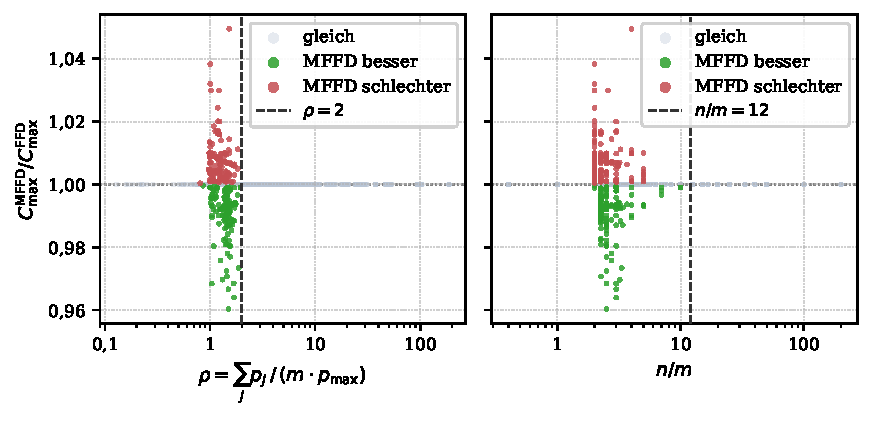
\includegraphics[width=\textwidth]{figures/abb_kollaps.pdf}
\caption{Makespan von MULTIFIT+MFFD im Verhältnis zu dem von MULTIFIT+FFD, über alle
  \EvalInstanzen{} Instanzen des Benchmarks und aufgetragen gegen
  $\rho = \sum_j p_j / (m \cdot p_{\max})$ (links) und gegen $n/m$ (rechts).
  Rechts der Linie $\rho = 2$ liegt keine Abweichung.}
\label{fig:kollaps}
\end{figure}

Tabelle~\ref{tab:kollaps} zeigt den Übergang.
Der Anteil abweichender Instanzen erreicht sein Maximum mit \EvalKollapsMaxAnteil{} im Bereich
\EvalKollapsMaxBereich{} und fällt unmittelbar unterhalb der Schwelle auf
\EvalKollapsLetzterAnteil, oberhalb von $\rho = 2$ auf null.
Die Schranke aus Lemma~\ref{lem:kollaps} ist auf diesen Datensätzen also nicht nur korrekt,
sondern wird auch fast erreicht.
Auf den \EvalRhoUnterZwei{} Instanzen mit $\rho < 2$ ist ein Unterschied möglich; wie er
ausfällt, behandelt der nächste Abschnitt.

\begin{table}[htbp]
\centering
\begin{tabular}{l r r r}
\toprule
Bereich & Instanzen & Abweichungen & Anteil \\
\midrule
$\rho < 0{,}5$ & 11 & 0 & 0{,}0\,\% \\
$0{,}5 \le \rho < 1{,}0$ & 242 & 11 & 4{,}5\,\% \\
$1{,}0 \le \rho < 1{,}25$ & 1\,790 & 140 & 7{,}8\,\% \\
$1{,}25 \le \rho < 1{,}5$ & 1\,394 & 153 & 11{,}0\,\% \\
$1{,}5 \le \rho < 1{,}75$ & 1\,253 & 68 & 5{,}4\,\% \\
$1{,}75 \le \rho < 2{,}0$ & 913 & 8 & 0{,}9\,\% \\
\midrule
$\rho \ge 2{,}0$ & \textbf{3\,489} & \textbf{0} & \textbf{0{,}0\,\%} \\
\bottomrule
\end{tabular}

\caption{Anteil der Instanzen, auf denen MULTIFIT+MFFD und MULTIFIT+FFD verschiedene Makespans
  liefern, gestaffelt nach $\rho$. Oberhalb von $\rho = 2$ tritt keine Abweichung auf
  (Lemma~\ref{lem:kollaps}).}
\label{tab:kollaps}
\end{table}

\subsection{Makespan-Vergleich}
\label{sec:makespan-vergleich}

Über alle \EvalInstanzen{} Instanzen liefert MULTIFIT+MFFD in \EvalWins{} Fällen
(\EvalWinsProzent) einen kleineren, in \EvalLosses{} Fällen (\EvalLossesProzent) einen größeren
und in \EvalTies{} Fällen (\EvalTiesProzent) denselben Makespan wie MULTIFIT+FFD
(Tabelle~\ref{tab:win-tie-loss}).
Sämtliche \EvalAbweichungen{} Abweichungen liegen bei $\rho < 2$, wie es
Lemma~\ref{lem:kollaps} verlangt.

\begin{table}[htbp]
\centering
\small
\begin{tabular}{l r r r r r r r}
\toprule
Datensatz & $N$ & MFFD besser & gleich & MFFD schlechter & \multicolumn{3}{c}{$C^{\mathrm{MFFD}}_{\max}/C^{\mathrm{FFD}}_{\max}$} \\
\cmidrule(lr){6-8}
 & & & & & Min. & Median & Max. \\
\midrule
França & 150 & 0 & 150 & 0 & 1{,}0000 & 1{,}0000 & 1{,}0000 \\
Frangioni & 780 & 1 & 775 & 4 & 0{,}9996 & 1{,}0000 & 1{,}0135 \\
Lawrinenko & 3\,499 & 146 & 3\,245 & 108 & 0{,}9603 & 1{,}0000 & 1{,}0244 \\
Berndt & 3\,059 & 17 & 3\,030 & 12 & 0{,}9667 & 1{,}0000 & 1{,}0112 \\
Planted & 1\,604 & 36 & 1\,512 & 56 & 0{,}9640 & 1{,}0000 & 1{,}0495 \\
\midrule
\textbf{Alle} & 9\,092 & 200 & 8\,712 & 180 & 0{,}9603 & 1{,}0000 & 1{,}0495 \\
\bottomrule
\end{tabular}

\caption{Vergleich der Makespans von MULTIFIT+MFFD und MULTIFIT+FFD je Datensatz. Die Zeile
  \emph{Alle} berechnet Anzahlen und Kennzahlen über alle Instanzen gemeinsam.}
\label{tab:win-tie-loss}
\end{table}

Die Abweichungen fallen in beide Richtungen aus und bleiben klein:
Das Verhältnis $C^{\mathrm{MFFD}}_{\max}/C^{\mathrm{FFD}}_{\max}$ liegt zwischen \EvalMinRatioMffdFfd{} und
\EvalMaxRatioMffdFfd{} (Abbildung~\ref{fig:ratio-verteilung}).
Auf welcher Seite sie überwiegen, hängt vom Datensatz ab: Auf Lawrinenko und Berndt liefert
MFFD häufiger den kleineren, auf Frangioni und Planted häufiger den größeren Makespan
(Tabelle~\ref{tab:win-tie-loss}).
Einen systematisch kleineren Makespan liefert MULTIFIT+MFFD auf diesen Instanzen also nicht.
Aus den Schranken~\eqref{eq:ffd-guete} und~\eqref{eq:mffd-guete} ließ sich das auch nicht
erwarten: Beide beschränken nur die Binzahl nach oben und sagen nichts über den Makespan von
MULTIFIT, und für MULTIFIT+MFFD ist keine Makespan-Schranke bewiesen.

\begin{figure}[htbp]
\centering
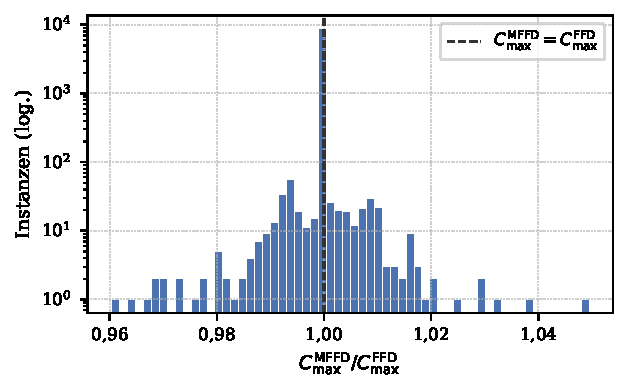
\includegraphics[width=0.72\textwidth]{figures/abb_ratio_verteilung.pdf}
\caption{Verteilung von $C^{\mathrm{MFFD}}_{\max}/C^{\mathrm{FFD}}_{\max}$ über alle \EvalInstanzen{} Instanzen
  (logarithmische $y$-Achse). Der Balken bei 1 enthält die \EvalTies{} Instanzen mit
  identischem Makespan.}
\label{fig:ratio-verteilung}
\end{figure}

\subsection{Güte gegenüber dem Optimum}
\label{sec:guete}

Auf den \EvalOptBekannt{} Instanzen mit bekanntem Optimum erreicht MULTIFIT+FFD in
\EvalOptimalFFD{} der Fälle exakt den optimalen Makespan.
Das größte beobachtete Verhältnis beträgt für beide Varianten \EvalMaxRatioOptFFD{} -
für MULTIFIT+FFD wie für MULTIFIT+MFFD -, jeweils auf einer Berndt-Instanz
(Tabelle~\ref{tab:ratio-opt}, Abbildung~\ref{fig:guete-opt}).
Beide Werte liegen unterhalb von $13/11 + 2^{-k} \approx \EvalSchrankeK$ für $k = \EvalKMax$.
Bewiesen ist diese Schranke nur für MULTIFIT+FFD, nämlich durch Theorem~\ref{thm:guete} zusammen
mit $r_m \le 13/11$ nach \textcite{cao1995}; für MULTIFIT+MFFD dient sie hier lediglich als
Vergleichslinie.

\begin{table}[htbp]
\centering
\small
\begin{tabular}{l r r r r r r r}
\toprule
Datensatz & $C^{*}_{\max}$ bekannt & \multicolumn{3}{c}{MULTIFIT+FFD} & \multicolumn{3}{c}{MULTIFIT+MFFD} \\
\cmidrule(lr){3-5}\cmidrule(lr){6-8}
 & & Mittel & Max. & $=C^{*}_{\max}$ & Mittel & Max. & $=C^{*}_{\max}$ \\
\midrule
França & 3 & 1{,}0000 & 1{,}0000 & 100{,}0\,\% & 1{,}0000 & 1{,}0000 & 100{,}0\,\% \\
Frangioni & 747 & 1{,}0066 & 1{,}0383 & 29{,}9\,\% & 1{,}0067 & 1{,}0383 & 29{,}5\,\% \\
Lawrinenko & 3\,488 & 1{,}0192 & 1{,}1080 & 27{,}5\,\% & 1{,}0190 & 1{,}1080 & 26{,}0\,\% \\
Berndt & 3\,056 & 1{,}0182 & 1{,}1221 & 19{,}1\,\% & 1{,}0181 & 1{,}1221 & 19{,}1\,\% \\
Planted & 1\,218 & 1{,}0034 & 1{,}1000 & 40{,}9\,\% & 1{,}0036 & 1{,}1000 & 40{,}1\,\% \\
\midrule
\textbf{Alle} & 8\,512 & 1{,}0154 & 1{,}1221 & 26{,}6\,\% & 1{,}0154 & 1{,}1221 & 25{,}9\,\% \\
\bottomrule
\end{tabular}

\caption{Verhältnis $C^{\mathrm{MF}}_{\max}/C^{*}_{\max}$ über die \EvalOptBekannt{} Instanzen mit
  bekanntem Optimum. \emph{Mittel} ist das arithmetische Mittel über die Instanzen, die Spalte
  $=C^{*}_{\max}$ gibt den Anteil der Instanzen an, auf denen MULTIFIT den optimalen Makespan
  erreicht. Die Zeile \emph{Alle} berechnet dieselben Kennzahlen über alle Instanzen
  gemeinsam.}
\label{tab:ratio-opt}
\end{table}

\begin{figure}[htbp]
\centering
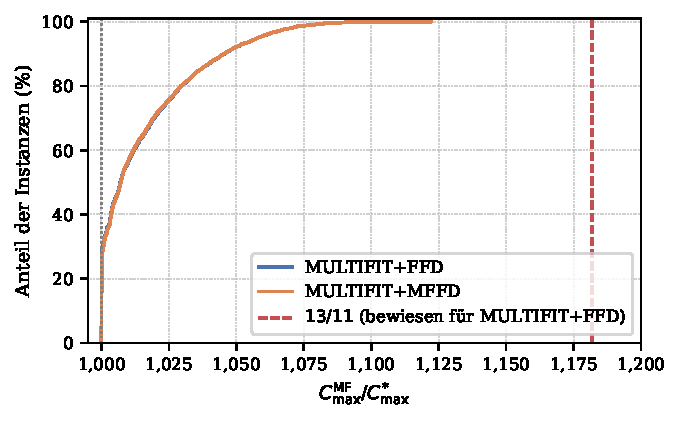
\includegraphics[width=0.78\textwidth]{figures/abb_guete_opt.pdf}
\caption{Empirische Verteilungsfunktion von $C^{\mathrm{MF}}_{\max}/C^{*}_{\max}$ über die
  \EvalOptBekannt{} Instanzen mit bekanntem Optimum. Die gestrichelte Linie markiert $13/11$;
  als Schranke bewiesen ist dieser Wert nur für MULTIFIT+FFD.}
\label{fig:guete-opt}
\end{figure}

Für die \EvalOhneOpt{} Instanzen ohne bekanntes Optimum lässt sich dieselbe Aussage über die
untere Schranke aus \eqref{eq:lb} führen: Aus $\mathrm{LB} \le C^{*}_{\max}$ folgt
$C^{\mathrm{MF}}_{\max}/C^{*}_{\max} \le C^{\mathrm{MF}}_{\max}/\mathrm{LB}$.
Auf allen \EvalLbBelegt{} dieser Instanzen gilt $C^{\mathrm{MF}}_{\max}/\mathrm{LB} \le \EvalMaxRatioLb$
und damit erst recht $C^{\mathrm{MF}}_{\max}/C^{*}_{\max} \le 13/11$
(Tabelle~\ref{tab:abdeckung}).

\begin{table}[htbp]
\centering
\begin{tabular}{l r r r r}
\toprule
Datensatz & $N$ & $C^{*}_{\max}$ bekannt & über $\mathrm{LB}$ belegt & unbestimmt \\
\midrule
França & 150 & 3 & 147 & 0 \\
Frangioni & 780 & 747 & 33 & 0 \\
Lawrinenko & 3\,499 & 3\,488 & 11 & 0 \\
Berndt & 3\,059 & 3\,056 & 3 & 0 \\
Planted & 1\,604 & 1\,218 & 386 & 0 \\
\midrule
\textbf{Gesamt} & 9\,092 & 8\,512 & 580 & 0 \\
\bottomrule
\end{tabular}

\caption{Abdeckung der gemessenen Aussage $C^{\mathrm{MF}}_{\max}/C^{*}_{\max} \le 13/11$ für
  MULTIFIT+FFD und MULTIFIT+MFFD. Für Instanzen ohne bekanntes Optimum wird sie über die untere
  Schranke~\eqref{eq:lb} belegt.}
\label{tab:abdeckung}
\end{table}

Damit gilt für jede der \EvalInstanzen{} Instanzen, dass weder MULTIFIT+FFD noch
MULTIFIT+MFFD das Verhältnis $13/11$ überschreitet; der größte über alle Instanzen mit bekanntem Optimum
gemessene Wert ist \EvalMaxRatioOpt.
Das ist eine Aussage über diese Instanzmenge: Für MULTIFIT+FFD ist sie mit der bewiesenen
Schranke verträglich, für MULTIFIT+MFFD begründet sie keine.
Die Worst-Case-Instanz von \textcite{friesen1984}, auf der MULTIFIT+FFD das Verhältnis $13/11$
exakt annimmt, ist in keinem der fünf Datensätze enthalten; Abschnitt~\ref{sec:friesen} wertet
sie deshalb gesondert für beide Subroutinen aus.

\subsection{Laufzeit}
\label{sec:laufzeit}

MFFDs zusätzliche Klassifikation kostet Laufzeit.
Der Median des instanzweisen Verhältnisses $t_{\mathrm{MFFD}}/t_{\mathrm{FFD}}$
liegt je nach Datensatz zwischen \EvalZeitMedianMin{} und
\EvalZeitMedianMax{} (Tabelle~\ref{tab:laufzeit}, Abbildung~\ref{fig:laufzeit} links).
Der Mehraufwand ist damit messbar, bleibt aber ein konstanter Faktor.

\begin{table}[htbp]
\centering
\begin{tabular}{l r r r r}
\toprule
Datensatz & Median FFD & Median MFFD & \multicolumn{2}{c}{$t_{\mathrm{MFFD}}/t_{\mathrm{FFD}}$} \\
\cmidrule(lr){4-5}
 & (ms) & (ms) & Median & 95.\ Perzentil \\
\midrule
França & 1{,}600 & 1{,}982 & 1{,}201 & 1{,}837 \\
Frangioni & 1{,}630 & 2{,}000 & 1{,}173 & 1{,}646 \\
Lawrinenko & 2{,}010 & 1{,}952 & 1{,}037 & 1{,}374 \\
Berndt & 0{,}339 & 0{,}498 & 1{,}522 & 2{,}078 \\
Planted & 1{,}743 & 2{,}027 & 1{,}154 & 1{,}855 \\
\midrule
\textbf{Alle} & 1{,}051 & 1{,}095 & 1{,}217 & 1{,}965 \\
\bottomrule
\end{tabular}

\caption{Laufzeit eines vollständigen MULTIFIT-Laufs ($k = 10$) und paarweises Verhältnis
  beider Subroutinen je Instanz. Die Zeile \emph{Alle} gibt Median und Perzentil über
  alle Instanzen gemeinsam an, nicht einen Mittelwert der Datensatzzeilen.}
\label{tab:laufzeit}
\end{table}

\begin{figure}[htbp]
\centering
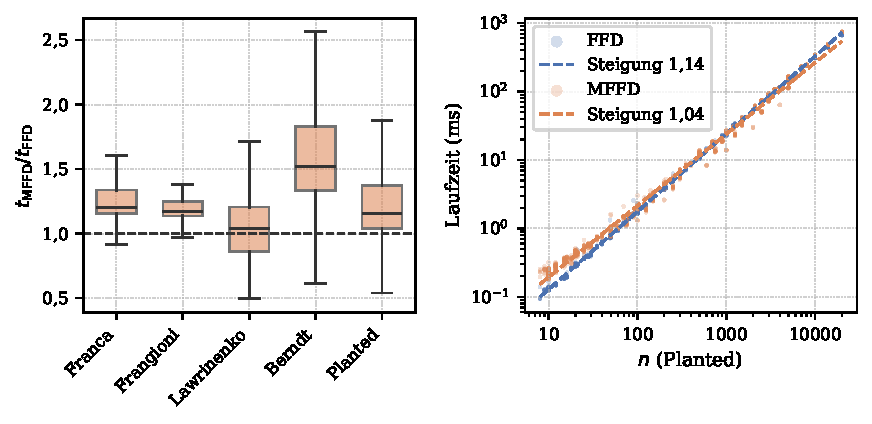
\includegraphics[width=\textwidth]{figures/abb_laufzeit.pdf}
\caption{Links: paarweises Laufzeitverhältnis je Datensatz (ohne Ausreißer).
  Rechts: Laufzeit gegen $n$ auf dem Planted-Datensatz, dessen $n$ sich über drei
  Größenordnungen erstreckt, mit Ausgleichsgeraden im doppelt-logarithmischen Maßstab.}
\label{fig:laufzeit}
\end{figure}

Das Wachstum in $n$ unterscheidet sich zwischen beiden Subroutinen nicht wesentlich:
Auf dem Planted-Datensatz, dem einzigen mit einem $n$-Bereich über drei Größenordnungen,
beträgt die Steigung der Ausgleichsgeraden im doppelt-logarithmischen Maßstab
\EvalSteigungFFD{} für FFD und \EvalSteigungMFFD{} für MFFD
(Abbildung~\ref{fig:laufzeit} rechts).
Eine Steigung nahe 1 ist mit der Laufzeit $O(n \log n)$ beider Implementierungen verträglich.
Zur Einordnung der absoluten Werte siehe Abschnitt~\ref{sec:grenzen}.

\subsection{Sensitivität gegenüber der Binärsuchtiefe}
\label{sec:k-sensitivitaet}

Nach Theorem~\ref{thm:guete} gilt für MULTIFIT+FFD $R_m(\mathrm{MF}(k)) \le r_m + 2^{-k}$: Der
additive Term, welcher auf die Binärsuche entfällt, halbiert sich mit jedem Halbierungsschritt.
Um zu messen, ab welchem $k$ sich das Ergebnis auf den Benchmark-Instanzen nicht mehr ändert,
wurde MULTIFIT für $k = 1, \ldots, 10$ über alle \EvalInstanzen{} Instanzen ausgeführt.

Das gemessene Maximum liegt für beide Subroutinen bei jeder Tiefe unterhalb von
$13/11 + 2^{-k}$, der für MULTIFIT+FFD bewiesenen Schranke
(Tabelle~\ref{tab:k-sensitivitaet}, Abbildung~\ref{fig:k-sensitivitaet} rechts):
bei $k = 1$ sind es \EvalKMaxEins{} gegenüber \EvalKSchrankeEins{}, bei
$k = \EvalKStabilMax$ dann \EvalKMaxZehn{} gegenüber \EvalKSchrankeStabil{} und bei
$k = \EvalKMax$ \EvalKMaxZehn{} gegenüber \EvalSchrankeK.

\begin{figure}[htbp]
\centering
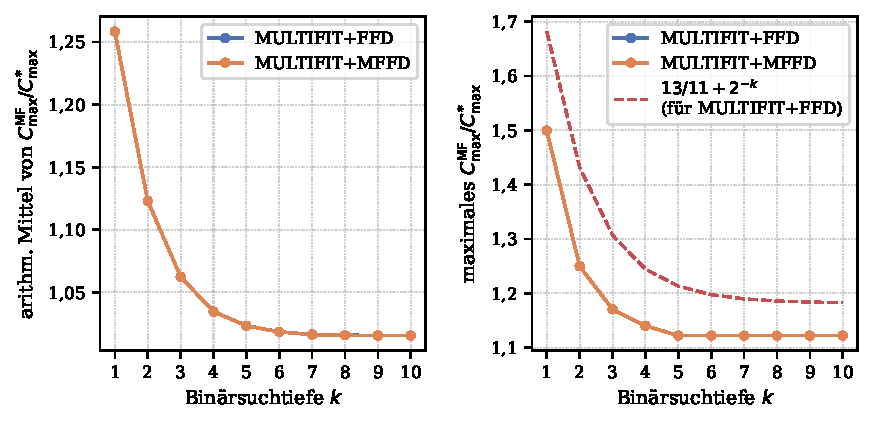
\includegraphics[width=\textwidth]{figures/abb_k_sensitivitaet.pdf}
\caption{Arithmetisches Mittel (links) und Maximum (rechts) des Verhältnisses
  $C^{\mathrm{MF}}_{\max}/C^{*}_{\max}$ in Abhängigkeit der Binärsuchtiefe $k$ über die
  \EvalOptBekannt{} Instanzen mit bekanntem Optimum. Rechts zusätzlich die für MULTIFIT+FFD
  bewiesene Schranke $13/11 + 2^{-k}$ nach \textcite{cao1995}.}
\label{fig:k-sensitivitaet}
\end{figure}
Ab $k = \EvalKStabilMax$ ändert sich das Maximum nicht mehr; der Mittelwert sinkt dagegen
bis $k = \EvalKMax$ weiter, von \EvalKMittelEins{} bei $k = 1$ auf \EvalKMittelZehn.

\begin{table}[htbp]
\centering
\small
\begin{tabular}{r r r r r r r}
\toprule
$k$ & \multicolumn{2}{c}{MULTIFIT+FFD} & \multicolumn{2}{c}{MULTIFIT+MFFD} & $13/11 + 2^{-k}$ & stabil \\
\cmidrule(lr){2-3}\cmidrule(lr){4-5}
 & Mittel & Max. & Mittel & Max. & & \\
\midrule
1 & 1{,}2584 & 1{,}4997 & 1{,}2584 & 1{,}4997 & 1{,}6818 & 0{,}2\,\% \\
2 & 1{,}1230 & 1{,}2497 & 1{,}1230 & 1{,}2497 & 1{,}4318 & 1{,}9\,\% \\
3 & 1{,}0624 & 1{,}1705 & 1{,}0624 & 1{,}1705 & 1{,}3068 & 6{,}3\,\% \\
4 & 1{,}0346 & 1{,}1400 & 1{,}0345 & 1{,}1400 & 1{,}2443 & 14{,}6\,\% \\
5 & 1{,}0233 & 1{,}1221 & 1{,}0232 & 1{,}1221 & 1{,}2131 & 27{,}7\,\% \\
6 & 1{,}0184 & 1{,}1221 & 1{,}0183 & 1{,}1221 & 1{,}1974 & 48{,}0\,\% \\
7 & 1{,}0163 & 1{,}1221 & 1{,}0162 & 1{,}1221 & 1{,}1896 & 69{,}6\,\% \\
8 & 1{,}0157 & 1{,}1221 & 1{,}0156 & 1{,}1221 & 1{,}1857 & 83{,}1\,\% \\
9 & 1{,}0155 & 1{,}1221 & 1{,}0155 & 1{,}1221 & 1{,}1838 & 91{,}5\,\% \\
10 & 1{,}0154 & 1{,}1221 & 1{,}0154 & 1{,}1221 & 1{,}1828 & 100{,}0\,\% \\
\bottomrule
\end{tabular}

\caption{Verhältnis $C^{\mathrm{MF}}_{\max}/C^{*}_{\max}$ in Abhängigkeit der Binärsuchtiefe $k$
  über die \EvalOptBekannt{} Instanzen mit bekanntem Optimum. \emph{Mittel} ist das
  arithmetische Mittel, $13/11 + 2^{-k}$ die für MULTIFIT+FFD bewiesene Schranke.
  Die letzte Spalte gibt den Anteil der Instanzen an, auf denen MULTIFIT+FFD bei $k$ bereits
  denselben Makespan liefert wie bei $k = \EvalKMax$ (die letzte Zeile daher definitionsgemäß
  $100\,\%$).}
\label{tab:k-sensitivitaet}
\end{table}

Auch bei $k = \EvalKMax$ hat sich der Makespan nicht auf allen Instanzen stabilisiert: Bei
MULTIFIT+FFD stimmt er auf \EvalKStabilNeun{} der Instanzen bei $k = 9$ mit dem bei
$k = \EvalKMax$ überein, auf den übrigen ändert er sich im letzten Halbierungsschritt noch.
Da die Suche reellwertige Kapazitäten testet, schrumpft das Suchintervall mit jedem Schritt,
wird aber nie leer; ein größeres $k$ kann folglich eine noch kleinere akzeptierte Kapazität und
damit einen kleineren Makespan liefern.
Die ganzzahlige Suche aus Abschnitt~\ref{sec:hm} endet dagegen, sobald sich untere und obere
Grenze des Intervalls treffen.

Der Makespan fällt allerdings nicht durchgängig monoton in $k$.
MULTIFIT verkleinert die Kapazitätsschranke $C$, nicht den tatsächlich erreichten Makespan:
Passt eine Packung mit kleinerem $C$ noch in $m$ Bins, wird sie übernommen, auch wenn ihre
größte Binlast über der der bisher gespeicherten Packung liegt.
Über alle \EvalInstanzen{} Instanzen und alle Übergänge $k \to k+1$ zählt die Messung
\EvalKNichtMonotonFFD{} solche Fälle bei MULTIFIT+FFD und \EvalKNichtMonotonMFFD{} bei
MULTIFIT+MFFD; die größte dabei gemessene Verschlechterung beträgt \EvalKNichtMonotonMax{}
(Instanz \texttt{\EvalKNichtMonotonInstanz}: Makespan \EvalKNichtMonotonVorher{} bei
$k = \EvalKNichtMonotonKVorher$, \EvalKNichtMonotonNachher{} bei
$k = \EvalKNichtMonotonKNachher$, gemessen mit \EvalKNichtMonotonAlg).


\subsection{Fallstudie: die Friesen-Instanz}
\label{sec:friesen}

Keine Instanz der fünf Datensätze erreicht das Verhältnis $13/11$.
Die von \textcite{friesen1984} angegebene Instanz, auf der MULTIFIT+FFD diesen Wert
annimmt, erlaubt es, das Verhalten beider Subroutinen an einem Extremfall nachzuvollziehen.

Die Instanz besteht aus $n = 39$ Aufgaben auf $m = 13$ Maschinen:
achtmal $(40, 13, 13)$, dreimal $(25, 25, 16)$ und zweimal $(25, 24, 17)$.
Die Gesamtlast ist $858 = 13 \cdot 66$, und es existiert eine Zuordnung, bei der jede Maschine
exakt 66 Lasteinheiten erhält; also $C^{*}_{\max} = 66$.
Wegen $\rho = 858 / (13 \cdot 40) = 1{,}65 < 2$ dürfen sich die Subroutinen nach
Lemma~\ref{lem:kollaps} unterscheiden - und sie tun es:

\begin{center}
\begin{tabular}{l r r}
\toprule
 & MULTIFIT+FFD & MULTIFIT+MFFD \\
\midrule
Makespan ($k = 10$)        & 78     & 75 \\
Verhältnis zu $C^{*}_{\max}$ & $78/66 = 13/11$ & $75/66 \approx 1{,}1364$ \\
\bottomrule
\end{tabular}
\end{center}

Der Unterschied entsteht bei der Kapazität $C = 75$.
Dort ist $C/2 = 37{,}5$, sodass die acht 40er-Aufgaben \emph{large} sind, und $C/6 = 12{,}5$,
sodass auch die 13er-Aufgaben noch \emph{small} sind.
Phase~3 von MFFD kombiniert daher jeden 40er-Bin mit einer 13er-Aufgabe und einer weiteren
passenden Aufgabe; MFFD packt die Instanz in 13~Bins, FFD benötigt 14.
Bei $C = 78$ dagegen ist $C/6 = 13$ und die 13er-Aufgaben sind \emph{tiny};
Phase~3 bleibt für sie wirkungslos.

Abbildung~\ref{fig:friesen-binzahl} zeigt die Binzahlen beider Subroutinen für jede ganzzahlige
Kapazität von $C^{*}_{\max} = 66$ bis $90$.
FFD benötigt für jede Kapazität von 66 bis 77 vierzehn Bins und fällt bei $C = 78$ auf elf;
die Binärsuche akzeptiert daher erst $C = 78$.
MFFD kommt bereits ab $C = 75$ mit 13~Bins aus, weshalb MULTIFIT+MFFD gegen 75 konvergiert.
Erreicht wird dieser Wert ab $k \ge 6$; bei kleinerem $k$ liegt das Suchintervall noch zu grob
(bei $k = 5$ ergibt sich 76).

\begin{figure}[htbp]
\centering
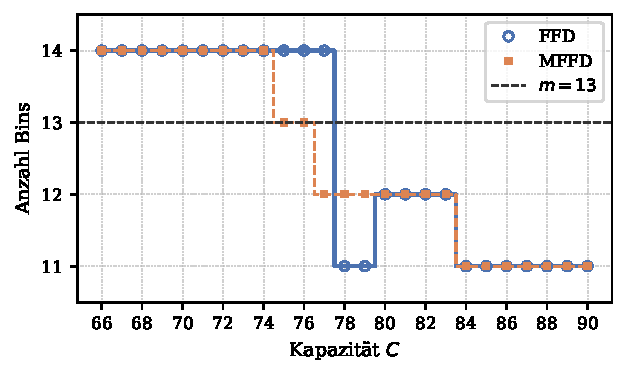
\includegraphics[width=0.72\textwidth]{figures/abb_friesen_binzahl.pdf}
\caption{Anzahl der Bins von FFD und MFFD auf der Friesen-Instanz für jede ganzzahlige Kapazität
  $C = 66, \ldots, 90$. MULTIFIT akzeptiert eine Kapazität, wenn die Binzahl auf oder unter der
  gestrichelten Linie $m = 13$ liegt. Beim Übergang von $C = 79$ auf $C = 80$ steigt die Binzahl
  von FFD.}
\label{fig:friesen-binzahl}
\end{figure}

Der Übergang von $C = 79$ auf $C = 80$ belegt zugleich, dass die Binzahl von FFD nicht monoton
in $C$ fällt.
Bei $C = 79$ kombiniert First Fit jede 40er-Aufgabe mit einer 25er- und einer 13er-Aufgabe zur
Last 78 und füllt so elf Bins.
Bei $C = 80$ passen zwei 40er-Aufgaben gemeinsam in einen Bin; dadurch entfällt diese
Kombination, die 25er-Aufgaben belegen eigene Bins, und am Ende bleibt eine 13er-Aufgabe
allein in einem zwölften Bin.
Erst ab $C = 84$ kommt FFD wieder mit elf Bins aus.
Auf dieser Instanz bleibt das ohne Folgen für MULTIFIT, da beide Werte unter $m = 13$ liegen und
das Akzeptanzkriterium $\mathrm{FFD}[\Gamma, C] \le m$ damit in beiden Fällen erfüllt ist.

Dass MULTIFIT+MFFD auf dieser Instanz besser abschneidet, sagt nichts über sein
Worst-Case-Verhältnis aus.
Ob $r_m(\mathrm{MF{+}MFFD}) < 13/11$ gilt, ist offen.

\subsection{Grenzen der Auswertung}
\label{sec:grenzen}

\begin{itemize}
  \item \textbf{Herkunft der Optima.} Die OPT-Werte für Frangioni, Lawrinenko, Berndt und einen
    Teil der Planted-Instanzen stammen aus \textcite{akram2025} und wurden nicht selbst
    nachgerechnet. Sie gehen in Abschnitt~\ref{sec:guete} unmittelbar in das Verhältnis
    $C^{\mathrm{MF}}_{\max}/C^{*}_{\max}$ ein. Die über \eqref{eq:lb} geführte Argumentation ist davon
    unabhängig.
  \item \textbf{Laufzeitmessung.} Jede Instanz wurde einmal gemessen. Die Werte in
    Tabelle~\ref{tab:laufzeit} sind Mediane über viele Instanzen, aber keine Mittel über
    wiederholte Läufe derselben Instanz; einzelne Werte enthalten Messrauschen.
    Die absoluten Zeiten gelten für die beschriebene Python-Implementierung und Umgebung.
  \item \textbf{Abdeckung des Parameterraums.} \EvalRhoZweiProzent{} der Instanzen erfüllen
    $\rho \ge 2$ und sind nach Lemma~\ref{lem:kollaps} für den Subroutinenvergleich ohne
    Aussagekraft. Die verbleibenden \EvalRhoUnterZwei{} Instanzen konzentrieren sich auf
    $\rho \in [1;\,2]$; sehr kleine Werte $\rho < 0{,}5$ kommen nur elfmal vor.
  \item \textbf{Reichweite der Ergebnisse.} Alle Angaben beziehen sich auf $k = 10$ und auf
    diese fünf Datensätze. Aus dem Ausbleiben eines Verhältnisses über $13/11$ folgt keine
    schärfere Schranke, und aus den beobachteten Abweichungen folgt keine Aussage über das
    Worst-Case-Verhalten von MULTIFIT+MFFD.
\end{itemize}

\section{High-Multiplicity-Subroutinen}
\label{sec:hm}

Kommen in einer Instanz nur $d$ verschiedene Aufgabengrößen vor, lässt sie sich kompakter
kodieren: Statt der $n$ einzelnen Größen genügen die verschiedenen Größen $p_1, \ldots, p_d$ und
ihre Vielfachheiten $u_1, \ldots, u_d$ (High-Multiplicity-Darstellung,
Abschnitt~\ref{sec:jansen}).
Die Kodierungslänge liegt dann in $O\bigl(d \cdot (\log p_{\max} + \log n)\bigr)$, während die
Liste der Aufgabengrößen $n$ Zahlen umfasst.
Erst in dieser Kodierung ist eine Laufzeit polynomiell in $\log n$, wie sie
Abschnitt~\ref{sub:jansen-laufzeit} angibt, überhaupt möglich, denn schon das Einlesen von $n$
einzelnen Größen kostet $\Omega(n)$.
Kapitel~\ref{kap:alternative} stellt neben MFFD drei Subroutinen vor, welche diese Darstellung
ausnutzen: den $\mathrm{OPT}+1$-Algorithmus von \textcite{jansen_solisoba2010}
(Abschnitt~\ref{sec:jansen}), seine $\varepsilon$-duale Modifikation
(Abschnitt~\ref{sub:eps_dual}) und das Konfigurations-LP von Gilmore und Gomory
(Abschnitt~\ref{sec:gg-lp}).
Dieser Abschnitt misst, was sie als Subroutine in MULTIFIT leisten.

Gegenüber Abschnitt~\ref{sec:greedy} kommt dabei ein Hilfsmittel hinzu: Dasselbe
Konfigurationsprogramm liefert in ganzzahliger Fassung $\mathrm{OPT}[\Gamma, C]$ exakt.
Bei jeder getesteten Kapazität ist damit bekannt, wie viele Bins mindestens nötig sind -
die Schranken aus Kapitel~\ref{kap:alternative} lassen sich nachrechnen, statt sie nur zu
zitieren.

\subsection{Datensätze}
\label{sub:hm-datensaetze}

Die fünf Datensätze aus Abschnitt~\ref{sec:benchmarks} sind für diesen Vergleich ungeeignet:
Ihre Instanzen enthalten im Median zwischen \HmDBenchMedianMin{} und \HmDBenchMedianMax{}
verschiedene Aufgabengrößen, im Maximum \HmDBenchMax.
Nach Abschnitt~\ref{sub:anwendbarkeit} setzen die Verfahren ein konstantes und sehr kleines $d$
voraus.
Für den Vergleich wurden deshalb zwei Datensätze erzeugt.

\paragraph{HM-Gitter.}
Der erste Datensatz - HM steht für High Multiplicity - umfasst
\HmInstanzen{} Instanzen aus einem vollständig balancierten Gitter:
$d \in \{\HmDMin,\dots,\HmDMax\}$ verschiedene Aufgabengrößen, drei Szenarien für deren
Verteilung, drei Maschinenzahlen zwischen \HmMMin{} und \HmMMax{} und drei Verhältnisse $n/m$
mit je zehn Instanzen (Tabelle~\ref{tab:hm-datensatz}).
Die Größenbereiche sind aus $\varepsilon = 1/(2d-1)$ abgeleitet, also aus der
Groß-Klein-Schwelle des $\mathrm{OPT}+1$-Algorithmus selbst.
Die Instanzen sind klein ($n$ zwischen \HmNMin{} und \HmNMax); variiert werden $d$, $m$ und
$n/m$, nicht die Vielfachheiten.

\begin{table}[htbp]
\centering
\begin{tabular}{lrrrrr}
\toprule
Szenario & Instanzen & $n$ & $m$ & $d$ & $\rho$ \\
\midrule
Dense & 360 & 15--160 & 5--20 & 3--6 & 1{,}34--7{,}74 \\
Mixed & 360 & 15--160 & 5--20 & 3--6 & 0{,}52--7{,}74 \\
Asymmetric & 360 & 15--160 & 5--20 & 3--6 & 0{,}67--7{,}00 \\
\midrule
Gesamt & 1\,080 & 15--160 & 5--20 & 3--6 & 0{,}52--7{,}74 \\
\bottomrule
\end{tabular}

\caption{Aufbau des HM-Gitters. Je Szenario \HmInstanzenSzenario{} Instanzen aus
  $d \in \{\HmDMin,\dots,\HmDMax\}$, drei Maschinenzahlen, drei Verhältnissen $n/m$ und zehn
  Instanzen je Kombination.}
\label{tab:hm-datensatz}
\end{table}

\paragraph{HM-Skalierung.}
\HmSkalInstanzen{} Instanzen, die die fehlende Achse ergänzen: $d \in \{3,4\}$, dieselben drei
Szenarien, $n$ von \HmSkalNMin{} bis \HmSkalNMax{} bei festem $n/m = \HmSkalRatio$ (also $m$ bis
\HmSkalMMax), je fünf Instanzen.
Das feste Verhältnis ist konstruktionsbedingt nötig: Bei festem $m$ wüchse mit $n$ auch das
Startintervall der Binärsuche~\eqref{eq:startintervall} und mit ihm die Zahl der
Konfigurationen; bei festem $n/m$ bleibt die getestete Kapazität in derselben Größenordnung, und
es wachsen allein die Vielfachheiten.
Damit ein Konfigurations-LP je Kapazität lösbar bleibt, verwirft der Generator jede
Größenkombination, bei welcher die obere Schranke $\prod_{i=1}^{d} (\lfloor C/p_i \rfloor + 1)$ für die
Zahl der Konfigurationen über \HmSkalBudget{} liegt.
Dabei ist $C = \HmSkalRatio\,\bar{p} + p_{\max}$ mit dem Mittelwert $\bar{p}$ der $d$ Größen,
eine von $n$ unabhängige Näherung der oberen Grenze des Startintervalls.
Diese Grenze beschränkt $d$: Schon für $d = \HmSkalDLuecke$ hält im Szenario
\HmSkalSzenarioLuecke{} keine von \HmSkalZuege{} zufällig gezogenen Größenkombinationen sie ein,
während für $d \le \HmSkalDMaxAlle$ in allen drei Szenarien zulässige Kombinationen existieren.
Dieser Datensatz wird nur in Abschnitt~\ref{sub:hm-skalierung} ausgewertet.

\paragraph{Referenzwerte.}
Für alle \HmInstanzen{} Instanzen des HM-Gitters wurde $C^{*}_{\max}(\Gamma)$ für diese Arbeit
exakt bestimmt.
Nach Lemma~\ref{lem:dualitaet} ist
$C^{*}_{\max}(\Gamma) = \min\{C : \mathrm{OPT}[\Gamma, C] \le m\}$, und da
$\mathrm{OPT}[\Gamma,\cdot\,]$ monoton fällt, findet eine Binärsuche über $C$ diesen Wert,
sobald sich $\mathrm{OPT}[\Gamma, C]$ berechnen lässt.
Das leistet das ganzzahlige Konfigurationsprogramm; seine Größe hängt nur von $d$ und $C$ ab,
nicht von $n$ oder $m$.
Alle \HmInstanzen{} Werte sind auf diesem Weg als optimal nachgewiesen.

\paragraph{Degenerierte Instanzen.}
\HmDegeneriert{} Instanzen des HM-Gitters erfüllen $\rho(\Gamma) < 1$, bei ihnen übersteigt die
größte Aufgabe also die mittlere Maschinenlast; bei \HmDegOptPMax{} von ihnen ist
$C^{*}_{\max}(\Gamma) = p_{\max}$, die untere Schranke aus Lemma~\ref{lem:untere-schranken} wird
dort angenommen.
Auf diesen Instanzen erreichen \HmDegAlleOptimal{} fünf Subroutinen den optimalen Makespan; sie
trennen die Verfahren nicht und bleiben in den Gütevergleichen unberücksichtigt.

\subsection{Versuchsaufbau}
\label{sub:hm-aufbau}

\paragraph{Subroutinen.}
Gemessen werden fünf Subroutinen: FFD als Grundlinie, der $\mathrm{OPT}+1$-Algorithmus ($\mathrm{J}$), seine
$\varepsilon$-duale Variante ($\mathrm{J}_\varepsilon$), das Konfigurations-LP mit Rundung
($\mathrm{GG}$) und dasselbe Programm in ganzzahliger Fassung ($\mathrm{GG}$-IP).
Letzteres löst $\mathrm{OPT}[\Gamma, C]$ exakt und dient als Referenzlinie.

\paragraph{Implementierungsvarianten der beiden Jansen-Algorithmen.}
$\mathrm{J}$ und $\mathrm{J}_\varepsilon$ unterscheiden sich nicht nur im Rundungsschritt,
sondern auch in der Anzahl der Aufrufe des Lösers.
Für die Laufzeitmessung in Abschnitt~\ref{sub:hm-laufzeit} ist das der entscheidende
Unterschied.
$\mathrm{J}$ wird in der publizierten Form gemessen.
Schritt~2 bestimmt dort das kleinste $m^*$, für welches das MILP zulässig ist, per Binärsuche über
$\{1, \ldots, n\}$ (Abschnitt~\ref{sub:jansen-implementierung}); jeder Suchschritt löst ein MILP
und halbiert das Intervall, sodass je Kapazität $O(\log n)$ MILP-Aufrufe anfallen.
Nötig ist diese Suche, obwohl MULTIFIT die Maschinenzahl $m$ vorgibt: Ein einzelner Aufruf mit
$m$ an Stelle von $m^*$ kann wegen des zusätzlichen Bins aus Schritt~3 insgesamt $m+1$ Bins
ausgeben und die Kapazität verwerfen, obwohl die publizierte Form mit $m^* < m$ höchstens $m$
Bins ausgibt und sie annimmt (Abschnitt~\ref{sub:eps_dual}).
$\mathrm{J}_\varepsilon$ verteilt die Reste dagegen auf die bereits geöffneten Bins und wird
deshalb in der Fassung aus Abschnitt~\ref{sub:eps_dual} ohne innere Binärsuche gemessen: Je
Kapazität wird das MILP einmal mit der Nebenbedingung $\sum_b y_b \le m$ gelöst.

\paragraph{Parameter.}
Alle fünf Subroutinen laufen mit $k = 10$ wie in Abschnitt~\ref{sec:versuchsaufbau}, aber mit
\emph{ganzzahligen} Kapazitäten.
Da alle Aufgabengrößen ganzzahlig sind, ist jede Binlast ganzzahlig; eine Kapazität $C$ lässt
daher dieselben Packungen zu wie $\lfloor C \rfloor$.
Die Binärsuche testet deshalb nur ganze Zahlen, setzt nach einer Ablehnung von $C$ die untere
Grenze auf $C+1$ und endet, sobald sich untere und obere Grenze treffen.
So prüft jeder Aufruf der Subroutine eine andere Kapazität.
FFD wird deshalb in dieser Variante neu gemessen und nicht aus Abschnitt~\ref{sec:laufzeit}
übernommen.
Jede Instanz wird von allen fünf Subroutinen im selben Prozess bearbeitet.

\paragraph{Messumgebung.}
Umgebung wie in Abschnitt~\ref{sec:versuchsaufbau}; die vier übrigen Subroutinen lösen ihre
Programme mit Gurobi~13.0.2.
Die Laufzeit umfasst den vollständigen Lauf von MULTIFIT einschließlich aller Aufrufe des
Lösers, nicht einzelne Packvorgänge.

\paragraph{Reproduktion.}
Die Messung übernimmt \texttt{run\_hm\_benchmark.py} und legt zwei Dateien ab: eine Zeile je
Instanz mit Makespan und Laufzeit jeder Subroutine sowie eine Zeile je Tripel aus Instanz,
getesteter Kapazität und Subroutine mit den Kennzahlen des jeweiligen Aufrufs.
Daraus erzeugen \texttt{summary\_tables\_hm.py} die Tabellen und Kennzahlen sowie
\texttt{thesis\_figures\_hm.py} die Abbildungen.
Diese Kette ist von der aus Abschnitt~\ref{sec:versuchsaufbau} getrennt.

\subsection{Güte gegenüber dem Optimum}
\label{sub:hm-guete}

Tabelle~\ref{tab:hm-ratio-opt} und Abbildung~\ref{fig:hm-guete} zeigen den Abstand zum Optimum.
MULTIFIT+FFD erreicht auf \HmOptimalffd{} der Instanzen den optimalen Makespan, im schlechtesten
Fall das Verhältnis \HmMaxRatioOptffd.
Die drei High-Multiplicity-Subroutinen liegen darüber: \HmOptimaljansen{} für $\mathrm{J}$,
\HmOptimaljansendual{} für $\mathrm{J}_\varepsilon$ und \HmOptimalgglp{} für $\mathrm{GG}$; ihre
größten Verhältnisse liegen zwischen \HmMaxRatioOptjansendual{} und \HmMaxRatioOptjansen.

\begin{table}[htbp]
\centering
\small
\begin{tabular}{lrrrrrr}
\toprule
& & \multicolumn{5}{c}{Maximum von $C^{\mathrm{MF}}_{\max}/C^{*}_{\max}$} \\
\cmidrule(lr){3-7}
$d$ & Instanzen & FFD & Jansen OPT+1 & Jansen $\varepsilon$-dual & GG-LP & GG-IP (exakt) \\
\midrule
3 & 270 & 1{,}1429 & 1{,}0317 & 1{,}0303 & 1{,}0303 & 1{,}0000 \\
4 & 271 & 1{,}1327 & 1{,}0292 & 1{,}0216 & 1{,}0254 & 1{,}0000 \\
5 & 259 & 1{,}0920 & 1{,}0247 & 1{,}0232 & 1{,}0296 & 1{,}0000 \\
6 & 256 & 1{,}1154 & 1{,}0116 & 1{,}0217 & 1{,}0317 & 1{,}0000 \\
\midrule
alle $d$ & 1\,056 & 1{,}1429 & 1{,}0317 & 1{,}0303 & 1{,}0317 & 1{,}0000 \\
\bottomrule
\end{tabular}

\caption{Größtes Verhältnis $C^{\mathrm{MF}}_{\max}/C^{*}_{\max}$ je Subroutine, gestaffelt nach der
  Anzahl $d$ verschiedener Aufgabengrößen. Die \HmDegeneriert{} Instanzen mit $\rho < 1$ sind
  ausgenommen.}
\label{tab:hm-ratio-opt}
\end{table}

\begin{figure}[htbp]
\centering
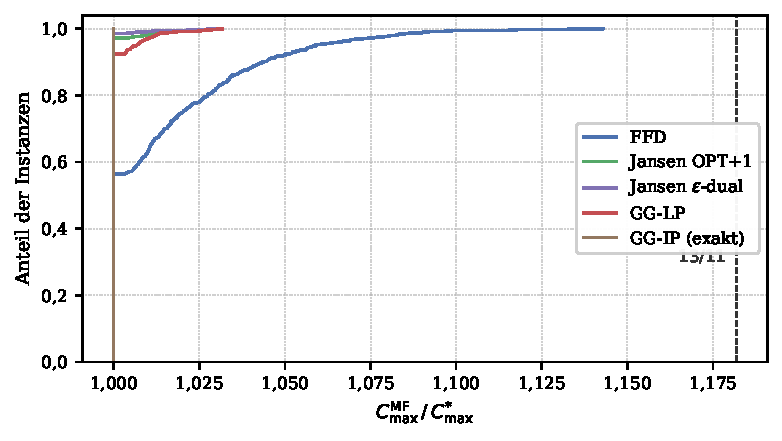
\includegraphics[width=0.90\textwidth]{figures/abb_hm_guete.pdf}
\caption{Empirische Verteilungsfunktion von $C^{\mathrm{MF}}_{\max}/C^{*}_{\max}$ je Subroutine.
  Die Verteilung von GG-IP liegt konstruktionsbedingt vollständig bei 1.}
\label{fig:hm-guete}
\end{figure}

Die Spalten der vier nicht exakten Subroutinen sind dabei unterschiedlich zu lesen.
Zwei von ihnen prüfen je eine bewiesene, instanzunabhängige Schranke nach: die Spalte zu
MULTIFIT+FFD den Wert $13/11 + 2^{-k} \approx \HmSchrankeK$ nach \textcite{cao1995}, die
Spalte zu MULTIFIT+$\mathrm{J}_\varepsilon$ den Wert $(1+\varepsilon)(1+2^{-k})$ nach
Korollar~\ref{kor:multifit-jansen-dual}, wobei $\varepsilon = 1/(2d-1)$ hier zwischen
\HmEpsTheorieMin{} und \HmEpsTheorieMax{} liegt.
Für MULTIFIT+$\mathrm{J}$ beziffert Abschnitt~\ref{sub:anwendbarkeit} die Güte durch den
Quotienten $C^{*}_{\max}(\Gamma, m-1)/C^{*}_{\max}(\Gamma, m)$, der im Allgemeinen bis
zu $2$ betragen kann - eine Schranke, die von der Instanz abhängt.
Für das Konfigurations-LP trägt dasselbe Argument mit $\mathrm{GG}[\Gamma,C] \le
\mathrm{OPT}[\Gamma,C] + d - 1$ nur die schwächere Schranke
$C^{*}_{\max}(\Gamma, m-d+1)/C^{*}_{\max}(\Gamma, m)$.
Eine instanzunabhängige Schranke liefert Abschnitt~\ref{sub:gg-multifit} dagegen nicht: Die
Schlussweise hinter der Schranke $13/11$ verlangt eine Konstante $r$, für die jede Kapazität
$C \ge r \cdot C^{*}_{\max}(\Gamma)$ mit $m$ Bins auskommt
(Implikation~\eqref{eq:ffd-akzeptiert}); Lemma~\ref{lem:gg-rundung} lässt dort $m + d - 1$ zu.
Für das Konfigurations-LP sind die gemessenen Werte damit die einzige verfügbare Aussage über
das Verhältnis auf diesen Instanzen.

Der direkte Vergleich (Tabelle~\ref{tab:hm-paare}, Abbildung~\ref{fig:hm-paare}) fällt nicht
einheitlich aus.
Gegenüber MULTIFIT+FFD liefert MULTIFIT+$\mathrm{J}$ auf \HmJansenBesserFFD{} Instanzen den
kleineren Makespan - und auf \HmJansenSchlechterFFD{} den größeren.
Die kleinere obere Schranke für die Binzahl ($\mathrm{OPT}+1$ gegenüber~\eqref{eq:ffd-guete})
garantiert also keinen kleineren Makespan; woran das auf diesen Instanzen liegt, zeigt
Abschnitt~\ref{sub:hm-garantien}.

\begin{table}[htbp]
\centering
\small
\begin{tabular}{llrrrr}
\toprule
Referenz $A$ & Kandidat $B$ & $B$ besser & gleich & $B$ schlechter & Instanzen \\
\midrule
FFD & Jansen OPT+1 & 453 & 619 & 8 & 1\,080 \\
FFD & Jansen $\varepsilon$-dual & 457 & 618 & 5 & 1\,080 \\
FFD & GG-LP & 446 & 633 & 1 & 1\,080 \\
FFD & GG-IP (exakt) & 461 & 619 & 0 & 1\,080 \\
Jansen OPT+1 & Jansen $\varepsilon$-dual & 23 & 1\,048 & 9 & 1\,080 \\
Jansen OPT+1 & GG-LP & 24 & 984 & 72 & 1\,080 \\
Jansen OPT+1 & GG-IP (exakt) & 29 & 1\,051 & 0 & 1\,080 \\
Jansen $\varepsilon$-dual & GG-LP & 13 & 989 & 78 & 1\,080 \\
Jansen $\varepsilon$-dual & GG-IP (exakt) & 15 & 1\,065 & 0 & 1\,080 \\
GG-LP & GG-IP (exakt) & 80 & 1\,000 & 0 & 1\,080 \\
\bottomrule
\end{tabular}

\caption{Paarweiser Vergleich der Makespans über alle \HmInstanzen{} Instanzen des HM-Gitters.}
\label{tab:hm-paare}
\end{table}

\begin{figure}[htbp]
\centering
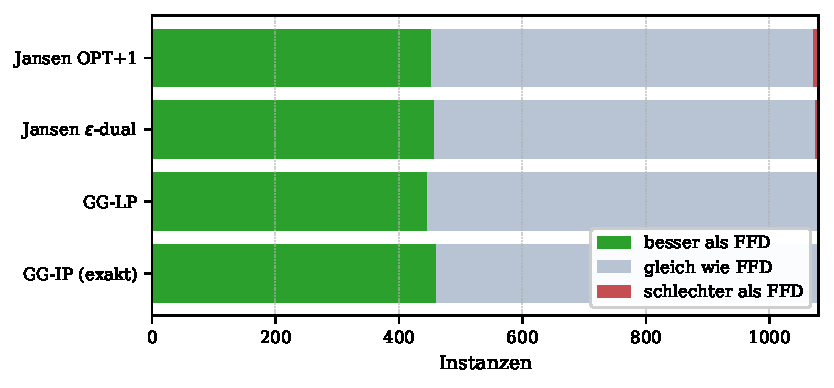
\includegraphics[width=0.96\textwidth]{figures/abb_hm_paare.pdf}
\caption{Jede Subroutine gegen die Grundlinie MULTIFIT+FFD.}
\label{fig:hm-paare}
\end{figure}

\subsection{Die Garantien im Test}
\label{sub:hm-garantien}

Weil GG-IP $\mathrm{OPT}[\Gamma, C]$ bei jeder getesteten Kapazität liefert, lassen sich
die Schranken aus Kapitel~\ref{kap:alternative} unmittelbar nachrechnen.

Für den $\mathrm{OPT}+1$-Algorithmus gilt in allen \HmJansenVergleiche{} verglichenen Aufrufen
$\mathrm{J}[\Gamma,C] - \mathrm{OPT}[\Gamma,C] \in \{0,1\}$, wie es
\textcite{jansen_solisoba2010} garantiert; der Wert 1 tritt in \HmJansenPlusEins{} Fällen auf
(\HmJansenUeberOpt), sonst ist die Packung optimal.

Für das Konfigurations-LP erlaubt Lemma~\ref{lem:gg-rundung} den additiven Term $d-1$, hier also
bis zu \HmDMinusEins.
Gemessen wird er nicht annähernd erreicht: Über \HmGGVergleiche{} Aufrufe ist
$\mathrm{GG}[\Gamma,C] - \mathrm{OPT}[\Gamma,C]$ höchstens \HmGGMaxUeberOpt{} und in
\HmGGPlusEins{} Fällen überhaupt von null verschieden.
Auch der Abstand zur LP-Schranke bleibt klein: In \HmGGOhneVerlust{} der Aufrufe gilt
$\mathrm{GG}[\Gamma,C] = \lceil \mathrm{LP}[\Gamma,C] \rceil$, der größte beobachtete Abstand ist
\HmGGRundungsverlustMax.

Nicht ursächlich dafür ist die Trägerschranke $|F| \le d$ aus Lemma~\ref{lem:gg-ecke}: Sie wird
ausgeschöpft.
Die Zahl der fraktionalen Spalten erreicht im Maximum \HmFMax{} und ist in \HmFGleichD{} der
Aufrufe gleich $d$, im Median beträgt sie \HmFMedian.
Klein bleibt der Verlust vielmehr durch die Rundung selbst.
Variante B aus Abschnitt~\ref{sub:gg-rundung} packt den Restbedarf nicht mit einem Bin je
fraktionaler Spalte, sondern nimmt die kleinere der beiden dort beschriebenen Packungen:
In \HmRestAufrufe{} Aufrufen bleibt überhaupt ein Rest; er kostet im Median
\HmRestBinsMedian{} und höchstens \HmRestBinsMax{} Bins und bleibt in \HmRestUnterFAnteil{} der
Fälle unter $|F|$ - genau der Vorsprung des Abrundens, den Bemerkung~\ref{bem:gg-aufrunden}
begründet.
Die kleinere der beiden Packungen stammt dabei \HmRestQuelleFfd-mal von FFD und
\HmRestQuelleMuster-mal aus der Musterpackung; keine der beiden Varianten ist durchweg die
bessere.

Der $\varepsilon$-duale Algorithmus soll eine Last von höchstens $(1+\varepsilon)C$ zulassen, mit
$\varepsilon = 1/(2d-1)$, hier also zwischen \HmEpsTheorieMin{} und \HmEpsTheorieMax.
Ausgeschöpft wird das nicht: Über \HmEpsAufrufe{} Aufrufe überschreitet nur in \HmEpsPositiv{}
Fällen überhaupt ein Bin die Kapazität $C$, und der größte gemessene Wert ist
$\varepsilon = \HmEpsMax$, entsprechend einer Last von höchstens $\HmLastFaktorMax \cdot C$.

\paragraph{Was MULTIFIT davon merkt.}
Für die Binärsuche zählt nicht die Packung, sondern die Entscheidung über die Kapazität.
Tabelle~\ref{tab:hm-akzeptanz} stellt sie den exakten Werten gegenüber; die letzte Spalte trägt
die Erklärung für den Befund aus Abschnitt~\ref{sub:hm-guete}.
FFD verwirft \HmZuUnrechtFfd{} Kapazitäten, für die eine Packung in $m$ Bins existiert, der
$\mathrm{OPT}+1$-Algorithmus \HmZuUnrechtJansen.
Jede dieser \HmZuUnrechtJansen{} Ablehnungen ist der Fall $\mathrm{J}[\Gamma,C] = m+1$, der nach
Abschnitt~\ref{sub:anwendbarkeit} zweideutig ist und deshalb konservativ als Ablehnung behandelt
wird.
Beide Verfahren verwerfen also zulässige Kapazitäten, nur an verschiedenen Stellen - deshalb
fällt der Vergleich in Tabelle~\ref{tab:hm-paare} in beide Richtungen aus.
Der $\varepsilon$-duale Algorithmus und das ganzzahlige Programm verwerfen dagegen keine
einzige zulässige Kapazität (Spalte \emph{zu Unrecht} in Tabelle~\ref{tab:hm-akzeptanz}:
\HmZuUnrechtJansendual{} und \HmZuUnrechtGgip).

Ihre beiden Zeilen in Tabelle~\ref{tab:hm-akzeptanz} stimmen vollständig überein, und das gilt
nicht nur in der Summe: Auf allen \HmEpsAkzeptanzInstanzen{} Instanzen akzeptieren die beiden
Verfahren genau dieselben Kapazitäten.
Dennoch liefert der $\varepsilon$-duale auf \HmEpsSchlechterRef{} von ihnen einen größeren
Makespan (Tabelle~\ref{tab:hm-paare}).
Die Ursache kann folglich nicht die Entscheidung über die Kapazität sein, sondern nur die
zurückgegebene Packung: Nach Eigenschaft~(ii) von Definition~\ref{def:eps-dual} darf ein Bin die
Kapazität um den Faktor $1+\varepsilon$ überschreiten, und auf diesen \HmEpsSchlechterRef{}
Instanzen geschieht das - bis zum \HmEpsUeberlastMax-fachen der akzeptierten Kapazität.
Für den Makespan zählt demnach nicht allein, welche Kapazitäten eine Subroutine akzeptiert,
sondern bei einem $\varepsilon$-dualen Verfahren auch, wie hoch es die Bins dabei füllt.

\begin{table}[htbp]
\centering
\small
\begin{tabular}{lrrrrr}
\toprule
& & \multicolumn{2}{c}{Entscheidung} & \multicolumn{2}{c}{davon} \\
\cmidrule(lr){3-4}\cmidrule(lr){5-6}
Subroutine & Aufrufe & angen. & abgel. & zertifiziert & zu Unrecht \\
\midrule
FFD & 7\,056 & 5\,219 & 1\,837 & --- & 774 \\
Jansen OPT+1 & 7\,137 & 5\,573 & 1\,564 & --- & 38 \\
Jansen $\varepsilon$-dual & 7\,146 & 5\,595 & 1\,551 & --- & 0 \\
GG-LP & 7\,124 & 5\,544 & 1\,580 & 1\,485 & 95 \\
GG-IP (exakt) & 7\,146 & 5\,595 & 1\,551 & 1\,551 & 0 \\
\bottomrule
\end{tabular}

\caption{Entscheidungen der Subroutinen über alle getesteten Kapazitäten. \emph{Zertifiziert}
  meint eine Ablehnung mit $\lceil \mathrm{LP} \rceil > m$, aus der nach
  Abschnitt~\ref{sub:gg-multifit} $C < C^{*}_{\max}(\Gamma)$ folgt. \emph{Zu Unrecht} zählt die
  Ablehnungen einer Kapazität, für die $\mathrm{OPT}[\Gamma,C] \le m$ gilt, für die es also eine
  gültige Packung in $m$ Bins gibt.}
\label{tab:hm-akzeptanz}
\end{table}

Beim Konfigurations-LP zerfallen die Ablehnungen wie in Abschnitt~\ref{sub:gg-multifit}
beschrieben: \HmGGZertifiziert{} sind zertifiziert, die übrigen \HmGGUnentschieden{}
unentschieden (\HmGGUnentschiedenAnteil{} aller Aufrufe).
Von diesen \HmGGUnentschieden{} unentschiedenen Ablehnungen betreffen \HmZuUnrechtGglp{} eine
tatsächlich zulässige Kapazität; eine zertifizierte Ablehnung kann das nach
Abschnitt~\ref{sub:gg-multifit} nie sein, da aus ihr $C < C^{*}_{\max}(\Gamma)$ folgt.

\paragraph{Nicht-Monotonie.}
Lemma~\ref{lem:nichtmonotonie} lässt zu, dass $\mathrm{J}[\Gamma,\cdot\,]$ beim Übergang zu einer
größeren Kapazität um eins steigt.
Unter den Kapazitäten, die die Binärsuche selbst besucht, zählt die Messung
\HmJansenNichtMonotonSpur{} derartige Paare.
Auf einer zusammenhängenden Kapazitätsreihe der Instanz \HmNichtMonotonInstanz{} tritt der Fall
dagegen auf: $\mathrm{J}[\Gamma, \HmNichtMonotonC] = \HmNichtMonotonJ$, aber
$\mathrm{J}[\Gamma, \HmNichtMonotonCPlus] = \HmNichtMonotonJPlus$.

\subsection{Laufzeit}
\label{sub:hm-laufzeit}

Tabelle~\ref{tab:hm-laufzeit} und Abbildung~\ref{fig:hm-laufzeit} zeigen die Laufzeit über $d$.
FFD bleibt bei \HmZeitMedianffd{}~ms im Median und ist von $d$ unabhängig; die
High-Multiplicity-Verfahren wachsen mit $d$, wie es die Größe der Konfigurationsmenge erwarten
lässt (im Median \HmQMedian{} Spalten, im Maximum \HmQMax).

\begin{table}[htbp]
\centering
\small
\begin{tabular}{lrrrrrr}
\toprule
& & \multicolumn{5}{c}{Median der Laufzeit [ms]} \\
\cmidrule(lr){3-7}
$d$ & Instanzen & FFD & Jansen OPT+1 & Jansen $\varepsilon$-dual & GG-LP & GG-IP (exakt) \\
\midrule
3 & 270 & 0{,}6 & 43{,}4 & 10{,}8 & 5{,}1 & 8{,}4 \\
4 & 271 & 0{,}6 & 91{,}6 & 20{,}2 & 9{,}9 & 15{,}5 \\
5 & 270 & 0{,}6 & 250{,}1 & 56{,}5 & 26{,}9 & 38{,}9 \\
6 & 269 & 0{,}6 & 673{,}3 & 141{,}6 & 70{,}3 & 111{,}1 \\
\midrule
alle $d$ & 1\,080 & 0{,}6 & 125{,}4 & 25{,}7 & 12{,}8 & 19{,}4 \\
\bottomrule
\end{tabular}

\caption{Median der Laufzeit eines vollständigen Laufs von MULTIFIT je Subroutine, gestaffelt
  nach $d$.}
\label{tab:hm-laufzeit}
\end{table}

\begin{figure}[htbp]
\centering
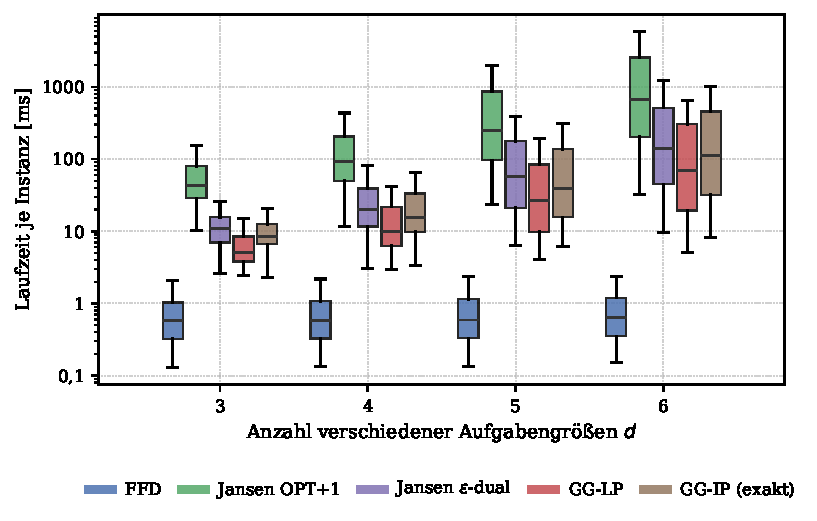
\includegraphics[width=0.94\textwidth]{figures/abb_hm_laufzeit.pdf}
\caption{Laufzeitverteilung je Subroutine über $d$ (logarithmische $y$-Achse, ohne Ausreißer).}
\label{fig:hm-laufzeit}
\end{figure}

Bemerkenswert ist die Reihenfolge: Das \emph{exakte} Konfigurationsprogramm
(\HmZeitMedianggip{}~ms) ist schneller als der $\mathrm{OPT}+1$-Algorithmus
(\HmZeitMedianjansen{}~ms).
Die Ursache ist die Zahl der Aufrufe des Lösers, nicht die Schwere der einzelnen Modelle.
Ein einzelnes MILP des $\mathrm{OPT}+1$-Algorithmus braucht im Median \HmMsProMilpJansen{}~ms und
damit kaum mehr als ein Konfigurationsprogramm mit \HmMsProModellGgip{}~ms.
Die innere Binärsuche nach $m^*$ löst davon je Kapazität jedoch \HmJansenMilpMedian{} Modelle im
Median und bis zu \HmJansenMilpMax, während das Konfigurationsprogramm mit einem auskommt.
Das Maximum ist genau die Schrittzahl einer Binärsuche über $\{1, \ldots, n\}$ bei
$n \le \HmNMax$, nämlich $\lfloor \log_2 \HmNMax \rfloor + 1 = \HmJansenMilpSchranke$.
Die $\varepsilon$-duale Variante, die diese Binärsuche durch die von außen bekannte
Maschinenzahl ersetzt (Abschnitt~\ref{sub:hm-aufbau}), liegt mit \HmZeitMedianjansendual{}~ms
dazwischen.

\subsection{Skalierung in der Multiplizität}
\label{sub:hm-skalierung}

Der Vorteil einer High-Multiplicity-Formulierung liegt darin, dass ihre Größe an der Anzahl $d$
verschiedener Größen hängt und nicht an der Anzahl $n$ der Aufgaben.
Für den $\mathrm{OPT}+1$-Algorithmus ist die Zahl der großen Konfigurationen bei festem $d$
konstant beschränkt (Abschnitt~\ref{sub:jansen-implementierung}).
Auf dem HM-Gitter mit $n \le \HmNMax$ ist das nicht messbar; dafür ist die HM-Skalierung
erzeugt worden.

Das Ergebnis trennt die Verfahren.
Während $n$ um den Faktor \HmSkalNFaktor{} wächst, steigt die Laufzeit von MULTIFIT+FFD um den
Faktor \HmSkalFaktorffd{} (Tabelle~\ref{tab:hm-skalierung}) - FFD verarbeitet jede Aufgabe
einzeln und läuft in $O(n \log n)$ (Abschnitt~\ref{sec:versuchsaufbau}).
Die vier High-Multiplicity-Subroutinen wachsen nur um das \HmSkalFaktorMin- bis
\HmSkalFaktorMax-fache.
Bei $n = \HmSkalNMax$ ist das Konfigurations-LP mit \HmSkalZeitMaxgglp{}~ms um ein Vielfaches
schneller als FFD mit \HmSkalZeitMaxffd{}~ms; der Schnittpunkt der beiden Medianverläufe liegt
nach log-linearer Interpolation zwischen den gemessenen Stützstellen bei etwa
$n \approx \HmSkalSchnittpunkt$ (Abbildung~\ref{fig:hm-skalierung}).

\begin{table}[htbp]
\centering
\small
\begin{tabular}{rrrrrrr}
\toprule
& & \multicolumn{5}{c}{Median der Laufzeit [ms]} \\
\cmidrule(lr){3-7}
$n$ & $m$ & FFD & Jansen OPT+1 & Jansen $\varepsilon$-dual & GG-LP & GG-IP (exakt) \\
\midrule
40 & 5 & 0{,}5 & 105{,}0 & 22{,}6 & 12{,}5 & 18{,}2 \\
400 & 50 & 5{,}7 & 416{,}9 & 55{,}9 & 22{,}7 & 37{,}0 \\
4\,000 & 500 & 79{,}9 & 372{,}7 & 46{,}6 & 23{,}9 & 33{,}8 \\
40\,000 & 5\,000 & 979{,}8 & 991{,}1 & 142{,}2 & 105{,}4 & 124{,}3 \\
\midrule
\multicolumn{2}{l}{Faktor} & 2\,118{,}2 & 9{,}4 & 6{,}3 & 8{,}5 & 6{,}8 \\
\bottomrule
\end{tabular}

\caption{Median der Laufzeit über die Multiplizitätsachse auf dem Datensatz HM-Skalierung,
  bei festem $d \in \{3,4\}$ und festem $n/m$. Die letzte Zeile gibt den Faktor zwischen der
  kleinsten und der größten Instanzgröße an; $n$ selbst wächst dabei um den Faktor
  \HmSkalNFaktor.}
\label{tab:hm-skalierung}
\end{table}

\begin{figure}[htbp]
\centering
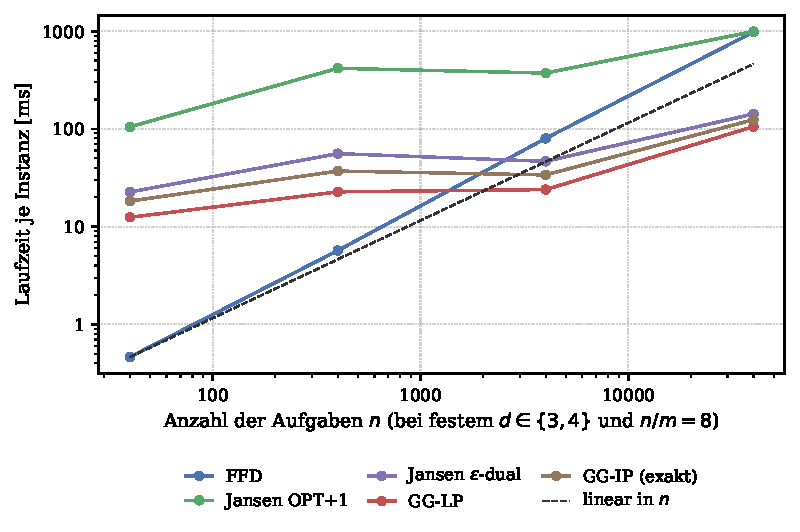
\includegraphics[width=0.92\textwidth]{figures/abb_hm_skalierung.pdf}
\caption{Laufzeit über $n$ bei festem $d \in \{3,4\}$ und festem $n/m$, doppelt logarithmisch.
  Die gestrichelte Linie wächst linear in $n$ und dient als Bezug.}
\label{fig:hm-skalierung}
\end{figure}

\subsection{Einschränkungen dieses Vergleichs}
\label{sub:hm-grenzen}

\begin{itemize}
  \item \textbf{Reichweite in $d$.} Alle Aussagen gelten für $d \le \HmDMax$. Die
    Konfigurationsmenge wächst mit $d$; auf den fünf Datensätzen aus
    Abschnitt~\ref{sec:benchmarks} liegt $d$ im Median zwischen \HmDBenchMedianMin{} und
    \HmDBenchMedianMax{} und damit außerhalb des Bereichs, für den
    Abschnitt~\ref{sub:anwendbarkeit} die Verfahren als sinnvoll ausweist. Gemessen wurden sie
    dort nicht.
  \item \textbf{Der additive Term.} Dass $\mathrm{GG}[\Gamma,C] - \mathrm{OPT}[\Gamma,C]$ hier
    \HmGGMaxUeberOpt{} nicht überschreitet, ist eine Aussage über diese Instanzen und kein Beleg
    gegen die Schranke $d-1$ aus Lemma~\ref{lem:gg-rundung}.
  \item \textbf{Zwei Instanzen mit abweichendem $d$.} In \HmDAbweichung{} Instanzen erzeugt der
    Generator eine Größe mit Vielfachheit null, sodass die Instanz weniger Typen enthält, als ihr
    Name angibt. Die Auswertung liest $d$ deshalb aus dem Instanzinhalt.
  \item \textbf{Laufzeitmessung.} Wie in Abschnitt~\ref{sec:grenzen}: eine Messung je Instanz,
    Mediane über Instanzen statt über Wiederholungen. Die Zeiten gelten für Gurobi in der
    beschriebenen Umgebung; ein anderer Löser verschiebt sie.
\end{itemize}

\chapter{Fazit}
\label{chap:fazit}

Zwei Fragen hat diese Arbeit verfolgt.
Die erste galt der Gütegarantie von MULTIFIT und der Herleitung, welche zu ihr führt.
Die zweite galt der Subroutine, also dem Bin-Packing-Verfahren, das über jede getestete
Kapazität entscheidet.
Beide Stränge treffen sich in Implikation~\eqref{eq:ffd-akzeptiert}: Dort wird aus einer
Eigenschaft der Subroutine eine Aussage über den Makespan.

\paragraph{Die Performanzanalyse.}
Kapitel~\ref{chap:performanz} führt den Nachweis $r_m \le 5/4$ vollständig aus
(Theorem~\ref{thm:schranke54}).
Getragen wird er von Struktureigenschaften eines minimalen Gegenbeispiels: dem Löschlemma, dem
Dominanzlemma, der Mindestzahl von Aufgaben je Bin der $q$-Packung und den Größenschranken.
Theorem~\ref{thm:guete} verbindet das Grenzverhältnis anschließend mit dem Verfahren und liefert
$R_m(\mathrm{MF}(k)) \le r_m + 2^{-k}$.
Die Binärsuche kostet also nur einen additiven Term, welcher sich mit jedem Schritt halbiert.
In die Gegenrichtung führt Lemma~\ref{lem:untere-schranke} den Nachweis $r_m \ge 13/11$ für
$m \ge 13$ an einer Instanz von \textcite{friesen1984}.
Zusammen mit der oberen Schranke von \textcite{cao1995} ist das Grenzverhältnis für diese
Maschinenzahlen exakt bestimmt.

Die Schranke $13/11$ selbst bleibt in dieser Arbeit unbewiesen; Abschnitt~\ref{sec:beweisidee1311} stellt nur
ihre Beweisidee dar.
Caos Fallunterscheidung über $\Delta$ füllt sechzehn Seiten und stützt sich zusätzlich auf
\textcite{yue1990}.
Zwischen der hier bewiesenen Schranke $5/4$ und dem für $m \ge 13$ exakten Wert $13/11$ bleibt
somit eine Lücke; geschlossen wird sie in \cite{cao1995} über diese Fallunterscheidung.

\paragraph{Der Austausch der Subroutine.}
Kapitel~\ref{kap:alternative} prüft drei Alternativen, und die Befunde fallen verschieden aus.
Für MFFD gibt Lemma~\ref{lem:kollaps} eine Klasse von Instanzen an, auf der sich die Wahl
überhaupt nicht auswirkt: Ist die mittlere Maschinenlast mindestens doppelt so groß wie die
größte Aufgabe, in Kurzform $\rho(\Gamma) \ge 2$, so erzeugen MFFD und FFD bei jeder
getesteten Kapazität dieselbe Packung.
Geprüft ist das Kriterium in einem einzigen Durchlauf der Aufgabenliste.
Beim $\mathrm{OPT}+1$-Algorithmus von \textcite{jansen_solisoba2010} entsteht durch die
Modifikation zu einem $\varepsilon$-dualen Verfahren eine eigene Garantie:
Korollar~\ref{kor:multifit-jansen-dual} liefert den Makespan
$(1+\varepsilon)(1+2^{-k}) \cdot C^{*}_{\max}(\Gamma)$ mit $\varepsilon = 1/(2d-1)$, wobei $d$
die Anzahl verschiedener Aufgabengrößen bezeichnet.
Neben der Schranke für MULTIFIT+FFD ist sie die einzige instanzunabhängige Makespan-Garantie
dieser Arbeit; für den $\mathrm{OPT}+1$-Algorithmus selbst gibt Abschnitt~\ref{sub:anwendbarkeit}
eine von der Instanz abhängige Schranke an.

Für das Konfigurations-LP von \textcite{gilmore_gomory1961} fällt das Ergebnis negativ aus.
Lemma~\ref{lem:gg-rundung} lässt nach dem Runden $m + d - 1$ Bins zu und damit gerade die
$d-1$ Bins, die das Akzeptanzkriterium nicht mehr zulässt;
Implikation~\eqref{eq:ffd-akzeptiert} ist folglich nicht erfüllt.
Was das Verfahren stattdessen mitbringt, ist eine zertifizierte Ablehnung: Aus
$\lceil \mathrm{LP}[\Gamma,C] \rceil > m$ folgt $C < C^{*}_{\max}(\Gamma)$, während FFD im
entscheidenden Fall $\mathrm{FFD}[\Gamma,C] = m+1$ nichts über
$\mathrm{OPT}[\Gamma,C]$ aussagt.

\paragraph{Was die Messungen zeigen.}
Auf den \EvalInstanzen{} Instanzen der fünf Benchmark-Datensätze überschreitet kein gemessenes
Verhältnis $13/11$; der größte Wert beträgt \EvalMaxRatioOpt.
MULTIFIT+MFFD liefert dabei in \EvalWins{} Fällen einen kleineren und in \EvalLosses{} Fällen
einen größeren Makespan als MULTIFIT+FFD.
Sämtliche \EvalAbweichungen{} Abweichungen liegen unterhalb von $\rho = 2$, wie es
Lemma~\ref{lem:kollaps} verlangt.
Ein systematischer Vorteil der aufwendigeren Subroutine zeigt sich auf diesen Instanzen nicht.

Die zweite Versuchsreihe trennt Bin-Packing-Güte und Makespan noch deutlicher.
Auf dem HM-Gitter erreicht MULTIFIT+FFD auf \HmOptimalffd{} der Instanzen den optimalen
Makespan, mit dem $\mathrm{OPT}+1$-Algorithmus sind es \HmOptimaljansen.
Gegenüber der Grundlinie gewinnt MULTIFIT mit diesem Algorithmus dennoch nicht durchgängig:
\HmJansenBesserFFD{} Instanzen fallen besser aus, \HmJansenSchlechterFFD{} schlechter.
Den Grund liefert Abschnitt~\ref{sub:hm-garantien}: FFD verwirft \HmZuUnrechtFfd{} Kapazitäten,
für die eine Packung in $m$ Bins existiert, der $\mathrm{OPT}+1$-Algorithmus \HmZuUnrechtJansen{}
- nur an anderen Stellen.
Für den Makespan zählt demnach nicht, wie nah eine Subroutine an $\mathrm{OPT}[\Gamma,C]$
herankommt, sondern welche Kapazitäten sie akzeptiert; genau an diese Entscheidung knüpft
Implikation~\eqref{eq:ffd-akzeptiert} die Gütegarantie von MULTIFIT+FFD.
Die Entscheidung allein trägt den Makespan jedoch nicht: Der $\varepsilon$-duale Algorithmus
akzeptiert nach Abschnitt~\ref{sub:hm-garantien} auf allen \HmEpsAkzeptanzInstanzen{} Instanzen
dieselben Kapazitäten wie das exakte Konfigurationsprogramm und liefert auf
\HmEpsSchlechterRef{} von ihnen dennoch einen größeren Makespan, weil er einen Bin über die
akzeptierte Kapazität hinaus füllen darf.

Die Laufzeiten ordnen sich ebenfalls anders, als es die Güte nahelegt.
Das exakte Konfigurationsprogramm liegt mit \HmZeitMedianggip{}~ms im Median vor dem
$\mathrm{OPT}+1$-Algorithmus mit \HmZeitMedianjansen{}~ms, dessen innere Binärsuche mehrere
Modelle je Kapazität löst.
Wächst die Anzahl der Aufgaben um den Faktor \HmSkalNFaktor, so steigt die Laufzeit von
MULTIFIT+FFD um das \HmSkalFaktorffd-fache, die der High-Multiplicity-Verfahren dagegen nur um
das \HmSkalFaktorMin- bis \HmSkalFaktorMax-fache.

\paragraph{Grenzen der Aussagen.}
Aus den Messungen folgt keine Schranke.
Dass auf \EvalInstanzen{} Instanzen kein Verhältnis über $13/11$ auftritt, ist für
MULTIFIT+FFD mit der bewiesenen Schranke verträglich und begründet für MULTIFIT+MFFD keine.
Ähnliches gilt für das Kollaps-Lemma: Es beschreibt eine Klasse, auf der die Subroutinenwahl
folgenlos bleibt, und gerade der bekannte Extremfall liegt außerhalb, denn die Instanz von
\textcite{friesen1984} hat $\rho = 1{,}65$.
Zur oberen Schranke trägt das Lemma somit nichts bei.

Die zweite Versuchsreihe deckt zudem nur $d \le \HmDMax$ ab, während die fünf
Benchmark-Datensätze im Median zwischen \HmDBenchMedianMin{} und \HmDBenchMedianMax{}
verschiedene Aufgabengrößen enthalten; dort sind die High-Multiplicity-Verfahren nicht gemessen
worden.
Ein Teil der verwendeten Optima stammt aus \textcite{akram2025} und ist nicht nachgerechnet
worden, und sämtliche Laufzeiten gelten für die beschriebene Implementierung und Umgebung.

\paragraph{Offene Fragen.}
Die naheliegendste betrifft MFFD.
Auf der Instanz von \textcite{friesen1984} liefert MULTIFIT+MFFD den kleineren Makespan
(Abschnitt~\ref{sec:friesen}); über das Verhalten im schlechtesten Fall sagt das jedoch nichts,
und ob $r_m(\mathrm{MF}{+}\mathrm{MFFD}) < 13/11$ gilt, bleibt offen.
Dahinter steht die allgemeinere Frage, für welche Subroutinen eine Entsprechung
von~\eqref{eq:ffd-akzeptiert} überhaupt besteht: Für FFD ist sie bewiesen, für MFFD und für das
Konfigurations-LP unbekannt - beim Konfigurations-LP reicht die Rundungsschranke aus
Lemma~\ref{lem:gg-rundung} dafür nicht aus, ein Gegenbeispiel ist damit aber nicht gegeben.
Unbestimmt bleibt ferner das Grenzverhältnis für kleine Maschinenzahlen, denn
Lemma~\ref{lem:untere-schranke} setzt $m \ge 13$ voraus; für $2 \le m < 13$ klafft zwischen
$r_m \ge 1$ aus Bemerkung~\ref{bem:rm-mindestens-eins} und der oberen Schranke $13/11$ eine
Lücke, und nur $r_1 = 1$ ist bestimmt.

Neu entstanden ist die Frage nach der Reichweite der $\varepsilon$-dualen Konstruktion.
Über die von \textcite{jansen_solisoba2010} übernommene Wahl $\varepsilon = 1/(2d-1)$ wird ihre
Garantie mit wachsender Anzahl verschiedener Aufgabengrößen schärfer, die Laufzeit des
Verfahrens nach Abschnitt~\ref{sub:jansen-laufzeit} jedoch doppelt exponentiell in $d$.
Lemma~\ref{lem:jansen-dual} selbst verlangt diese Kopplung nicht; sie begrenzt die Zahl der
großen Konfigurationen und damit die Größe des Programms.
Am schwächsten ist die Garantie demnach dort, wo sie sich berechnen lässt.
Die in Abschnitt~\ref{sub:gg-modell} beschriebene Spaltengenerierung hält das
Konfigurationsmodell auch bei wachsendem $d$ handhabbar; implementiert ist sie hier nicht, und
auf das ganzzahlige Programm des $\varepsilon$-dualen Verfahrens ist sie nicht übertragen
worden.
Zu klären wäre schließlich, ob sich die zertifizierte Ablehnung des Konfigurations-LPs mit einer
schnellen Subroutine verbinden lässt, welche das Suchintervall zwar nicht beweisbar eingrenzt,
dafür aber deutlich schneller entscheidet (Abschnitt~\ref{sub:hm-laufzeit}).


\printbibliography

\cleardoublepage
\thispagestyle{empty}

\section*{Eigenständigkeitserklärung}

Hiermit versichere ich, dass ich die vorliegende Arbeit selbstständig verfasst
und keine anderen als die angegebenen Quellen und Hilfsmittel benutzt habe.

Ich versichere zudem, dass ich diese Arbeit in keinem anderen Prüfungsverfahren
eingereicht habe.

Außerdem versichere ich, dass die beim Prüfungsamt eingereichte gedruckte
Fassung dieser Arbeit mit der eingereichten digitalen Fassung übereinstimmt.

\bigskip

Bei der Anfertigung dieser Arbeit habe ich KI-gestützte Werkzeuge, insbesondere
große Sprachmodelle, als Hilfsmittel eingesetzt. Sie dienten der Literatur- und
Quellenrecherche, der Überprüfung von Zitaten und bibliografischen Angaben, der
sprachlichen Überarbeitung einschließlich Vorschlägen zu Formulierung und
Gliederung sowie dem Auffinden inhaltlicher, formaler und typografischer Fehler.
Darüber hinaus unterstützten sie mich beim Schreiben von \LaTeX{}-Code, bei der
Implementierung der Benchmark-Pipelines in Python sowie bei der Erstellung der
Skripte, welche die Tabellen und Abbildungen aus den Messdaten erzeugen. Die
untersuchten Algorithmen habe ich selbst implementiert.

Die mathematischen Konstruktionen und Beweise sowie die Analysen der empirischen
Tests sind meine eigene Leistung, ebenso die Auswahl und Anordnung der
dargestellten Ergebnisse. Sämtliche Ausgaben
KI-gestützter Werkzeuge habe ich geprüft, bei Bedarf überarbeitet und in eigener
Verantwortung übernommen. Für den Inhalt dieser Arbeit trage ich allein die
Verantwortung.

\vspace{2.5cm}

\noindent
\begin{tabular}{@{}p{5cm}@{\hspace{2cm}}p{7cm}@{}}
    \hrulefill & \hrulefill \\[2pt]
    Ort, Datum & Unterschrift
\end{tabular}


\end{document}
